% !TEX encoding = IsoLatin
\documentclass[spanish,a4paper,12pt]{article}
\usepackage[utf8]{inputenc}
\usepackage[T1]{fontenc}
\usepackage[es-noshorthands]{babel}
\usepackage[dvips]{graphicx}
\usepackage{graphicx}
\usepackage{subcaption}
\usepackage{amsmath,amssymb,amsthm}
\usepackage{mathrsfs}
\usepackage{arydshln}
\usepackage{jgn}
\usepackage{fancyheadings}
\usepackage[thinlines,thiklines]{easybmat}
\usepackage[export]{adjustbox}
\usepackage{babel}
\decimalpoint

\usepackage{pdfpages}

% IMAGEBOX
\def\imagebox#1#2{\vtop to #1{\null\hbox{#2}\vfill}}


\usepackage[top=25mm,left=20mm,body={170mm,255mm}]{geometry}
\usepackage{hyperref}

\usepackage[scaled]{beramono}

\usepackage[framed,numbered,autolinebreaks,useliterate]{mcode}

\usepackage{upquote}
\usepackage{xcolor}
\usepackage{listings}
\usepackage{caption}


\lstset{language=Matlab,breaklines=false,numbers=none}

\lstset{literate=
  {á}{{\'a}}1 {é}{{\'e}}1 {í}{{\'i}}1 {ó}{{\'o}}1 {ú}{{\'u}}1
  {Á}{{\'A}}1 {É}{{\'E}}1 {Í}{{\'I}}1 {Ó}{{\'O}}1 {Ú}{{\'U}}1
  {à}{{\`a}}1 {è}{{\`e}}1 {ì}{{\`i}}1 {ò}{{\`o}}1 {ù}{{\`u}}1
  {À}{{\`A}}1 {È}{{\'E}}1 {Ì}{{\`I}}1 {Ò}{{\`O}}1 {Ù}{{\`U}}1
  {ä}{{\"a}}1 {ë}{{\"e}}1 {ï}{{\"i}}1 {ö}{{\"o}}1 {ü}{{\"u}}1
  {Ä}{{\"A}}1 {Ë}{{\"E}}1 {Ï}{{\"I}}1 {Ö}{{\"O}}1 {Ü}{{\"U}}1
  {â}{{\^a}}1 {ê}{{\^e}}1 {î}{{\^i}}1 {ô}{{\^o}}1 {û}{{\^u}}1
  {Â}{{\^A}}1 {Ê}{{\^E}}1 {Î}{{\^I}}1 {Ô}{{\^O}}1 {Û}{{\^U}}1
  {?}{{\oe}}1 {?}{{\OE}}1 {æ}{{\ae}}1 {Æ}{{\AE}}1 {ß}{{\ss}}1
  {?}{{\H{u}}}1 {?}{{\H{U}}}1 {?}{{\H{o}}}1 {?}{{\H{O}}}1
  {ç}{{\c c}}1 {Ç}{{\c C}}1 {ø}{{\o}}1 {å}{{\r a}}1 {Å}{{\r A}}1
  {?}{{\EUR}}1 {£}{{\pounds}}1
}

 


 \hypersetup{
 colorlinks,
 breaklinks=true,backref,bookmarksnumbered=true,
 pdfauthor={GMC},
 pdftitle={Práctica 3. Tema 1. Modelo de elementos finitos para una fibra elastica 1D}}
% \usepackage{subfigure}


\selectspanish
\title{\vspace*{-4ex}
	\bf\normalsize
	Métodos Computacionales en Ingeniería Civil\\
	\Large
	Práctica \#3, Tema 1.\\
	Modelo de elementos finitos para una barra elástica 1D\\[3ex]
%	\parbox[c]{0.4\textwidth}{%
%%	\includegraphics[width=0.45\linewidth]{sc-nh-post/nh-neoh-0.png}
%%	\includegraphics[width=0.45\linewidth]{sc-nh-post/nh-neoh-1.png}%
%	}%
%	\parbox[c]{0.6\textwidth}{%
	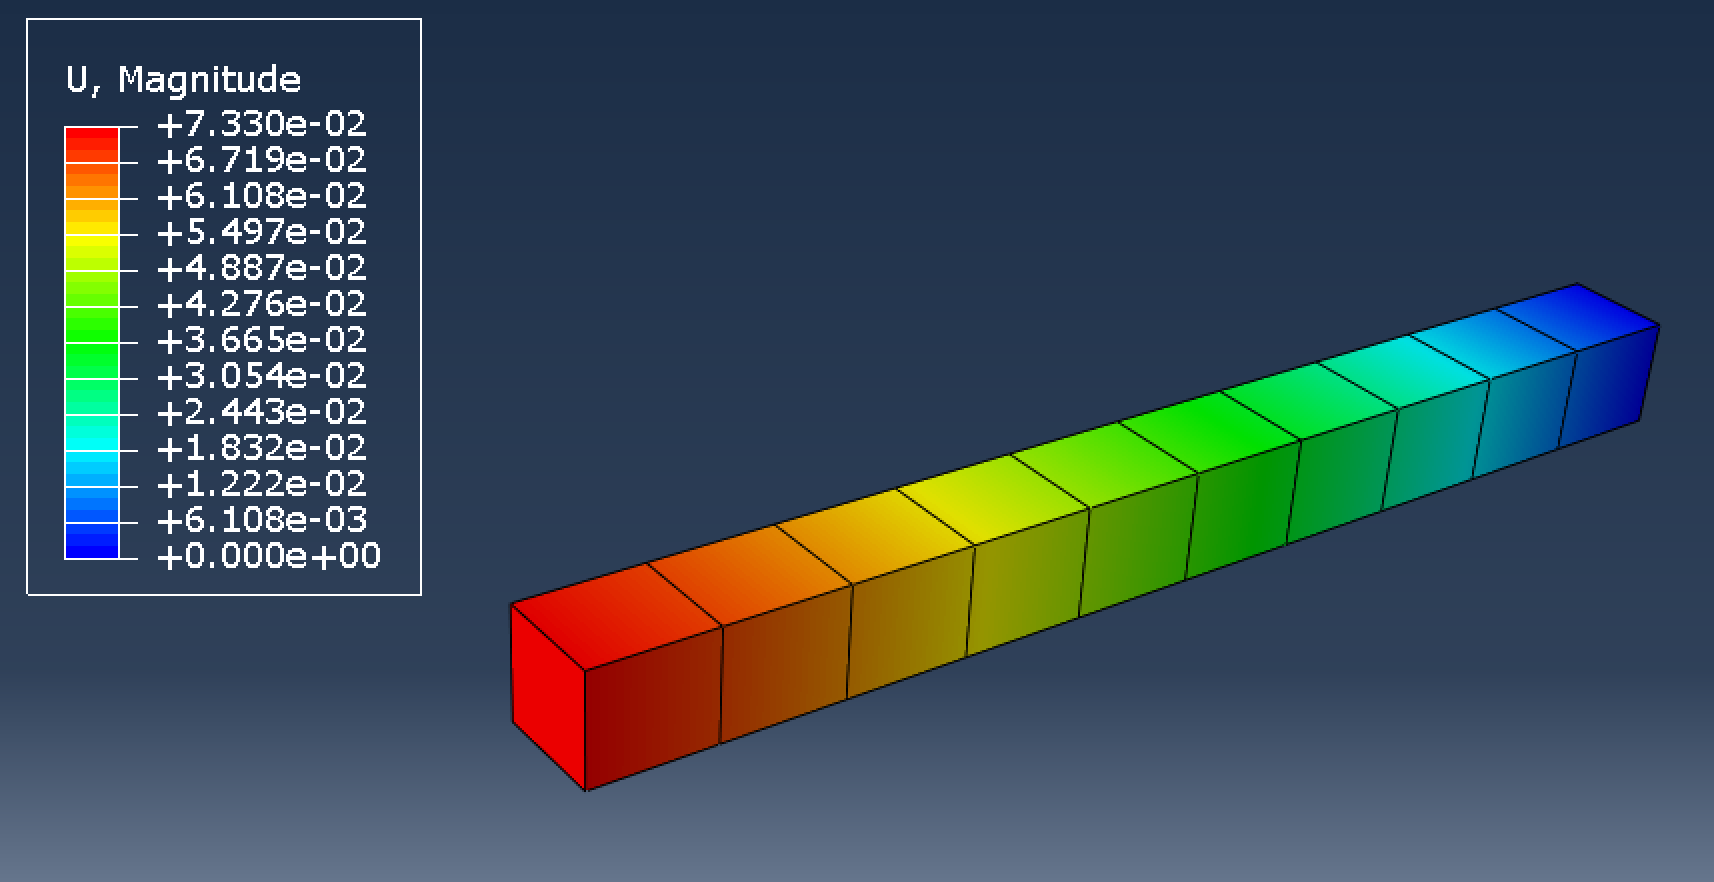
\includegraphics[width=0.65\linewidth]{figuras/barra_portada.png}%
	%}
	}
\author{%José M.ª Goicolea, Pedro Navas, Juan José Arribas, A. Cámara\\
        {\small\sc 
	Grupo de Mecánica Computacional, ETSICCP, UPM}}
\date{15-16 de febrero de 2023}


\begin{document}

\pagestyle{fancy}
\lhead[\fancyplain{}{\thepage}]{\fancyplain{}{\rightmark}}
\rhead[\fancyplain{}{\leftmark}]{\fancyplain{}{\thepage}}
\cfoot[\fancyplain{\thepage}{}]{\fancyplain{\thepage}{}}

\renewcommand{\sectionmark}[1]{\markright{\sf Aptdo.\ \thesection. #1}{}}
\renewcommand*\lstlistingname{Código}

\maketitle

\tableofcontents

\addtocontents{toc}{\protect\hrule}

\clearpage

\section{Objetivos de la práctica}
\label{sec:objetivos}

En esta práctica se ejemplifica la programación en lenguaje \texttt{Python} de un código de elementos finitos, capaz de resolver un problema elástico en una dimensión en el que se somete a cargas una barra estructural en 1D. Se incluye también en el Apéndice este programa para ser ejecutado mediante el software \texttt{Matlab/Octave}. Partimos de las siguientes premisas:
\begin{enumerate}
	\item
	En las bases teóricas tenemos una serie de nociones en cuanto a la construcción de matrices de rigidez elementales, las cuales han de ser programadas por el alumnado.
	\item
	A su vez, estas matrices elementales han de pasar a formar parte de un sistema global a través del ensamblado de la matriz de rigidez global, para la cual también se dispone de ciertas nociones teóricas.
	\item
	Para la resolución del sistema de ecuaciones es necesario conocer las condiciones de contorno de carga y desplazamiento del problema. Se han de aplicar las mismas al sistema matricial que se ha desarrollado en lenguaje \texttt{Python}.
\end{enumerate}

A su vez, vamos a simular una barra similar a la resuelta en \texttt{Python} en 1D con la suite \texttt{Abaqus}. Esto nos ayudará a asimilar los conceptos básicos de dicha suite en 3D, tanto el preproceso, cálculo y postproceso, que nos ayudarán en las siguientes prácticas. De los resultados pretendemos la comparación con una solución analítica.

Los resultados obtenidos por los dos métodos numéricos explicados, \texttt{Python} y  \texttt{Abaqus}, se pueden comparar con solución analítica que el propio alumno ha de obtener. Dicha comparación ha de ser llevada a cabo con las herramientas de dibujo disponibles.


\section{Base teórica y discretización con Elementos Finitos}
\label{sec:teoria}

%\subsection{Governing equations}
\subsection{Ecuaciones de gobierno}

La ecuación que gobierna el fenómeno físico es la de una barra elástica cuyo  desplazamiento se define por \(u(x)\). Como se ha descrito, esta es una ecuación elíptica lineal en una dimensión, con la siguiente forma:
\begin{equation}\label{eq:gov}
\frac{\mathrm{d (A \sigma)}}{\mathrm{d} x} + q(x)
=\frac{\mathrm{d}}{\mathrm{d} x}\left(EA \frac{\mathrm{d} u}{\mathrm{d} x}\right)+q(x)=0
\end{equation}
donde  $E$ es el módulo de Young, un parámetro elástico del material que describe su rigidez. $q(x)$ representa las fuerzas disribuidas para este problema, por unidad de longitud $x$. La resolución numérica de este problema supone encontrar un \(u(x)\), en el intervalo abierto $(0,L)$, tal que el sistema esté en equilibrio teniendo en cuenta unas condiciones de contorno definidas para el problema en cuestión.

\subsection{Condiciones de cortorno y fuerzas volumétricas}

Las posibles condiciones de contorno que nos encontramos en el problema a resolver se resumen en la Fig.~\ref{fig:CC1D}.

\begin{figure}[!htp]
\centering
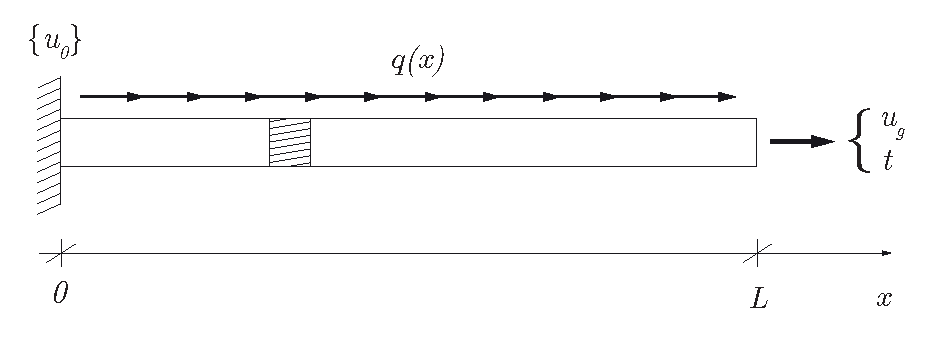
\includegraphics[width=0.8\textwidth]{figuras/1D.pdf}
\caption{Definición del problema y sus condiciones de contorno.}
\label{fig:CC1D}
\end{figure}

Sobre las condiciones de contorno, nos podemos encontrar de dos tipos:
\begin{itemize}
\item \textit{Tipo Dirichlet o Esenciales}\\
Aquellas que se aplican en el campo en el que hemos definido la ecuación diferencial, en nuestro caso \(u(x)\). En este caso son condiciones de contorno ``en desplazamiento''.
$$
u(0)=u_0
$$$$
u(L)=u_g
$$
\item \textit{Tipo Neumann o Naturales}\\
Aquellas que se aplican en la derivada espacial del campo en el que hemos definido la ecuación diferencial, que teniendo en cuenta la ecuación constitutiva, sería:
$$
t= EA \frac{\mathrm{d} u}{\mathrm{d} x} \biggr\rvert_{x=L}
$$
Estas podrían considerarse como condiciones de contorno ``en fuerzas''.
\end{itemize}

Por otro lado nos encontramos las \textit{fuerzas volumétricas o distribuidas}, aquellas que se aplican a todo el dominio y que en la ecuación~\eqref{eq:gov} están definidas por $q(x)$. Estas fuerzas pueden depender de la posición o bien ser constantes.
Un ejemplo de este tipo de fuerzas en el problema mecánico son aquellas asociadas a la gravedad $g$, las cuales dependen de una sección $A(x)$ y una densidad que puede variar a lo largo del dominio, por lo que dicha fuerza también variaría con la posición:
\begin{equation*}
q(x) =A(x) \rho(x) g
\end{equation*}
En el ejemplo a resolver en esta práctica, $q(x)$ será una función dada dependiente de la posición $x$, que representa la carga aplicada por unidad de longitud.

\subsection{Formulación fuerte y solución analítica}
\label{sec:analitica}
La ecuación \eqref{eq:gov} se puede considerar como la formulación fuerte del problema, que se denomina así porque se obliga a que la ecuación en derivadas parciales se cumpla en cada punto del intervalo de interés, $(0,L)$. 

Como vemos, dicha ecuación involucra una derivada segunda del campo \(u(x)\), lo que implica que dicho campo ha de ser derivable dos veces con respecto a $x$.\\

A continuación se detalla la obtención de la solución analítica, para la cual supondremos que el área $A$ y el módulo de Young $E$ son constantes para toda la barra. Partimos de la integración de la formulación fuerte entre un punto $y\in(0,L)$ y L:
\begin{eqnarray}
A \int_y^L \frac{\mathrm{d \sigma}}{\mathrm{d} x} \mathrm{d} x &=& -\int_y^L  q(x) \mathrm{d} x \\
\sigma(L)-\sigma(y) &=& -\frac{1}{A}\int_y^L  q(x) \mathrm{d} x 
\end{eqnarray}
Si empleamos la definición que nos aporta la ecuación constitutiva, $\sigma = E\, \dr u/\dr x$:
\begin{equation}
E \frac{\mathrm{d} u(y)}{\mathrm{d} y} = E \frac{\mathrm{d} u}{\mathrm{d} x} \biggr\rvert_{x=L}  +\frac{1}{A}\int_y^L  q(x) \mathrm{d} x 
\end{equation}
De nuevo, integramos entre 0 y un punto $z\in(0,L)$:
\begin{equation}
\int_0^z E \frac{\mathrm{d} u(y)}{\mathrm{d} y} \mathrm{d} y = \int_0^z \left( E \frac{\mathrm{d} u}{\mathrm{d} x} \biggr\rvert_{x=L}  +\frac{1}{A}\int_y^L  q(x) \mathrm{d} x \right) \mathrm{d} y
\end{equation}
Suponiendo conocida la derivada de $u$ con respecto a $x$ en el punto $x=L$, el resultado obtenido de la integral es:
\begin{equation}
E u(z) - E u(0) = E \frac{\mathrm{d} u}{\mathrm{d} x} \biggr\rvert_{x=L} z + \frac{1}{A}\int_0^z\int_y^L  q(x) \mathrm{d} x \mathrm{d} y
\end{equation}
Por tanto, la solución de $u(z)$ resulta:
\begin{equation}\label{eq:anal}
u(z)  = u(0) +  \frac{\mathrm{d} u}{\mathrm{d} x} \biggr\rvert_{x=L} z  +\frac{1}{EA}\int_0^z\int_y^L  q(x) \mathrm{d} x \mathrm{d} y
\end{equation}

La solución analítica de la ecuación~\eqref{eq:anal} depende de dos constantes para las que son necesarias la aplicación de las dos condiciones de contorno que tenemos, $u(0) $ y $\dr u / \dr x |_{x=L}$, condiciones de contorno esencial y natural respectivamente. Para el caso de no tener una condición de contorno natural en el extremo $x=L$ sino una condición en desplazamientos, el término $\dr u / \dr x |_{x=L}$ se puede calcular imponiendo $z=L$, siendo que $u(L)$ es conocido.

Para el caso particular en que las condiciones de contorno sean: $u(0)=0$ (extremo fijo) y $EA\dr u/\dr x|_{L}=P$ (carga $P$ en $x=L$), y la fuerza distribuida sea una función lineal $q(x)=q_{0}+rx$, la expresión de la solución analítica es:
\begin{equation}
\begin{split}
	u(x) &= \frac{1}{EA}\bigg[ 
	\big(P+q_{0}L+r\frac{L^{2}}{2}\big)x - \big(q_{0}\frac{x^{2}}{2}+r\frac{x^{3}}{6}\big) \bigg]
	\\
	\sigma(x) = E\frac{\dr u}{\dr x}
	&=  \frac{1}{A}\bigg[ 
	P+q_{0}(L-x)+\frac{r}{2}(L^{2}-x^{2}) \bigg]
\end{split}
\label{eq:analitica}
\end{equation}

Teniendo en cuenta las hipótesis realizadas, solo podremos obtener expresiones analíticas para valores sencillos de $E(x)$ y $q(x)$, abandonando la idea cuando estos valores se complican, por lo que hemos de buscar soluciones aproximadas. Una de las técnicas más empleadas es la del método de los elementos finitos, para el que necesitamos la forma débil del problema, que pasamos a describir en la siguiente sección.

\subsection{Formulación débil}
\label{sec:debil}

Esta formulación se consigue con una función de ponderación arbitraria $w(x)$, por la que se multiplica la ecuación de la formulación fuerte y se integra sobre todo el dominio:
\begin{equation}\label{eq:debil}
\int_{0}^{L} w \frac{\mathrm{d}}{\mathrm{d} x}\left(EA \frac{\mathrm{d} u}{\mathrm{d} x}\right) \mathrm{d} x+\int_{0}^{L} w q \mathrm{d} x=0
\end{equation}

Integrando por partes el primer término:
\begin{align}\label{eq:partes}
\frac{\mathrm{d}}{\mathrm{d} x}\left[w \cdot EA \frac{\mathrm{d} u}{\mathrm{d} x}\right] &=\frac{\mathrm{d} w}{\mathrm{d} x} \cdot EA \frac{\mathrm{d} u}{\mathrm{d} x} \quad+w \cdot \frac{\mathrm{d}}{\mathrm{d} x}\left(EA \frac{\mathrm{d} u}{\mathrm{d} x}\right) \nonumber\\
\left[w \cdot EA \frac{\mathrm{d} u}{\mathrm{d} x}\right]_{0}^{L}-\int_{0}^{L} \frac{\mathrm{d} w}{\mathrm{d} x} \cdot EA \frac{\mathrm{d} u}{\mathrm{d} x} \mathrm{d} x &=\int_{0}^{L} w \cdot \frac{\mathrm{d}}{\mathrm{d} x}\left(EA \frac{\mathrm{d} u}{\mathrm{d} x}\right) \mathrm{d} x
\end{align}
obtenemos el resultado siguiente sustituyendo en la ecuación~\eqref{eq:debil}:
\begin{equation}\label{eq:debil1}
\int_{0}^{L} \frac{\mathrm{d} w}{\mathrm{d} x} \cdot EA \frac{\mathrm{d} u}{\mathrm{d} x} \mathrm{d} x=\int_{0}^{L} w q \,\mathrm{d} x+w(L) t_{L}-w(0) t_{0}
\end{equation}
donde $t_{L}$ y $t_{0}$ son las condiciones de contorno naturales en los extremos, que físicamente corresponden a las fuerzas aplicadas en dichos extremos.
Si en el extremo $x=0$ se aplica una condición (esencial) de desplazamiento impuesto o fijo, en este caso a la función de ponderación se le exige también $w(0)=0$, por lo que el último sumando de la ecuación \eqref{eq:debil1} desaparece.

\subsection{Funciones de forma}
\label{sec:N}
En el Método de los elementos finitos es necesario realizar la aproximación de la incógnita $u(x)$ por funciones de aproximación, también llamadas funciones de forma, a través de la expresión:
\begin{equation}\label{eq:N1}
u(x) \approx u_{h}(x)=\sum_{B=1}^{N_{\text {nod }}} u_{B} N_{B}(x)
\end{equation}
Se emplea un conjunto finito $\left(N_{\text {nod }}\right)$ de funciones de interpolación $N_{B}(x)$. Esto conlleva un error que en principio disminuye cuanto mayor sea el número de nodos $N_{\text {nod}}$ o el orden de las funciones de interpolación.

El Método de Galerkin, que es el método más empleado y, por tanto, el que vamos a utilizar, emplea para las funciones de ponderación $w(x)$ la misma interpolación que para la función incógnita $u(x)$:
\begin{equation}\label{eq:N2}
w(x) \approx w_{h}(x)=\sum_{A=1}^{N_{\mathrm{nod}}} w_{A} N_{A}(x)
\end{equation}
La interpolación de las derivadas que aparecen en la forma débil será
\begin{equation}\label{eq:N3}
\frac{\mathrm{d} u_{h}}{\mathrm{d} x}=\sum_{B=1}^{N_{\mathrm{nod}}} u_{B} \frac{\mathrm{d} N_{B}}{\mathrm{d} x} ; \quad \frac{\mathrm{d} w_{h}}{\mathrm{d} x}=\sum_{A=1}^{N_{\mathrm{nod}}} w_{A} \frac{\mathrm{d} N_{A}}{\mathrm{d} x}
\end{equation}
Sustituyendo en las integrales de la forma débil (Eq.~\eqref{eq:debil1}), obtenemos:
\begin{equation}\label{eq:N4}
 \int_{0}^{L}\left(\sum_{A=1}^{N_{\mathrm{nod}}} w_{A} \frac{\mathrm{d} N_{A}}{\mathrm{d} x}\right) EA\left(\sum_{B=1}^{N_{\mathrm{nod}}} u_{B} \frac{\mathrm{d} N_{B}}{\mathrm{d} x}\right) \mathrm{d} x = \sum_{A, B=1}^{N_{\mathrm{nod}}} w_{A}\left[\left.\int_{0}^{L} \frac{\mathrm{d} N_{A}}{\mathrm{d} x} EA \frac{\mathrm{d} N_{B}}{\mathrm{d} x} \mathrm{d} x\right] u_{B}\right. 
\end{equation}
donde 
$$\int_{0}^{L} \frac{\mathrm{d} N_{A}}{\mathrm{d} x} EA \frac{\mathrm{d} N_{B}}{\mathrm{d} x} \mathrm{d} x = K_{AB}$$
es decir,  la denominada matriz de rigidez, $\left[\bm{K} \right]$. Análogamente, para las acciones aplicadas o fuentes se obtienen
los términos del vector de fuerzas:
\begin{equation}\label{eq:N5}
\int_{0}^{L}\left(\sum_{A=1}^{N_{\mathrm{nod}}} w_{A} N_{A}\right) q \,\mathrm{d} x=\sum_{A=1}^{N_{\mathrm{nod}}} w_{A} \underbrace{\left[\int_{0}^{L} N_{A} q \,\mathrm{d} x\right]}_{f_{A}^{\mathrm{vol}}}
\end{equation}
\begin{equation}\label{eq:N6}
\left[w \, EA \,\frac{\mathrm{d} u}{\mathrm{d}x} \right]^L_{0}=w(L) t_{L}-w(0) t_{0}=\sum_{A=1}^{N_{\mathrm{nod}}} w_{A} f_{A}^{\mathrm{ext}}
\end{equation}

De las ecuaciones~\eqref{eq:N4},~\eqref{eq:N5} y~\eqref{eq:N6} resulta el siguiente sistema de ecuaciones algebraicas lineales:
\begin{equation}\label{eq:N7}
\sum_{A, B=1}^{N_{\mathrm{nod}}} w_{A} K_{A B} u_{B}=\sum_{A=1}^{N_{\mathrm{nod}}} w_{A}\left(f_{A}^{\mathrm{vol}}+f_{A}^{\mathrm{ext}}\right)=\sum_{A=1}^{N_{\mathrm{nod}}} w_{A} f_{A}
\end{equation}
donde las fuerzas aplicadas se obtienen como suma de las
volumétricas (interiores distribuidas) y las exteriores en el contorno
$$
f_{A}=f_{A}^{\mathrm{vol}}+f_{A}^{\mathrm{ext}}
$$
Y teniendo en cuenta que $w(x)$ son arbitrarias, $w_{A}$ también lo
serán, por lo que se obtiene la ecuación matricial:
\begin{equation}\label{eq:N8}
\sum_{B=1}^{N_{\text {nod }}} K_{A B} u_{B}=f_{A} \quad \Leftrightarrow \quad \mathbox{[\mathbf{K}]\{\mathbf{u}\}=\{\mathbf{f}\}}
\end{equation}

\subsection{Funciones de forma elementales}
\label{sec:N_e}
En la práctica el cálculo de las integrales y la expresión de las
funciones de interpolación se hacen elemento a elemento. Esto
facilita sobremanera el cálculo que se hace con el mismo
algoritmo en cada uno de los elementos, para luego ensamblar
las matrices globales. 
Las funciones de interpolación tienen soporte compacto, es
decir son cero fuera del subdominio $\Omega^{e}$ correspondiente al
elemento $(e)$ en cuestión.
Se establece una numeración y coordenadas locales en cada
elemento, que tienen su correspondencia con las globales. 

En el caso a resolver 1D podemos suponer funciones de forma lineales de dos nodos como los de la figura~\ref{fig:funciones_forma}. 

\begin{figure}[!htp]
\centering
%\input{figuras/func_forma.latex} 
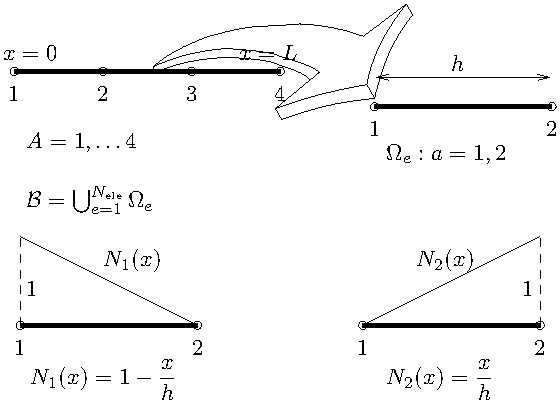
\includegraphics[width=0.6\textwidth]{figuras/func_forma1.pdf}
\caption{Esquema de las funciones de forma lineales del elemento 2 de una discretización 1D de una barra con 3 elementos}
\label{fig:funciones_forma}
\end{figure}

Teniendo en cuenta los valores de $N_1$ y $N_2$ que aparecen en la figura~\ref{fig:funciones_forma}, se realizan las integrales de cada uno de los términos; por ejemplo $K_{11}^{e}$ es:
\begin{equation}\label{eq:N9}
K_{11}^{e}=\int_{0}^{h} \frac{\mathrm{d} N_{1}}{\mathrm{d} x} EA \frac{\mathrm{d} N_{1}}{\mathrm{d} x} \mathrm{d} x=\frac{EA}{h^{2}} h=\frac{EA}{h}
\end{equation}
y análogamente los demás:
\begin{equation}\label{eq:N10}
K_{22}^{e}=\frac{EA}{h} ; \quad K_{12}^{EA}=K_{21}^{e}=-\frac{EA}{h}
\end{equation}
resultando
\begin{equation}\label{eq:N11}
\left[\mathbf{K}^{e}\right]=\frac{EA}{h}\left(\begin{array}{cc}{1} & {-1} \\ {-1} & {1}\end{array}\right)
\end{equation}
Similarmente el vector de fuerzas volumétricas del elemento resulta
\begin{equation}\label{eq:N12}
\left\{\mathbf{f}^{\mathrm{vol}, e}\right\}=\frac{h}{6}\left\{\begin{array}{l}{2q_1+q_2} \\ {q_1 + 2q_2}\end{array}\right\}
\end{equation}

%Si considerásemos una carga repartida constante, dicho vector de fuerzas elemental se podría expresar como:
%\begin{equation}
%\left\{\mathbf{f}^{\mathrm{int}, e}\right\}=q h\left\{\begin{array}{l}{1 / 2} \\ {1 / 2}\end{array}\right\}
%\end{equation}\label{eq:N12_bis}

Una vez formadas las matrices elementales se convierten a
numeración global,
\begin{eqnarray}
K_{a b}^{e} & \rightarrow\left[\hat{\mathbf{K}}^{e}\right] \nonumber
 \\
f_{a}^{e} & \rightarrow \lbrace\hat{\mathbf{f}}^{e}\rbrace \nonumber
\end{eqnarray}
ensamblándose finalmente estas matrices locales dentro de las matrices globales del sistema. Para el ejemplo de la figura~\ref{fig:funciones_forma}, puesto que todos los elementos son iguales, las matrices elementales de rigidez son todas iguales entre sí, siendo su valor el de la matriz de la ecuación~\eqref{eq:N11}.

Para poder realizar el ensamblaje hay que tener en cuenta el lugar que van a ocupar en la matriz de rigidez global las distintas componentes de las matrices de rigidez locales. Si observamos la figura~\ref{fig:funciones_forma} vemos que el elemento 1 y el elemento 2 comparten el nodo número 2, por eso la posición $(2,2)$ de la matriz de rigidez global será compartida por las matrices de rigidez locales de los elementos 1 y 2. La forma que tendrá esta matriz de rigidez global será:

\begin{equation}
  K^{global} = \left[
  \begin{BMAT}[8pt]{cccc}{cccc}
   K_{11}^{(1)} & K_{12}^{(1)} & 0 & 0\\
   K_{21}^{(1)} & K_{22}^{(1)}  + K_{11}^{(2)} & K_{12}^{(2)} & 0 \\
    0 & K_{21}^{(2)} & K_{22}^{(2)} + K_{11}^{(3)}  & K_{12}^{(3)} \\
    0 & 0 & K_{21}^{(3)} & K_{22}^{(3)}
  \addpath{(0,4,.)rrddlluu}
  \addpath{(1,3,.)rrddlluu}
   \addpath{(2,2,.)rrddlluu}
  \end{BMAT}\right]
\end{equation}

De este ensamblaje, teniendo en cuenta los valores de las matrices de rigidez locales, obtenemos la matriz de rigidez global:
$$
[\mathbf{K}]=\frac{EA}{h}\left(\begin{array}{cccc}{1} & {-1} & {0} & {0} \\ {-1} & {1+1} & {-1} & {0} \\ {0} & {-1} & {1+1} & {-1} \\ {0} & {0} & {-1} & {1}\end{array}\right)
$$
Las matrices elementales y global de fuerzas volumétricas son
$$\left\{\mathbf{f}^{\mathrm{vol}, e}\right\}=\frac{h}{6}\left\{\begin{array}{l}{2q_1+q_2} \\ {q_1 + 2q_2}\end{array}\right\}
\Rightarrow\left\{\mathrm{f}^{\mathrm{vol}}\right\}=\frac{h}{6}\left\{\begin{array}{c}{2q_1^{(1)}+q_2^{(1)}} \\ {q_1^{(1)} + 2q_2^{(1)} + 2q_1^{(2)}+q_2^{(2)}} \\ {q_1^{(2)} + 2q_2^{(2)} + 2q_1^{(3)}+q_2^{(3)}}  \\ {q_1^{(3)} + 2q_2^{(3)}}\end{array}\right\}
$$

Si considerasemos una restricción del movimiento en el extremo $x=0$ y una carga $q_L$ aplicada en el extremo $x=L$, la ecuación matricial que resulta de aplicar el método de los Elementos Finitos es:
$$
[\mathbf{K}]\{\mathbf{u}\}=\left\{\mathbf{f}^{\text {vol }}\right\}+\left\{\mathbf{f}^{\text {ext }}\right\}
$$
\begin{equation}\label{sistema}
\frac{EA}{h}\left(\begin{array}{c;{2pt/2pt}ccc}{1} & {-1} & {0} & {0} \\ 
\hdashline[2pt/2pt]
{-1} & {1+1} & {-1} & {0} \\ {0} & {-1} & {1+1} & {-1} \\ {0} & {0} & {-1} & {1}\end{array}\right)
\left\{\begin{array}{l}0\\
\hdashline[2pt/2pt]
u_2 \\ u_{3} \\ u_{4}\end{array}
\right\}=
\frac{h}{6}\left\{\begin{array}{c}{2q_1^{(1)}+q_2^{(1)}} \\ 
\hdashline[2pt/2pt]
{q_1^{(1)} + 2q_2^{(1)} + 2q_1^{(2)}+q_2^{(2)}} \\ {q_1^{(2)} + 2q_2^{(2)} + 2q_1^{(3)}+q_2^{(3)}}  \\ {q_1^{(3)} + 2q_2^{(3)}}\end{array}\right\}
+\left\{\begin{array}{c} R_0 \\
\hdashline[2pt/2pt]
{0} \\ {0} \\ {P}\end{array}\right\}
\end{equation}

\clearpage
 
 Al vector de fuerzas volumétricas se le suma el de externas, en este caso una posible carga en P. Por otro lado, en el extremo $x=0$ existe una reacción para que el desplazamiento sea igual al impuesto, $u(0)=0$. Dicha reacción se calcula \textit{a posteriori,} una vez calculados los desplazamientos $\{\mathbf{u}\}$. \\
 
Una vez calculados los desplazamientos por la inversión de la matriz de rigidez, ya reducida por la aplicación de las condiciones de contorno, cabe la posibilidad de verificar el equilibrio, que se puede obtener como resultado de la suma de las fuerzas internas del cuerpo, que, en el caso del equilibrio, deben ser 0, siendo estas fuerzas internas calculadas como:
 $$
\left\{\mathbf{f}^{\text {int}}\right\}=[\mathbf{K}]\{\mathbf{u}\}
$$
 
 Por otro lado, la reacciñon en este caso se podría calcular multiplicando la fila eliminada de la matriz $[\mathbf{K}]$ por el vector de desplazamientos y restándole las fuerzas aplicadas en dicho nodo, que, al tratarse de un contorno tipo Dirichlet, solo podrán ser fuerzas volumétricas:
 $$
 R_0=K_{1j}u_j-f^{\text {vol}}_1
$$

\paragraph{Observación importante.---}
El hecho de que los valores en los puntos discretos, tanto en tensiones como en desplazamientos, vayan a salir exactamente iguales que los de la solución analítica, es un caso que se denomina \emph{``superconvergente''}. 
Sin embargo, en general las soluciones numéricas en los puntos discretos no coincidirán con la solución exacta.
Dicho de otra manera, en este caso extremadamente sencillo el único error cometido por la solución de elementos finitos es para los valores intermedios en el interior de los elementos, siendo exactos los valores en los nodos y en los puntos de integración; sin embargo, en un caso general, habrá un error numérico también para los valores en los nodos y en los puntos de integración.


\clearpage

\section{Simulación con Abaqus}
\label{sec:abaqus}

Se desea calcular la respuesta de una barra elástica unidimensional, de longitud \(L=10 \mathrm{mm}\)
y sección uniforme \(A=1 \mathrm{mm}^{2} .\) El material es elástico lineal, con módulo de Young \(E=1000 \mathrm{MPa}\).
El extremo izquierdo \((x=0)\) está fijo mientras que sobre el derecho \((x=L)\) actúa una fuerza
axial de valor \(P=5 \mathrm{N},\) como se indica en la figura~\ref{fig:esq}. Se podrá suponer que las deformaciones son pequeñas.

\begin{figure}[!htp]
\centering
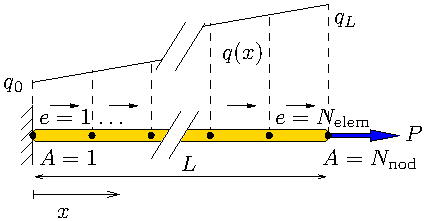
\includegraphics[width=0.7\textwidth]{figuras/esquema.pdf}
\caption{Modelo de fibra elástica 1D}
\label{fig:esq}
\end{figure}

A partir de los dígitos de las centenas (c), decenas (d) y unidades ( \(u\) ) del número de matricula de cada estudiante, \(N_{\text {mat }}=m c d u,\) se tomarán los siguientes parámetros para el modelo:
\begin{itemize}
\item Número de elementos \(N_{\text {elem }}=11-c\)
\item La carga distribuida \(q(x),\) fuerza longitudinal por unidad de longitud, será lineal entre los extremos \(x=0\) y \(x=L,\) con los valores en los extremos \(q_0=d / 10\; \mathrm{N} / \mathrm{mm}, \quad q_{L}=q_{0}+u / 10 \; \mathrm{N} / \mathrm{mm} \).
\end{itemize}

Los pasos que se deberían seguir en una programación del mismo serían:
\begin{enumerate}
\item Planteamiento del problema elástico y condiciones de contorno.
\item Expresiones numéricas de las matrices de rigidez y de fuerzas del modelo completo.
\item Aplicación de condiciones de contorno y resolución.
\item Solución para los desplazamientos \(u(x)\) y tensiones \(\sigma(x)\) en cada punto, dibujando la gráfica en función de \(x\) y comparando con la solución analítica. (Nota: las tensiones se calculan
a partir de los desplazamientos como \(\sigma=E \varepsilon=E \mathrm{d} u / \mathrm{d} x,\) y empleando la aproximación
en un elemento finito, \(\left.\sigma^{h}=E u_{a} \mathrm{d} N_{a} / \mathrm{d} x=E\left(u_{2}-u_{1}\right) / h .\right)\)
\end{enumerate}

En un primer momento vamos a emplear el programa \texttt{Abaqus} para obtener el resultado de dicha barra empleando un software comercial de \emph{elementos finitos}.
Aunque el modelo es unidimensional, decidimos emplear elementos 3D para ayudar a visualizar la geometría de la barra e introducir este tipo de modelado.
Seguiremos los pasos similares a la práctica 1, solo que en este caso vamos a realizar nuestro primer modelo 3D.

\subsection{Módulo \texttt{Part}}

En primer lugar, se ejecuta \emph{Abaqus CAE} para crear un modelo nuevo. Se entra en el módulo \texttt{part}, activando el icono de crear una nueva parte, que se define como 3D, deformable, solid por extrusión (figura \ref{fig:bar1a}). Una vez definido el problema, creamos un rectángulo (figura \ref{fig:bar1b}) en las esquinas (-0.5,-0.5) y (0.5,0.5), por lo que tendremos un area de 1 mm$^2$.
\begin{figure}[h!tp]
\centering
\captionsetup[subfigure]{justification=centering,singlelinecheck=false}
  \begin{subfigure}[b]{0.38\textwidth}
  \hspace{10mm}
    \imagebox{90mm}{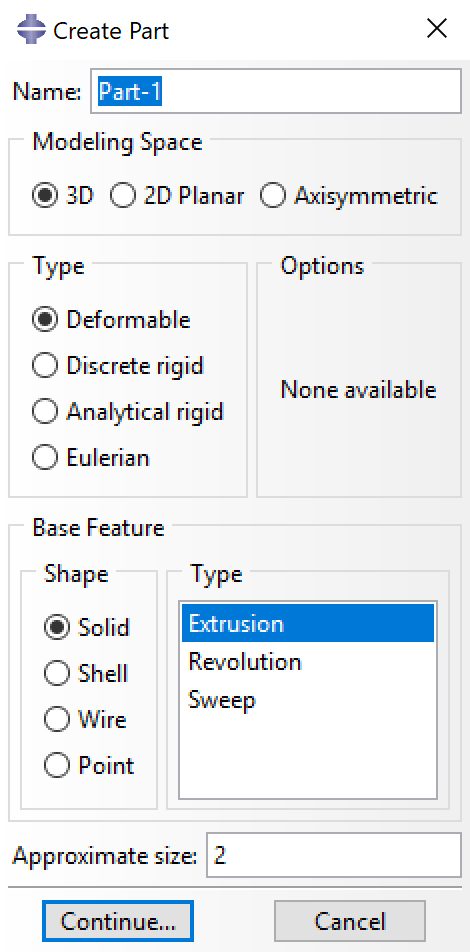
\includegraphics[scale=0.51]{capturas/solid.png}}
    \caption{Part/solid\label{fig:bar1a}}
  \end{subfigure}
  \begin{subfigure}[b]{0.25\textwidth}
  \hspace{6mm}
    \imagebox{90mm}{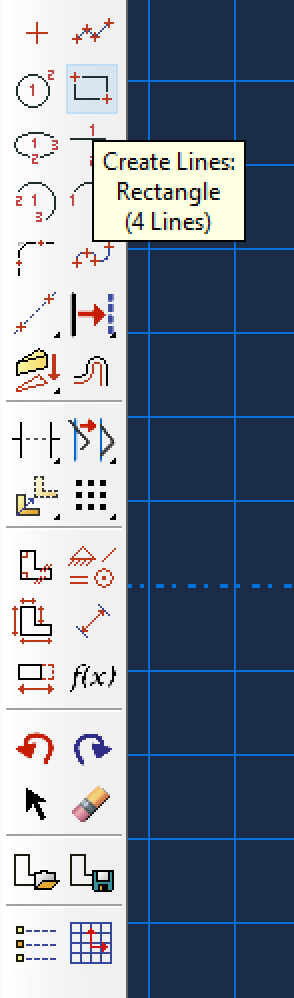
\includegraphics[scale=0.5]{capturas/rectangulo.png}}
    \caption{Rectángulo\label{fig:bar1b}}
  \end{subfigure}
\caption{Creación de geometría}
\label{fig:bar1}
\end{figure}

Una vez definido, hacemos clic en \emph{done} y pasamos a definir la longitud de la barra en la dirección \emph{Z}, que en nuestro caso es 10 mm. Deberíamos obtener un cuerpo similar al del la figura \ref{fig:bar2b}.

\begin{figure}[h!tp]
\centering
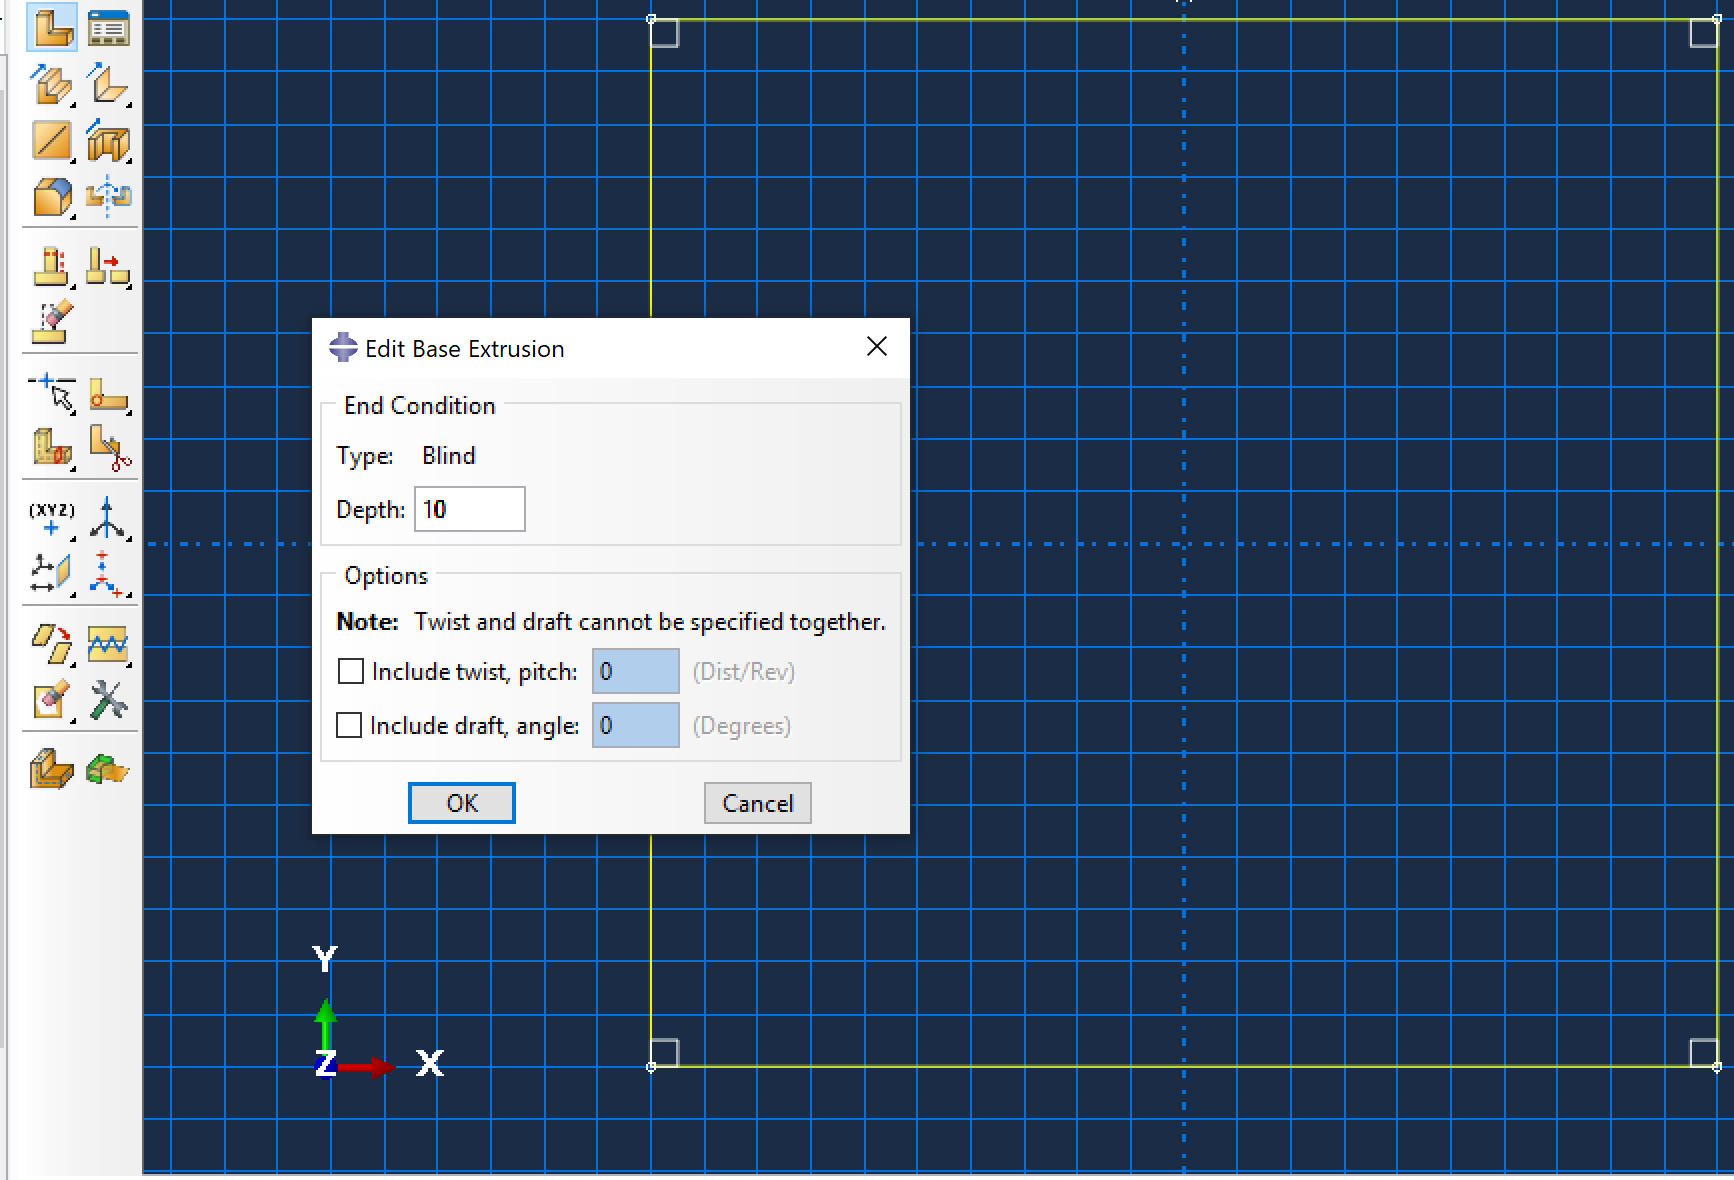
\includegraphics[scale=0.4]{capturas/sec1.png}
\caption{Extrusión de la sección.}
\label{fig:bar2a}
\end{figure}
\begin{figure}[h!tp]
\centering
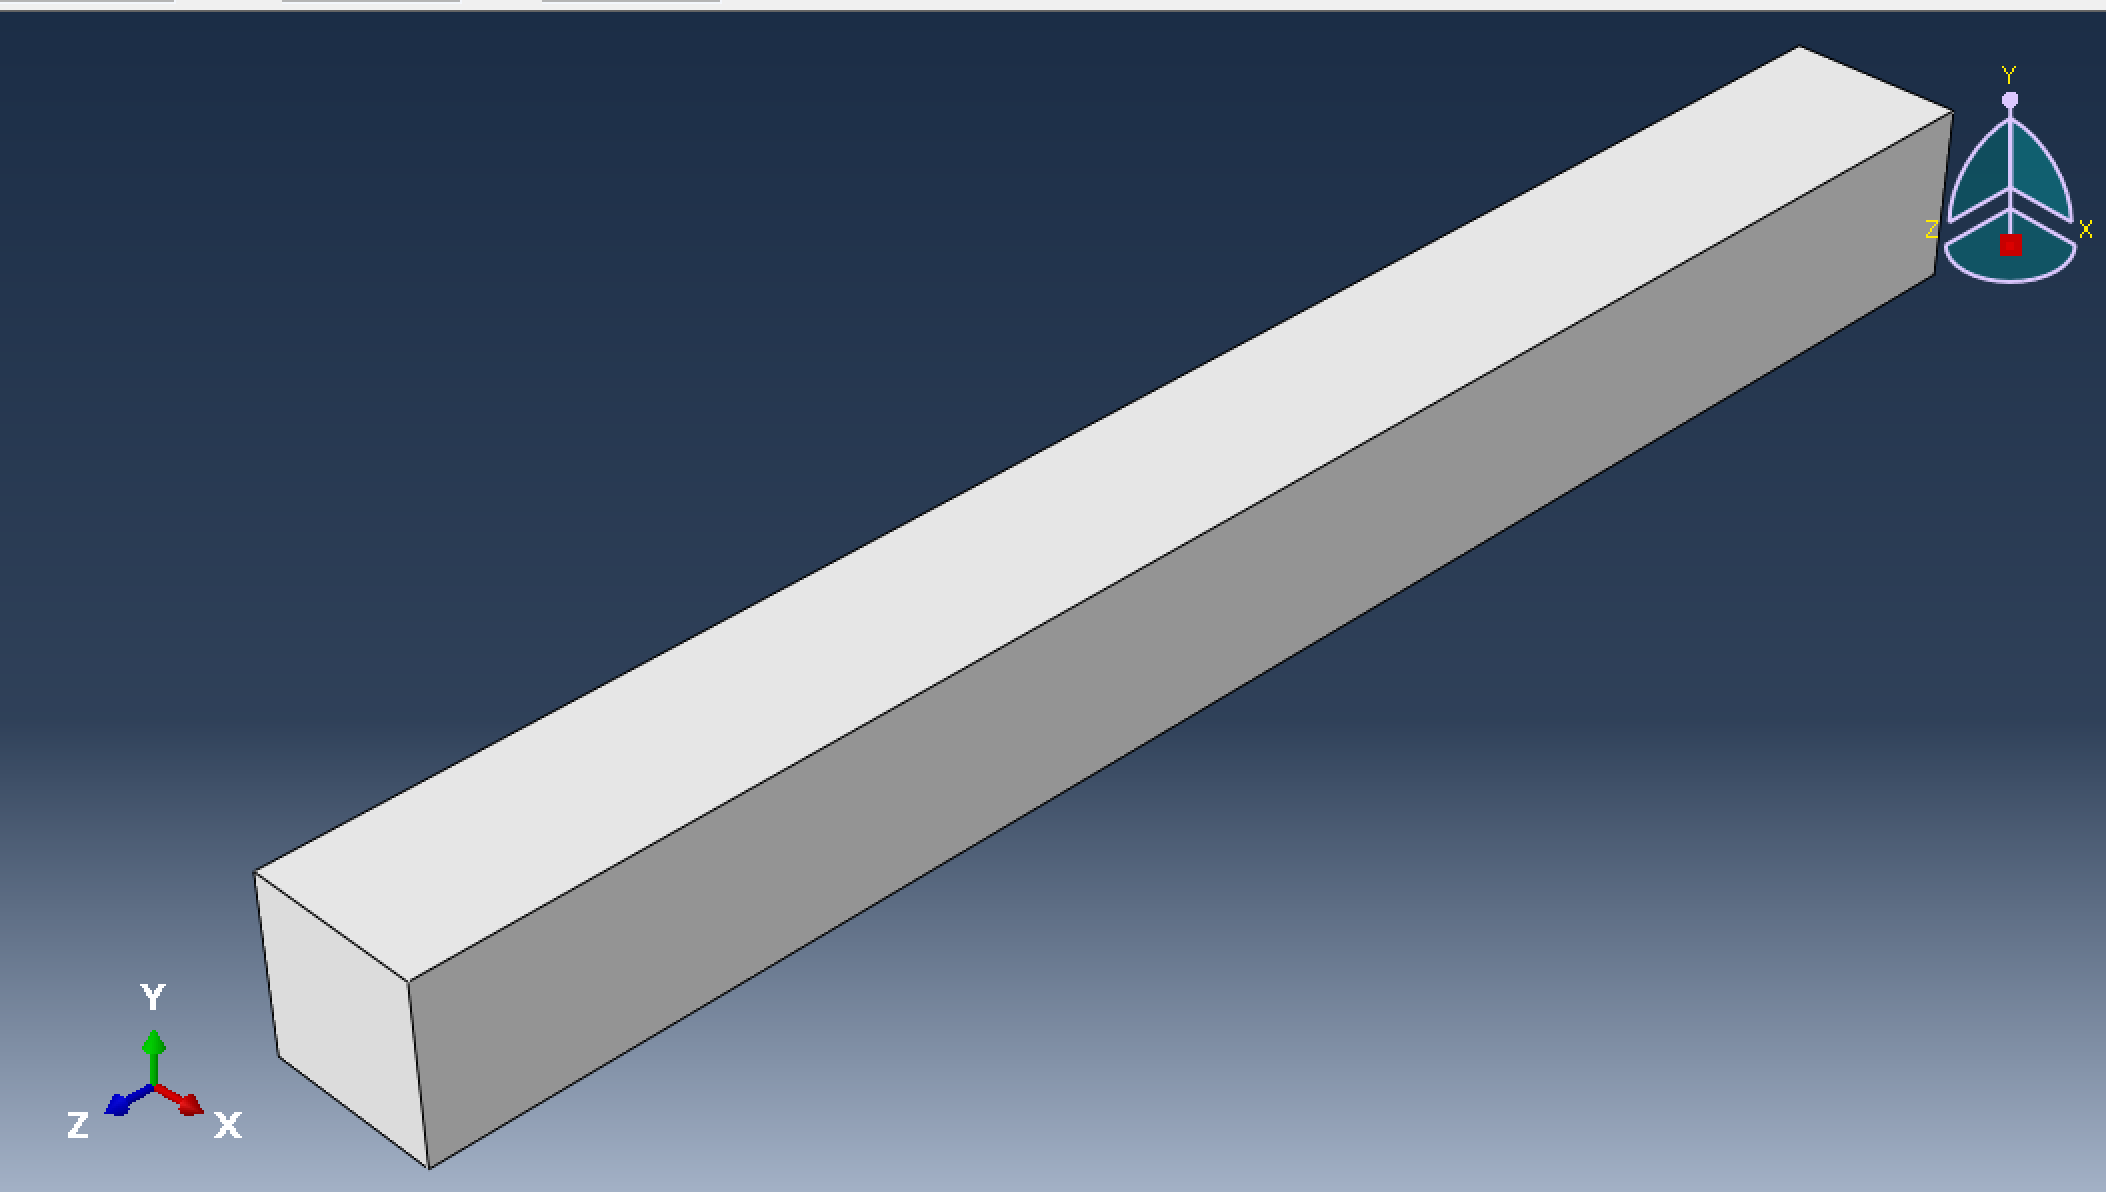
\includegraphics[scale=0.30]{capturas/sec2.png}
\caption{Barra final}
\label{fig:bar2b}
\end{figure}


\subsection{Módulo \texttt{Property}}

Se activa el icono para crear material nuevo,(figura \ref{fig:bar3}),
se selecciona el material elástico lineal y se introducen las propiedades $E=1000\,\text{MPa}, \nu=0$. Hemos de tener en cuenta que al trabajar en mm y N para la carga, debemos introducir el módulo elástico en MPa=N/mm$^2$.  A continuación se crea una \emph{``sección''}, en la que se definen sus propiedades, en este caso solo el tipo de material descrito anteriormente, tipo \emph{solid}-homogéneo (figura \ref{fig:bar4a}).
A continuación se asigna la sección a la parte creada (figura \ref{fig:bar4b}), seleccionando todo el volumen y haciendo clic en \emph{Done}.
\begin{figure}[h!tp]
\centering
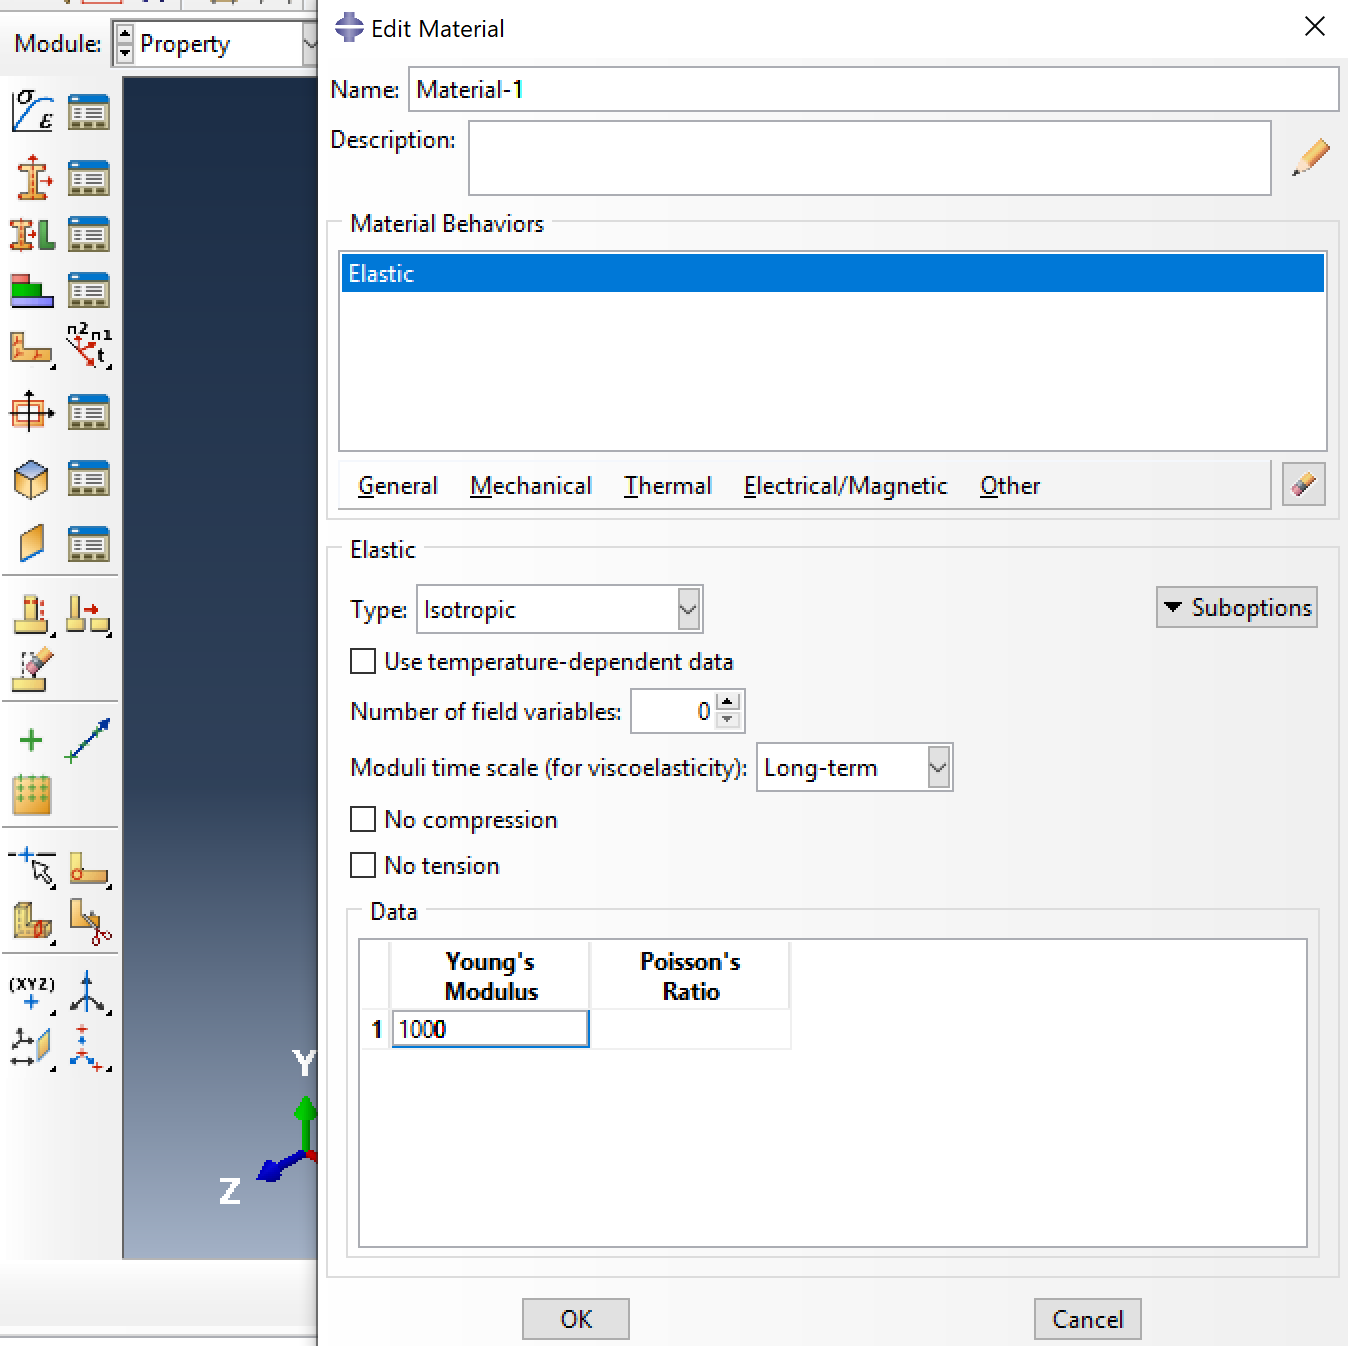
\includegraphics[scale=0.4]{capturas/prop0.png}
\caption{Material elástico.}
\label{fig:bar3}
\end{figure}

\begin{figure}[h!tp]
\centering
\captionsetup[subfigure]{justification=centering,singlelinecheck=false}
  \begin{subfigure}[b]{0.20\textwidth}
  \hspace{0mm}
    \imagebox{75mm}{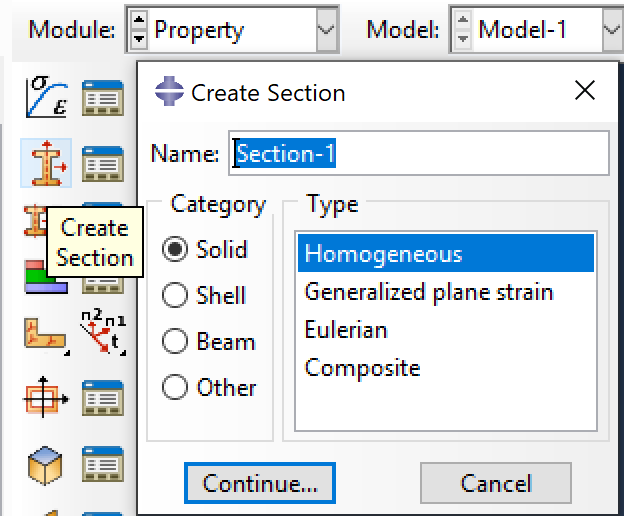
\includegraphics[scale=0.3]{capturas/prop1.png}}
    \caption{Crear sección\label{fig:bar4a}}
  \end{subfigure}
  \begin{subfigure}[b]{0.79\textwidth}
  \hspace{0mm}
    \imagebox{75mm}{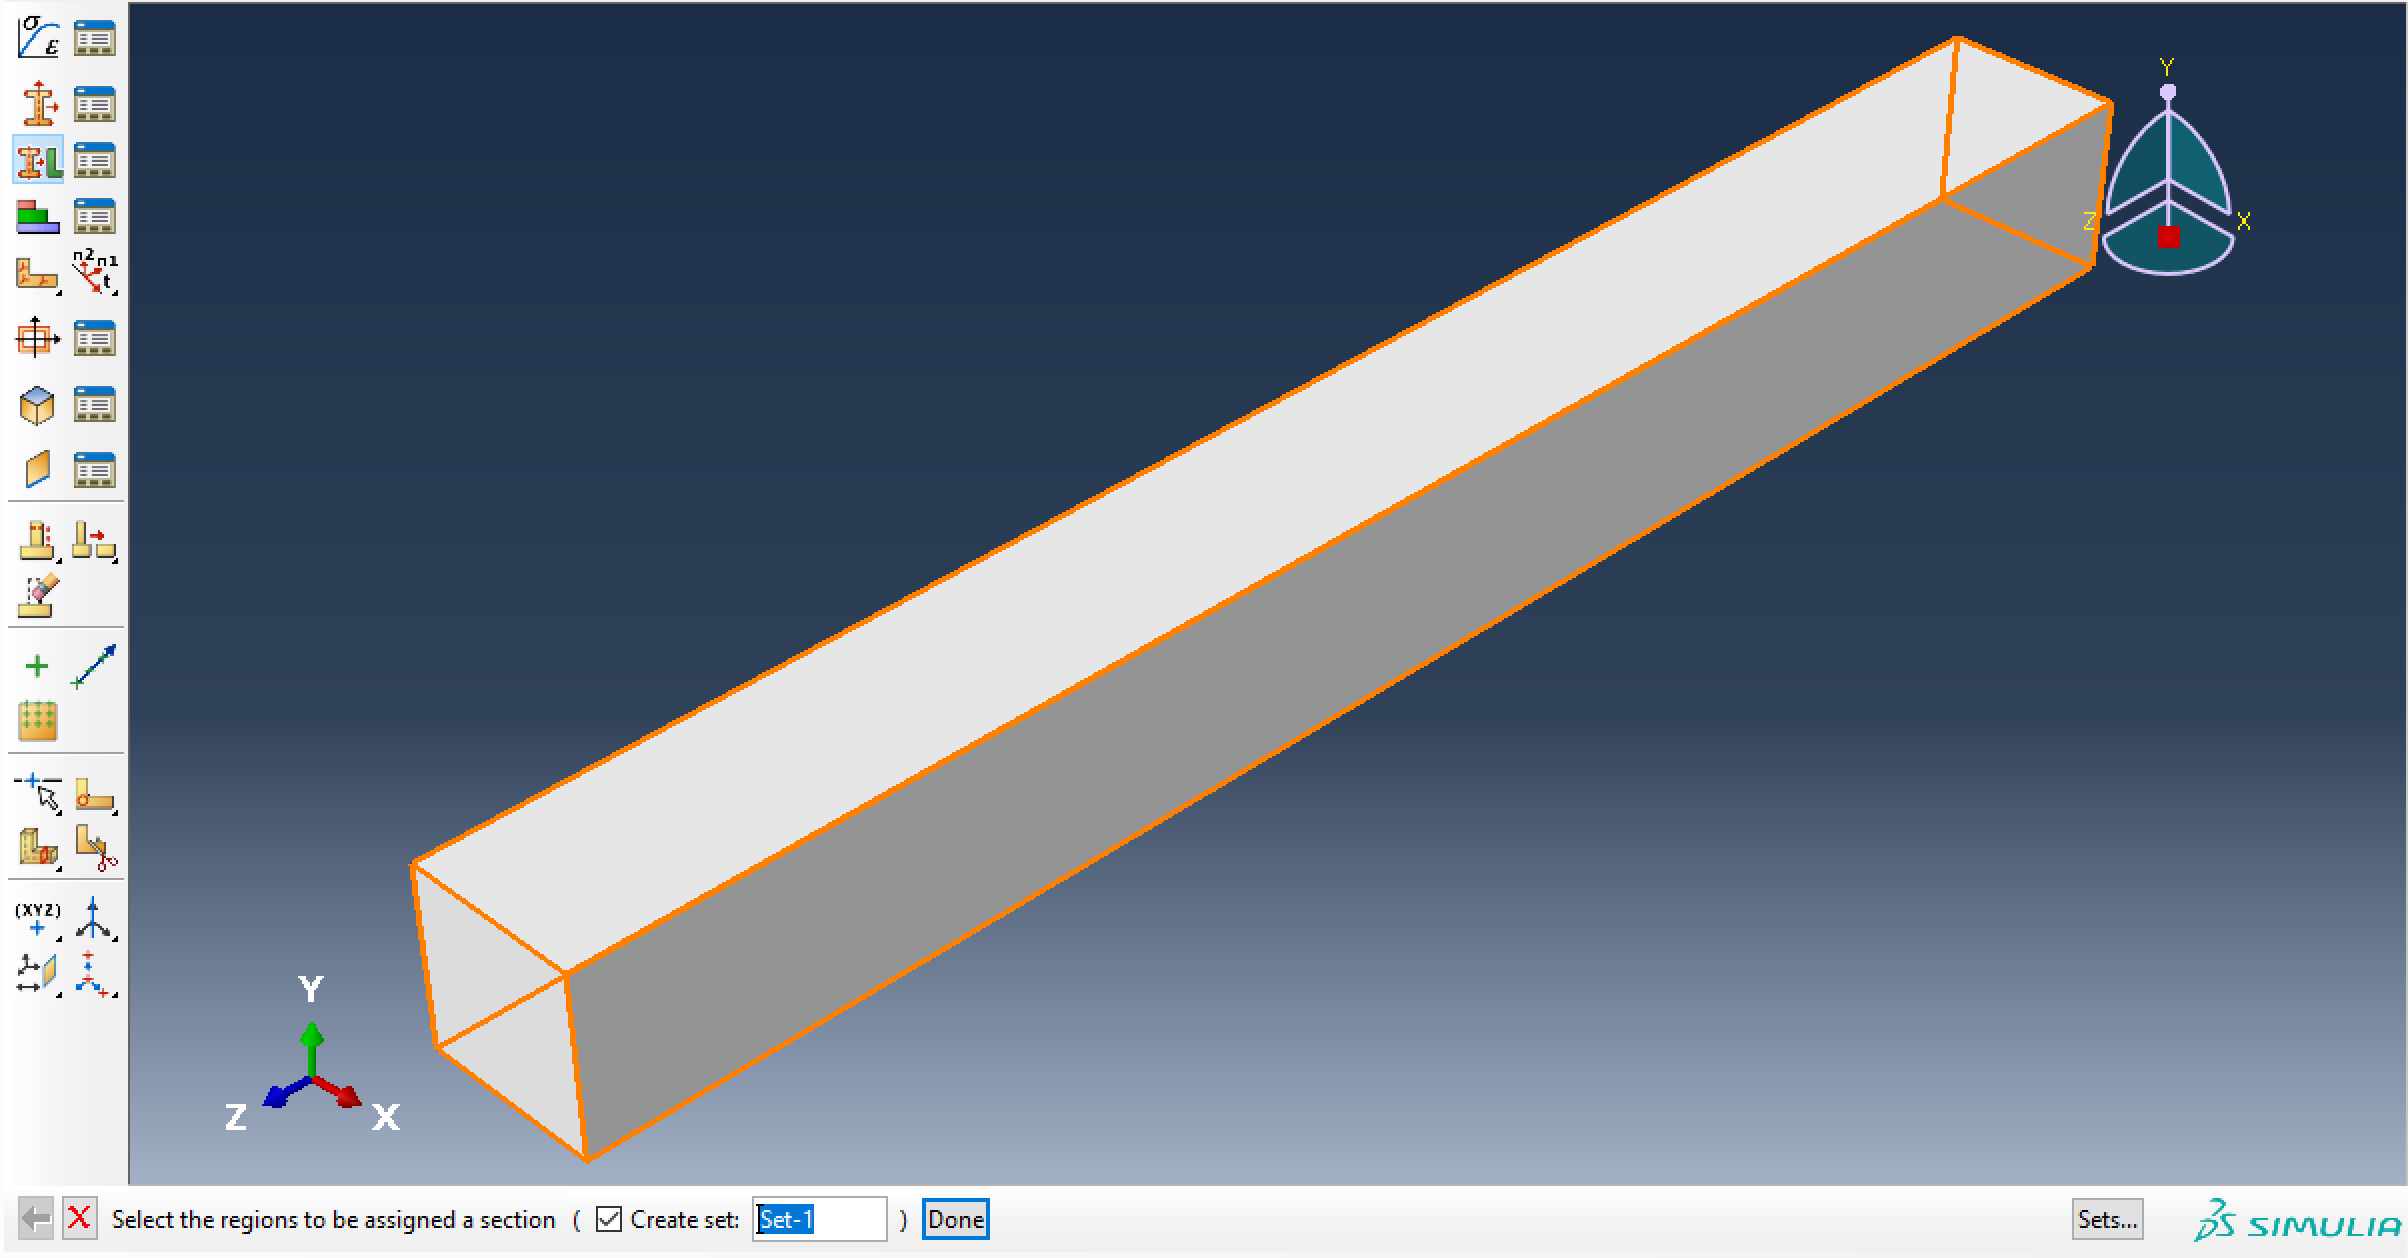
\includegraphics[scale=0.32]{capturas/prop2.png}}
    \caption{Asignar sección\label{fig:bar4b}}
  \end{subfigure}
\caption{Selección de la sección}
\label{fig:bar4}
\end{figure}

\clearpage
\subsection{Módulo \texttt{Assembly}}

En este módulo tan solo hay que crear una ``instancia'' a partir de la parte, mediante las opciones por defecto:
\begin{figure}[h!tp]
\centering
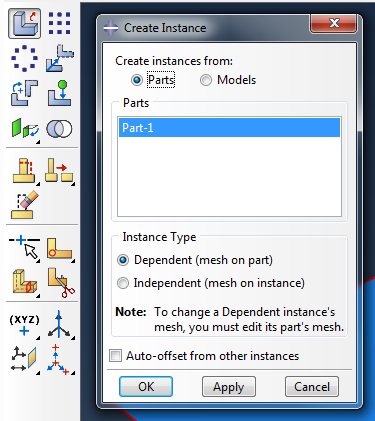
\includegraphics[scale=0.4]{capturas/14-assembly.png}
\caption{Assembly: crea una instancia de la parte}
\label{fig:assembly}
\end{figure}

\subsection{Módulo \texttt{Step}}

Se crea un ``step'' para el procedimiento de cálculo ``Static, general''. Se toman las opciones por defecto (figura \ref{fig:step}). 
No es necesario editar el ``field output'', pues el conjunto de variables de salida por defecto incluye ya las que necesitaremos en nuestro análisis.

\begin{figure}[h!tp]
\centering
\captionsetup[subfigure]{justification=centering,singlelinecheck=false}
  \begin{subfigure}[b]{0.35\textwidth}
  \hspace{10mm}
    \imagebox{90mm}{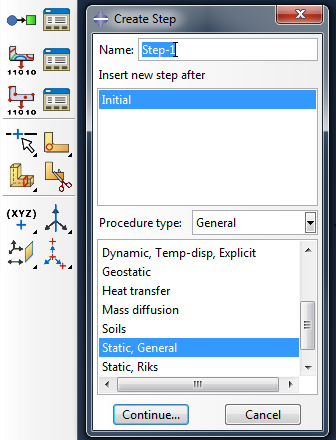
\includegraphics[scale=0.4]{capturas/15-step.png}}
  \end{subfigure}
  \begin{subfigure}[b]{0.64\textwidth}
  \hspace{6mm}
    \imagebox{90mm}{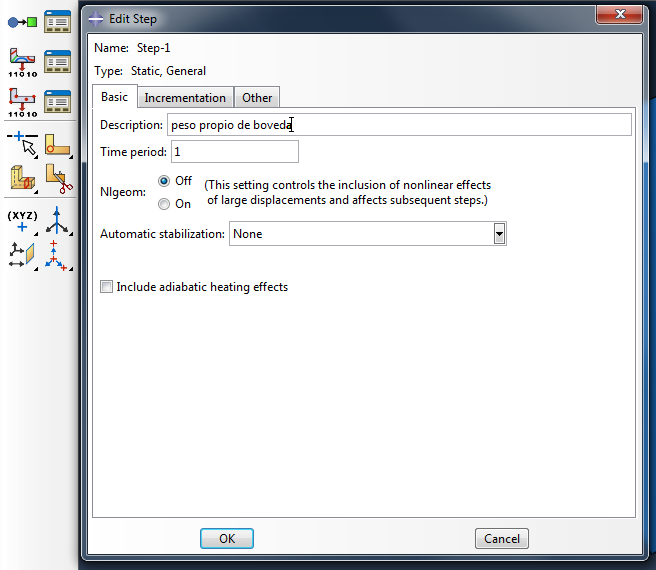
\includegraphics[scale=0.4]{capturas/16-step.png}}
  \end{subfigure}
\caption{Crear y definir el ``step''}
\label{fig:step}
\end{figure}

\clearpage
\subsection{Módulo \texttt{Load}}
Debemos definir en este módulo ambos tipos de condiciones de contorno. En primer lugar, en \emph{Z=0}, empotramos la barra. Para ello creamos \emph{Boundary Condition}, de categoría \emph{Mechanical} y tipo \emph{Encastre} (figura \ref{fig:load1}).

\begin{figure}[h!tp]
\centering
\captionsetup[subfigure]{justification=centering,singlelinecheck=false}
  \begin{subfigure}[b]{0.4\textwidth}
  \hspace{0mm}
    \imagebox{60mm}{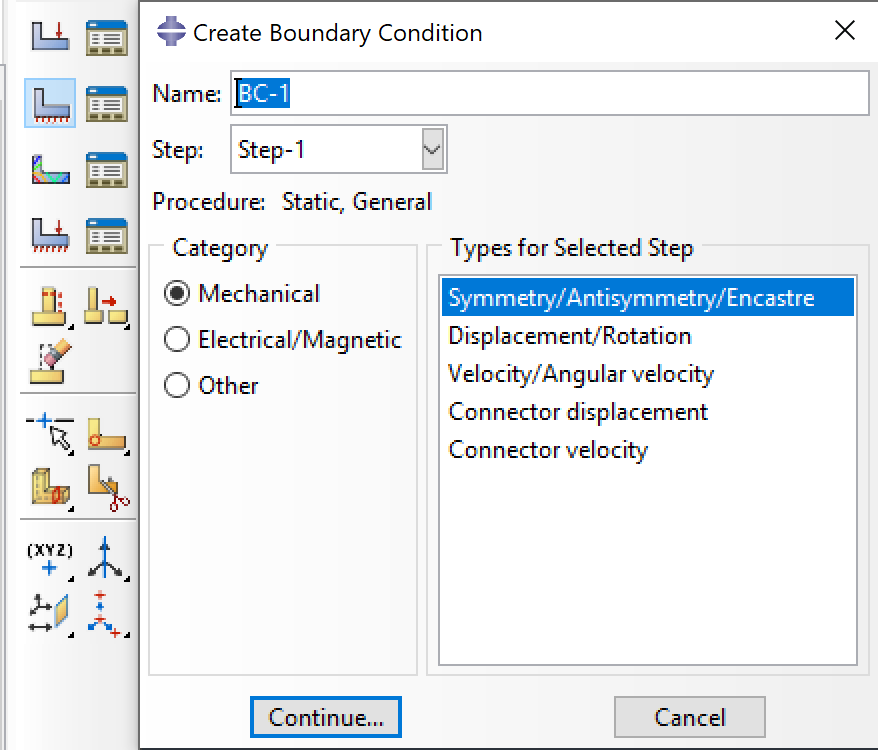
\includegraphics[scale=0.4]{capturas/load1.png}}
  \end{subfigure}
  \begin{subfigure}[b]{0.59\textwidth}
  \hspace{1mm}
    \imagebox{60mm}{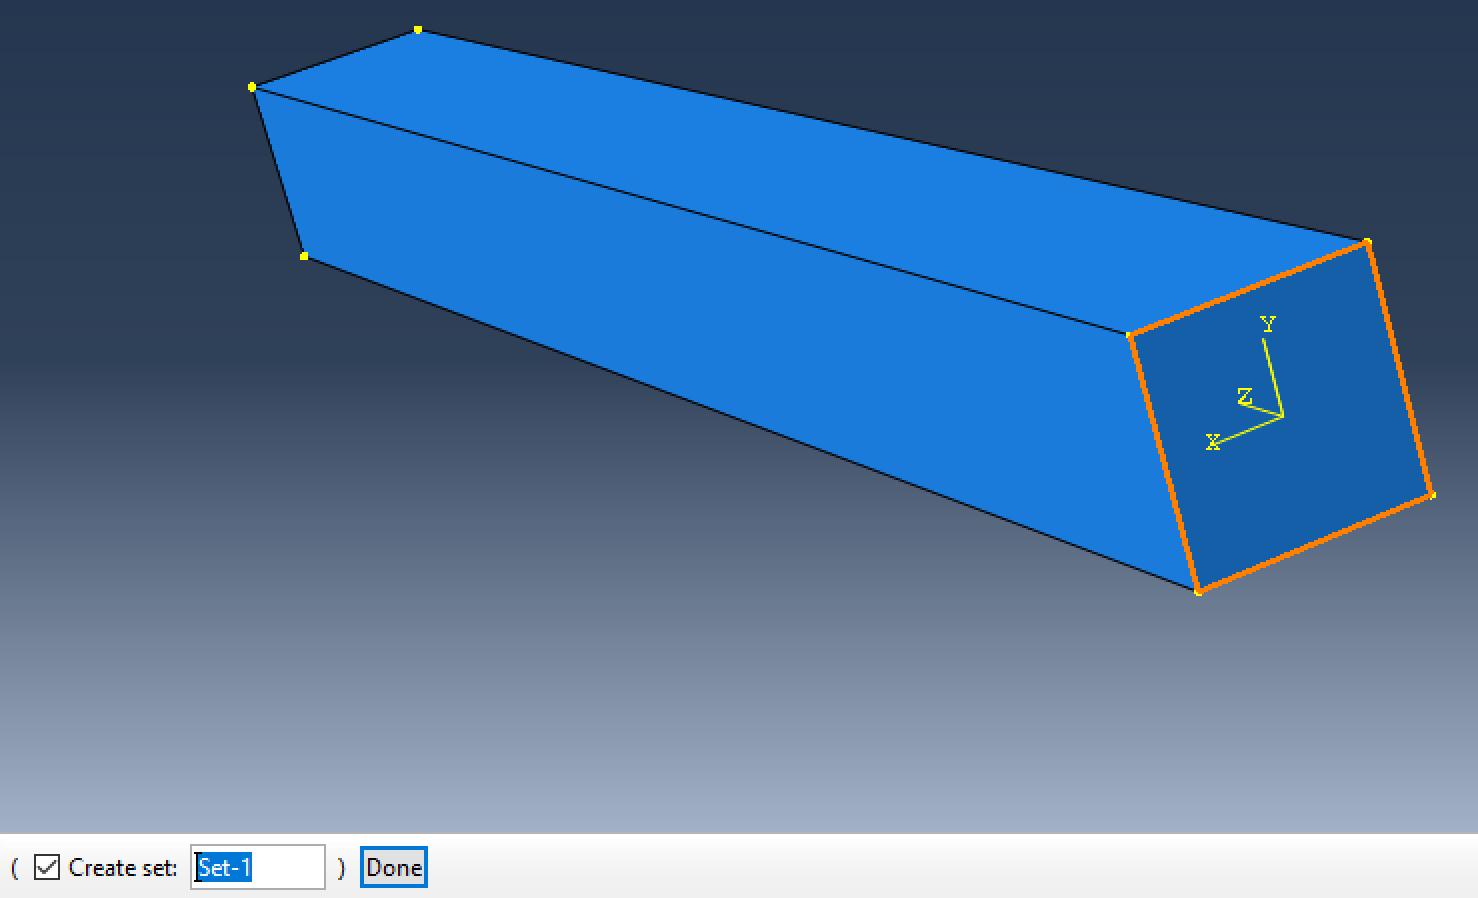
\includegraphics[scale=0.35]{capturas/load2.png}}
  \end{subfigure}
\caption{Creación del empotramiento}
\label{fig:load1}
\end{figure}

Una vez seleccionada la superficie a empotrar y habiendo hecho clic en \emph{Done}, debemos especificar el tipo de condición a asignar dentro de este subgrupo, por lo que seleccionaremos la última de esta nueva pestaña (figura \ref{fig:load2}), donde menciona la opción \emph{Encastre}.

\begin{figure}[h!tp]
\centering
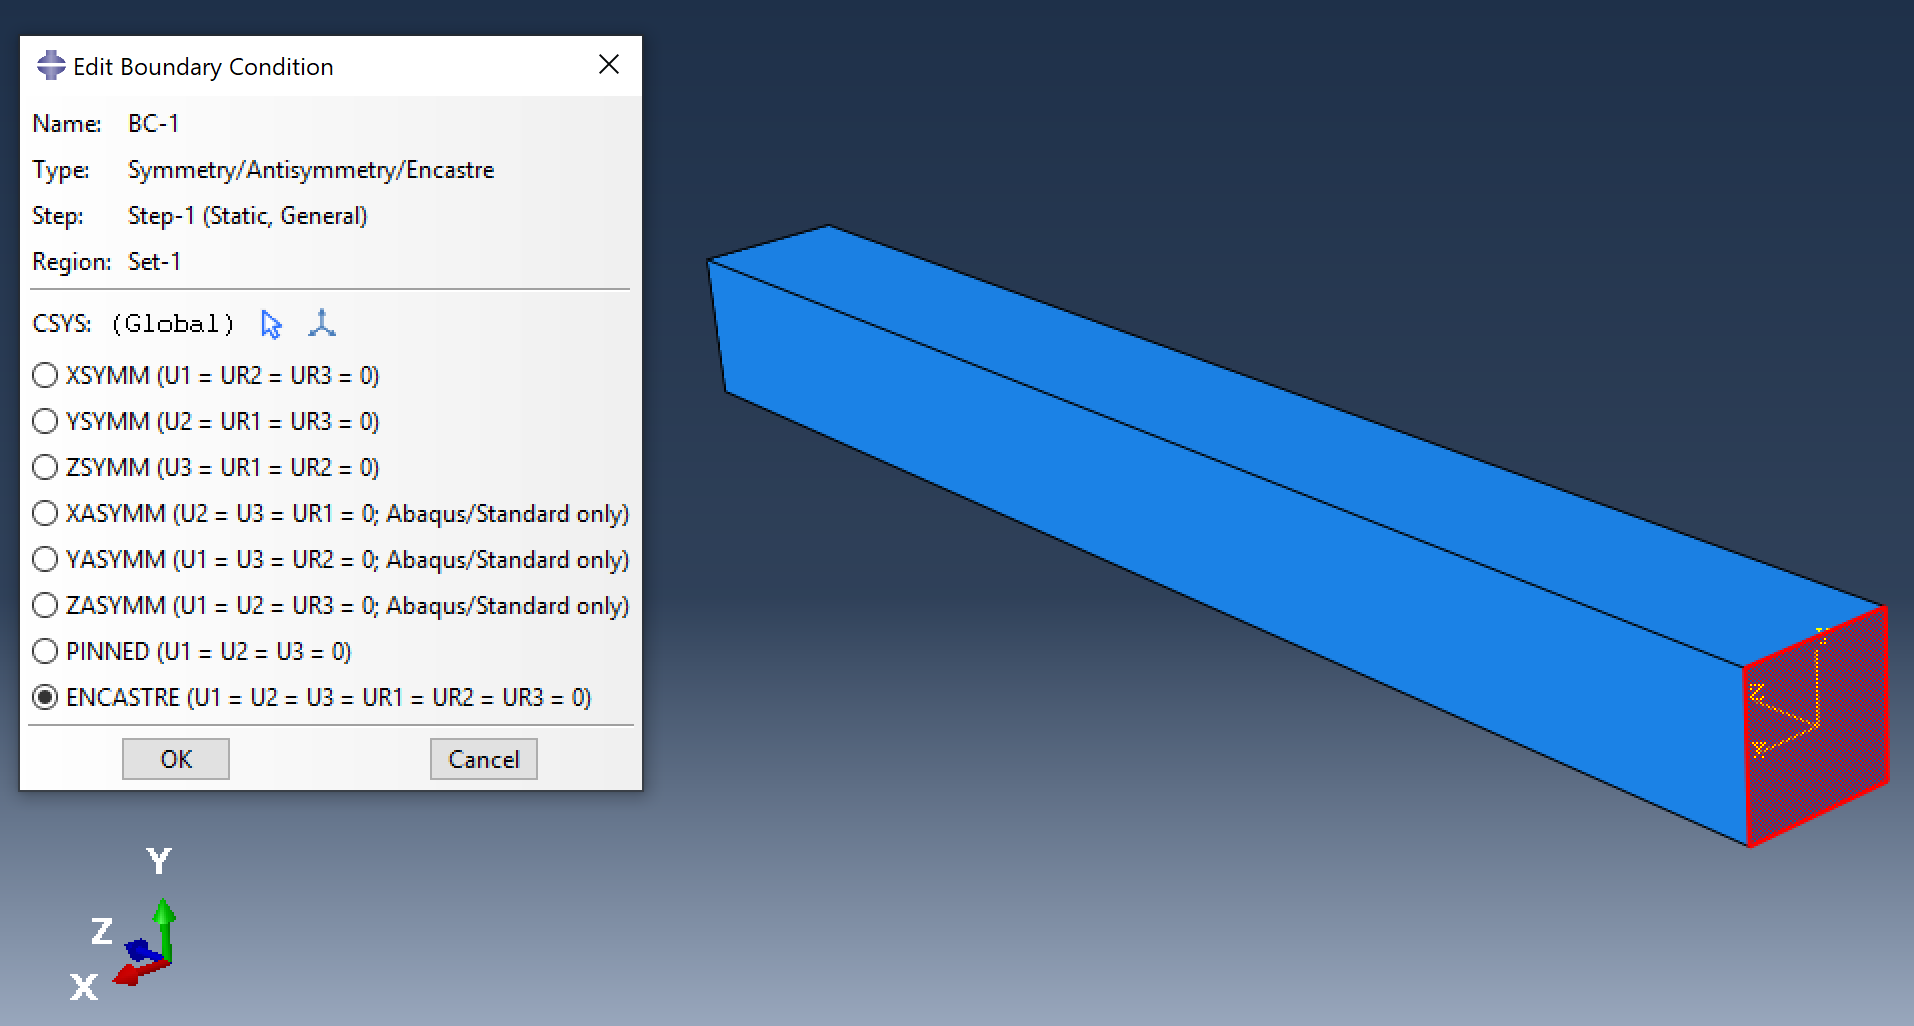
\includegraphics[scale=0.4]{capturas/load3.png}
\caption{Tipo de \emph{Boundary Condition: Encastre}}
\label{fig:load2}
\end{figure}

Pasamos entonces a definir las dos condiciones de carga que aplican en nuestro problema: carga puntual y volumétrica. Con respecto a la primera se puede realizar de diversas formas. La que consideramos más inmediata es aplicar una tracción a la superficie en \emph{Z=L}, teniendo en cuenta que en \texttt{Abaqus} es una carga de categoría \emph{Mechanical} y tipo \emph{Surface Traction} (figura \ref{fig:load3a}). Definimos a continuación la superficie donde se va a aplicar y se nos abrirá la pestaña de edición de carga (figura \ref{fig:load3b}). La carga es de distribución uniforme, y la tracción de tipo \emph{General}. Para la dirección debemos dibujar en el modelo un vector que siga la dirección creciente del eje \emph{Z}, por lo que se nos debe escribir un vector unitario (0,0,1). La magnitud  será de 5 N divivido de la superficie donde se aplica, 1 mm$^2$, es decir, 5 MPa.

\clearpage
\begin{figure}[h!tp]
\centering
\captionsetup[subfigure]{justification=centering,singlelinecheck=false}
  \begin{subfigure}[b]{0.74\textwidth}
  \hspace{0mm}
    \imagebox{75mm}{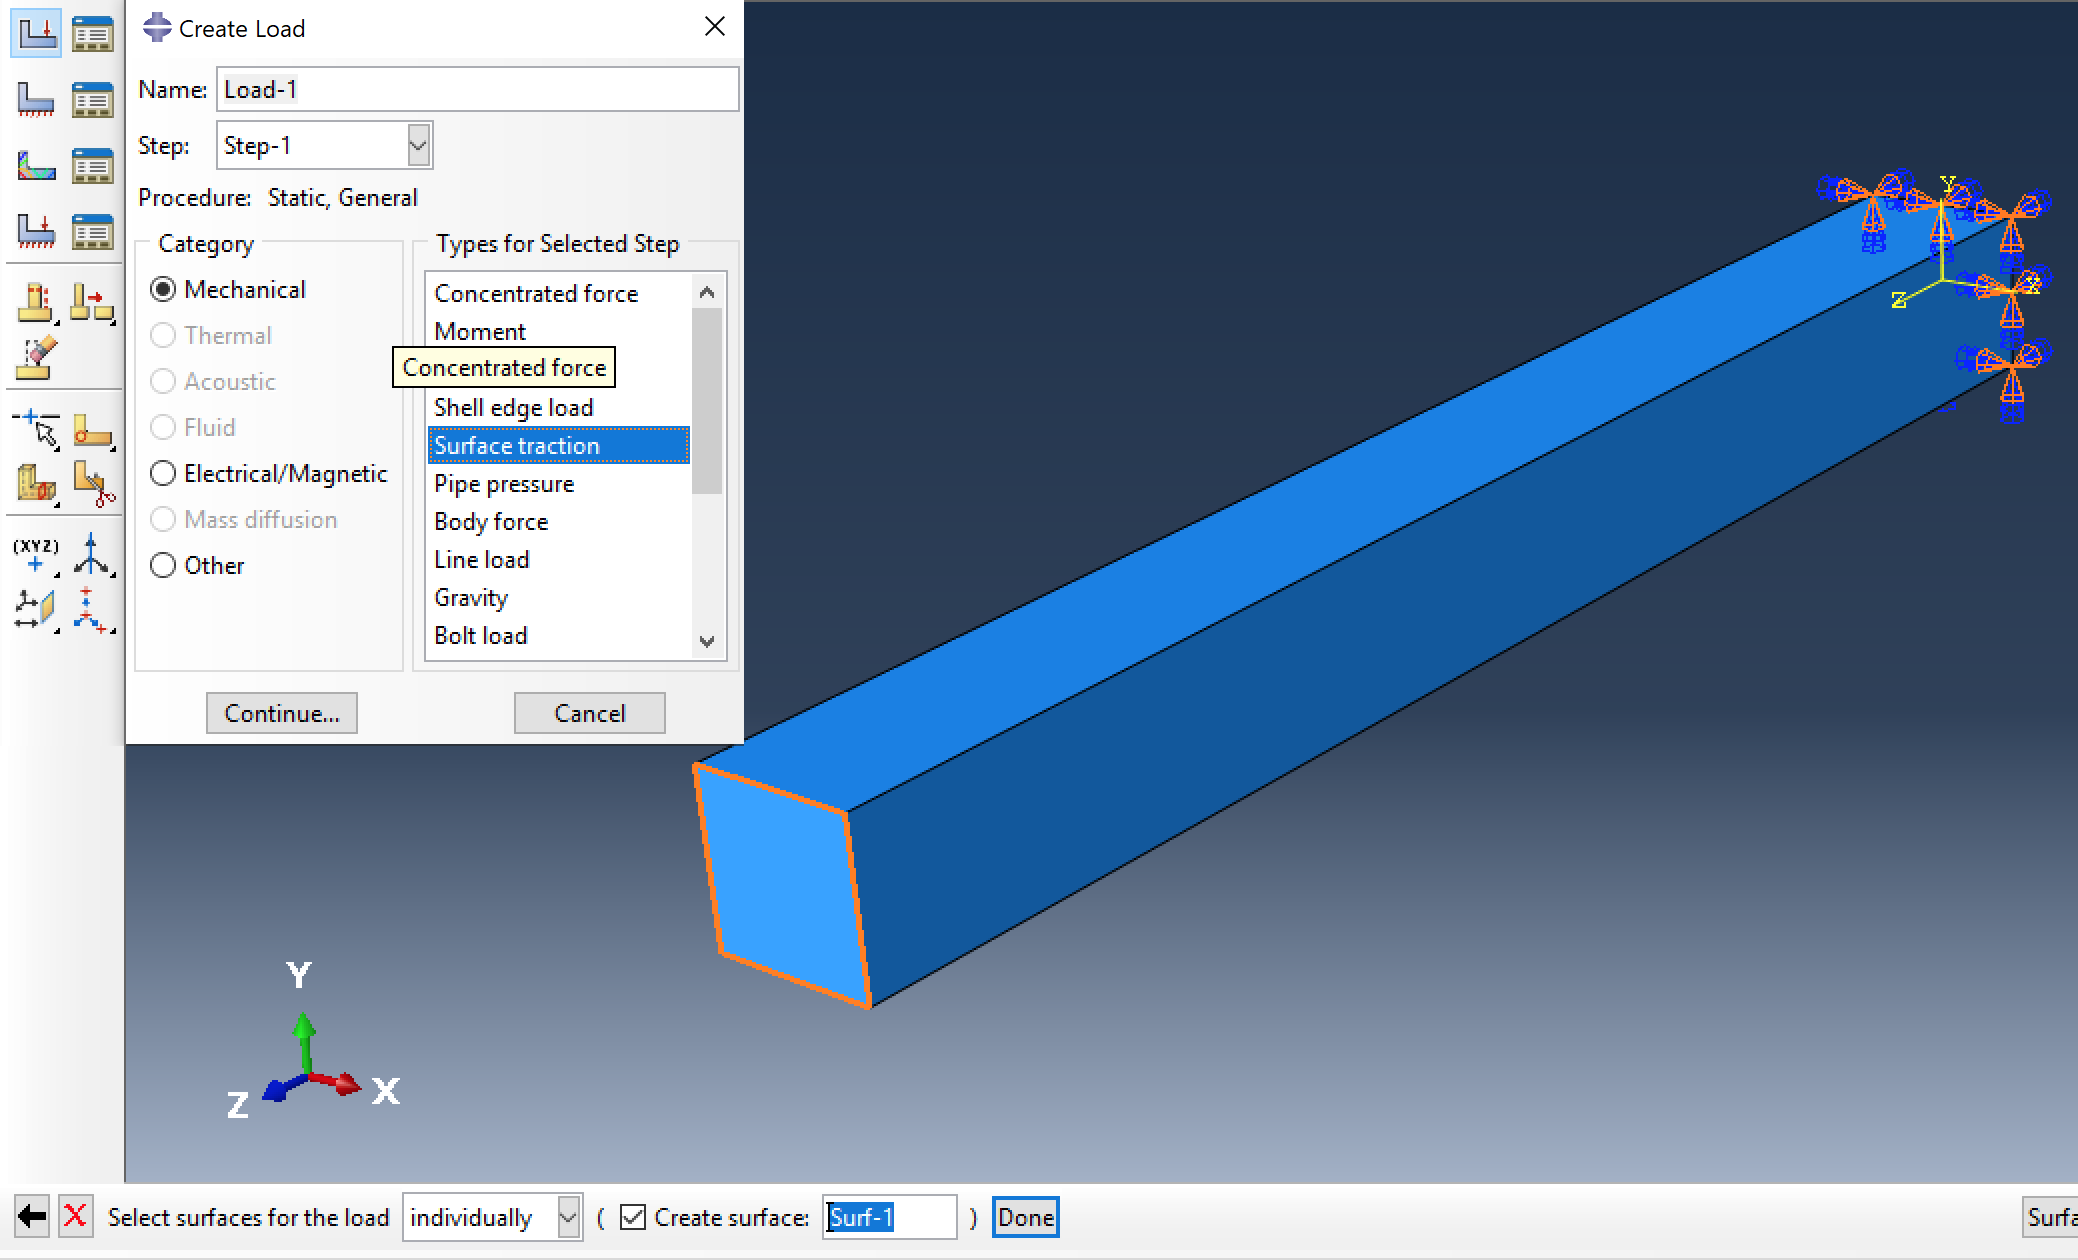
\includegraphics[scale=0.32]{capturas/load4.png}}
    \caption{Creación de la carga y asignación\label{fig:load3a}}
  \end{subfigure}
  \begin{subfigure}[b]{0.25\textwidth}
  \hspace{0mm}
    \imagebox{75mm}{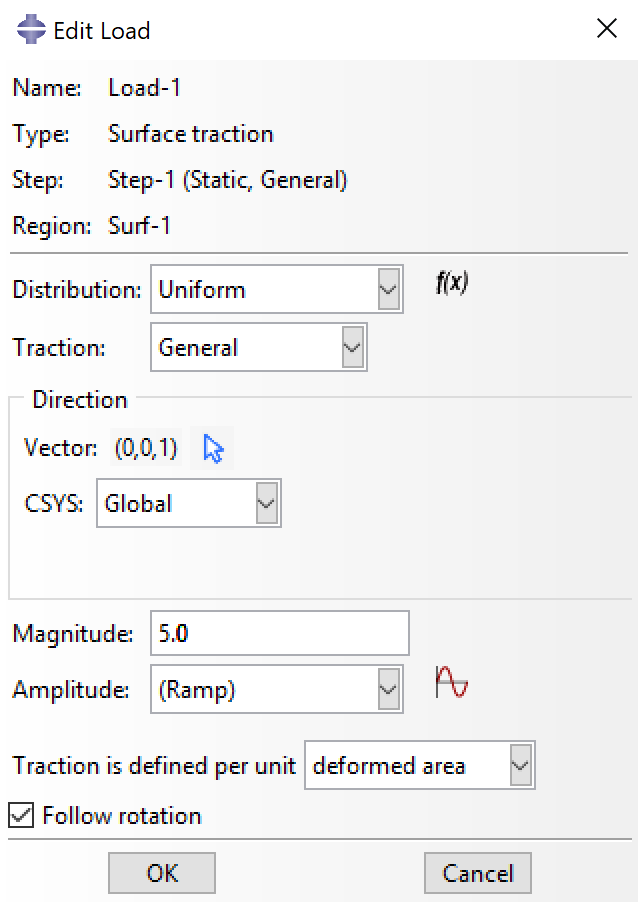
\includegraphics[scale=0.46]{capturas/load5.png}}
    \caption{Definición\label{fig:load3b}}
  \end{subfigure}
\caption{Carga puntual}
\label{fig:load3}
\end{figure}

En lo que respecta a la carga volumétrica repartida en todo el cuerpo se ha de seleccionar el tipo \emph{Body Force} en el apartado de creación de cargas y posteriormente asignarsela a todo el cuerpo (figura \ref{fig:load4}).

\begin{figure}[h!tp]
\centering
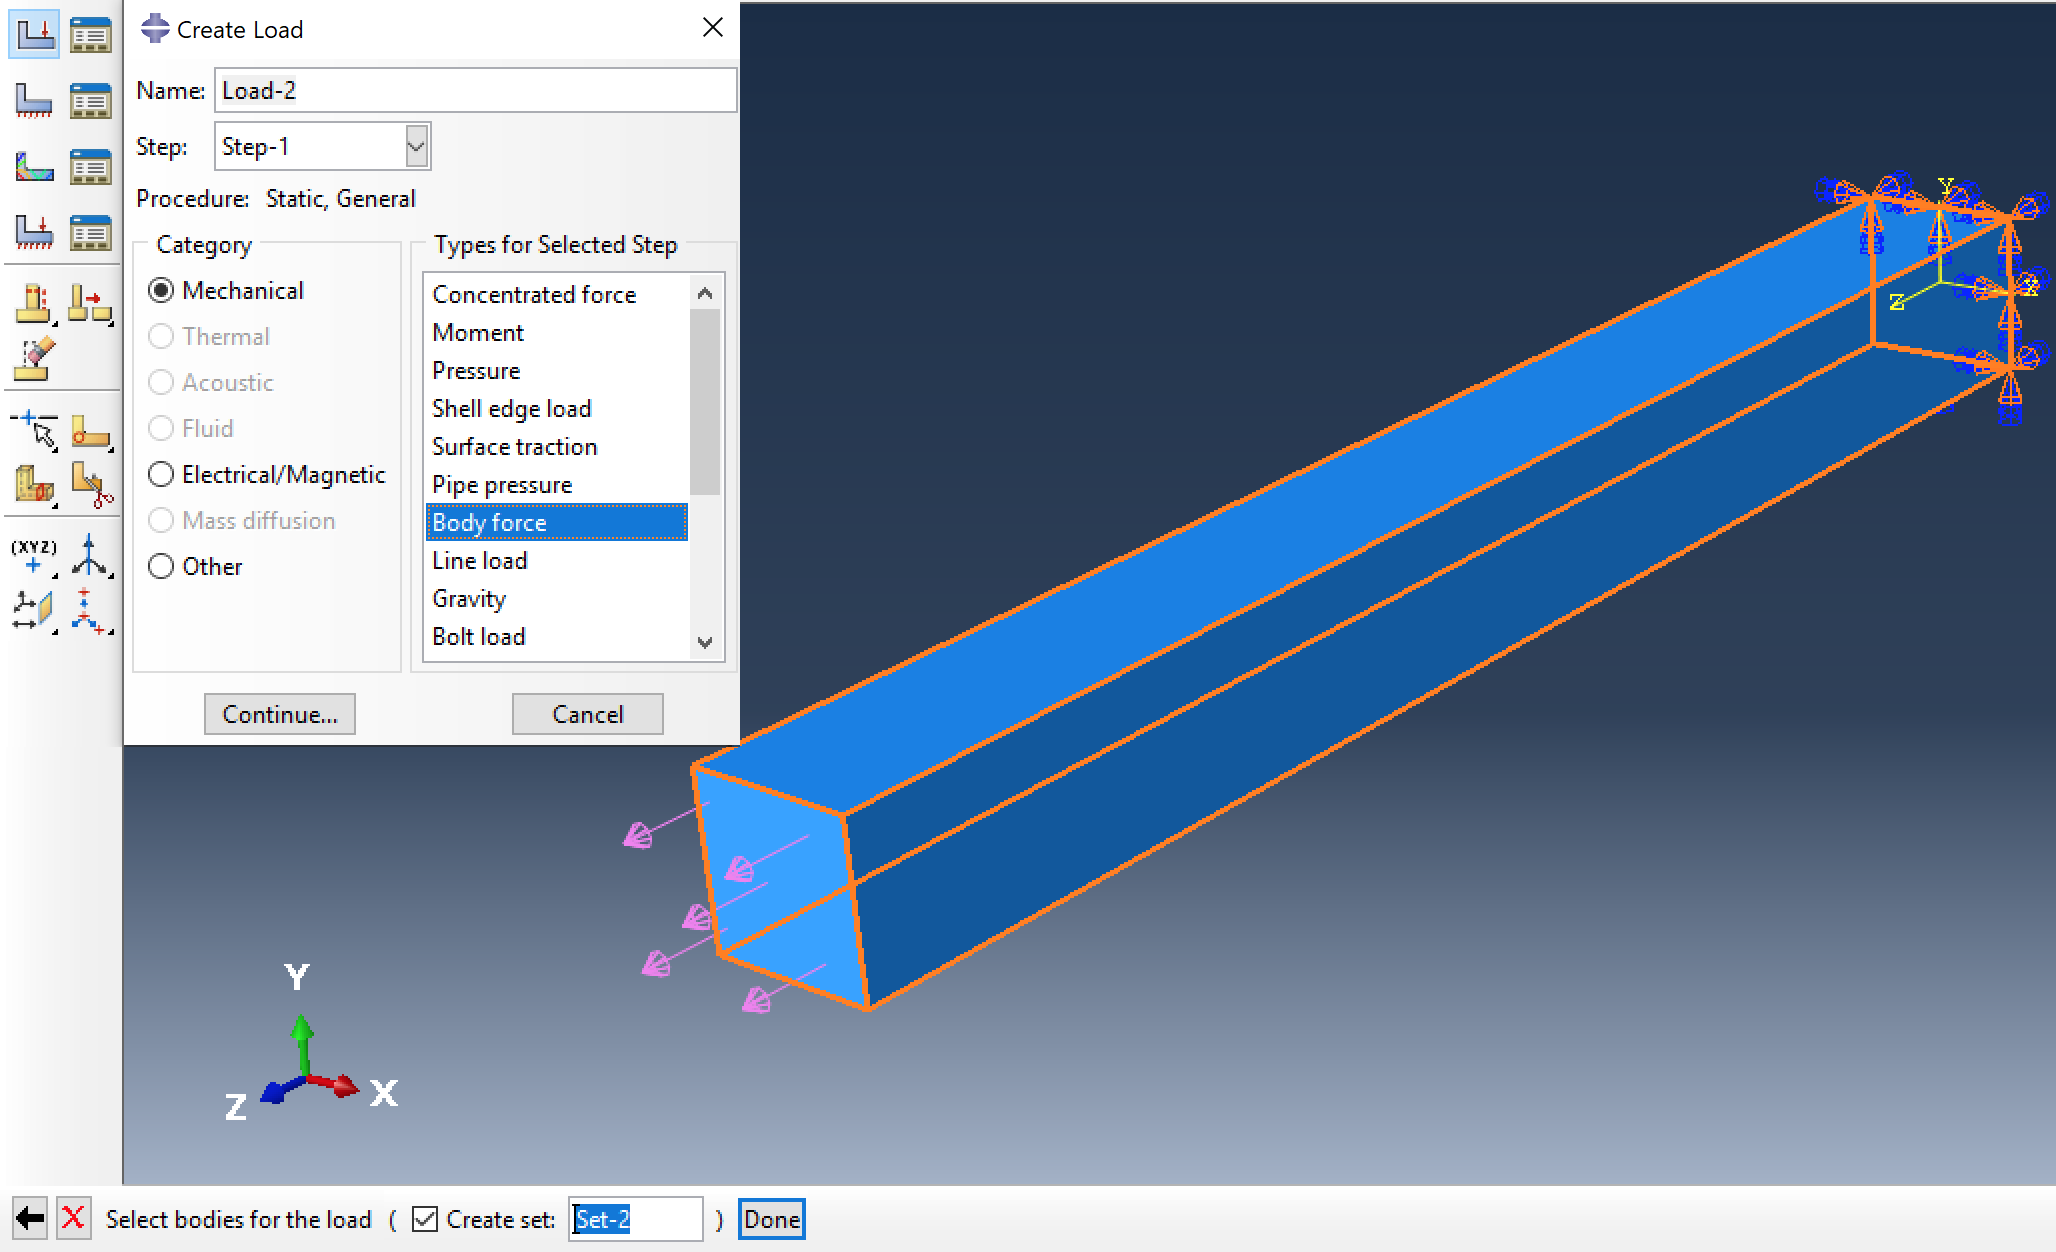
\includegraphics[scale=0.35]{capturas/load6.png}
\caption{Creación de la carga \emph{Body Force}}
\label{fig:load4}
\end{figure}

A continuación hemos de definir dicha carga. Para ello hemos de hacer clic primero en un botón con el símbolo $f(x)$, puesto que no será un valor puntual sino una función. Para la resolución de este problema optamos por asignar una expresión. Se nos abrira una ventana de creación de \emph{Expression Field}. Teniendo en cuenta que el número de  matrícula asignado en esta práctica es 1024, deberemos crear una carga que siga la ecuación $q=0.2 + 0.04*Z$, puesto que nuestra barra sigue dicha dirección en el modelo de \texttt{Abaqus}. Será esta la ecuación que deberemos escribir en el campo correspondiente. Una vez creado, en el campo \emph{Distribution}, en la ventana \emph{Edit Load}, asiganaremos el \emph{Expression Field} creado, en nuestro caso \emph{AnalyticalField-1}. La componente será la (0,0,0), es decir, siguiendo la dirección \emph{Z}.

\clearpage
\begin{figure}[h!tp]
\centering
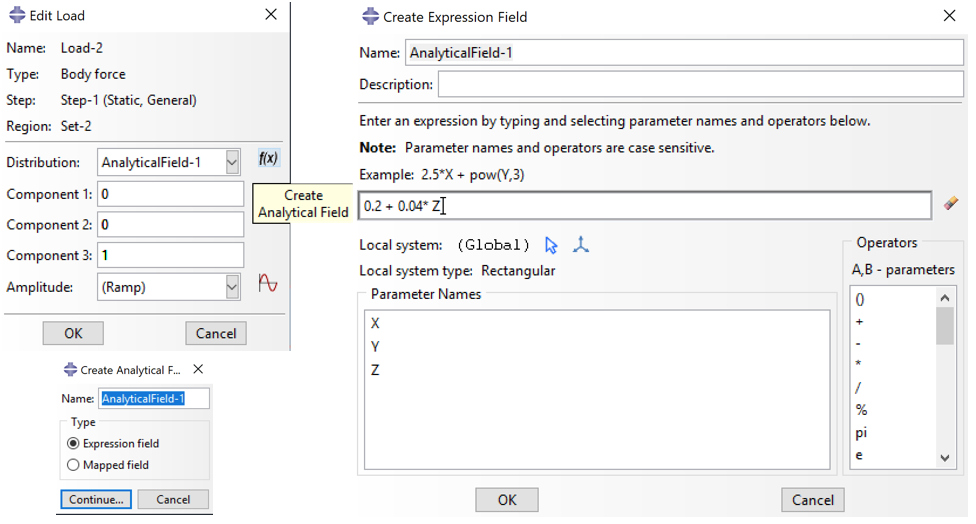
\includegraphics[scale=0.85]{capturas/load7.png}
\caption{Definición de la distribución de carga con una expresión}
\label{fig:load5}
\end{figure}

Una vez definida esta segunda carga, nuestro modelo debe tener una apariencia como la que vemos a continuación:

\begin{figure}[h!tp]
\centering
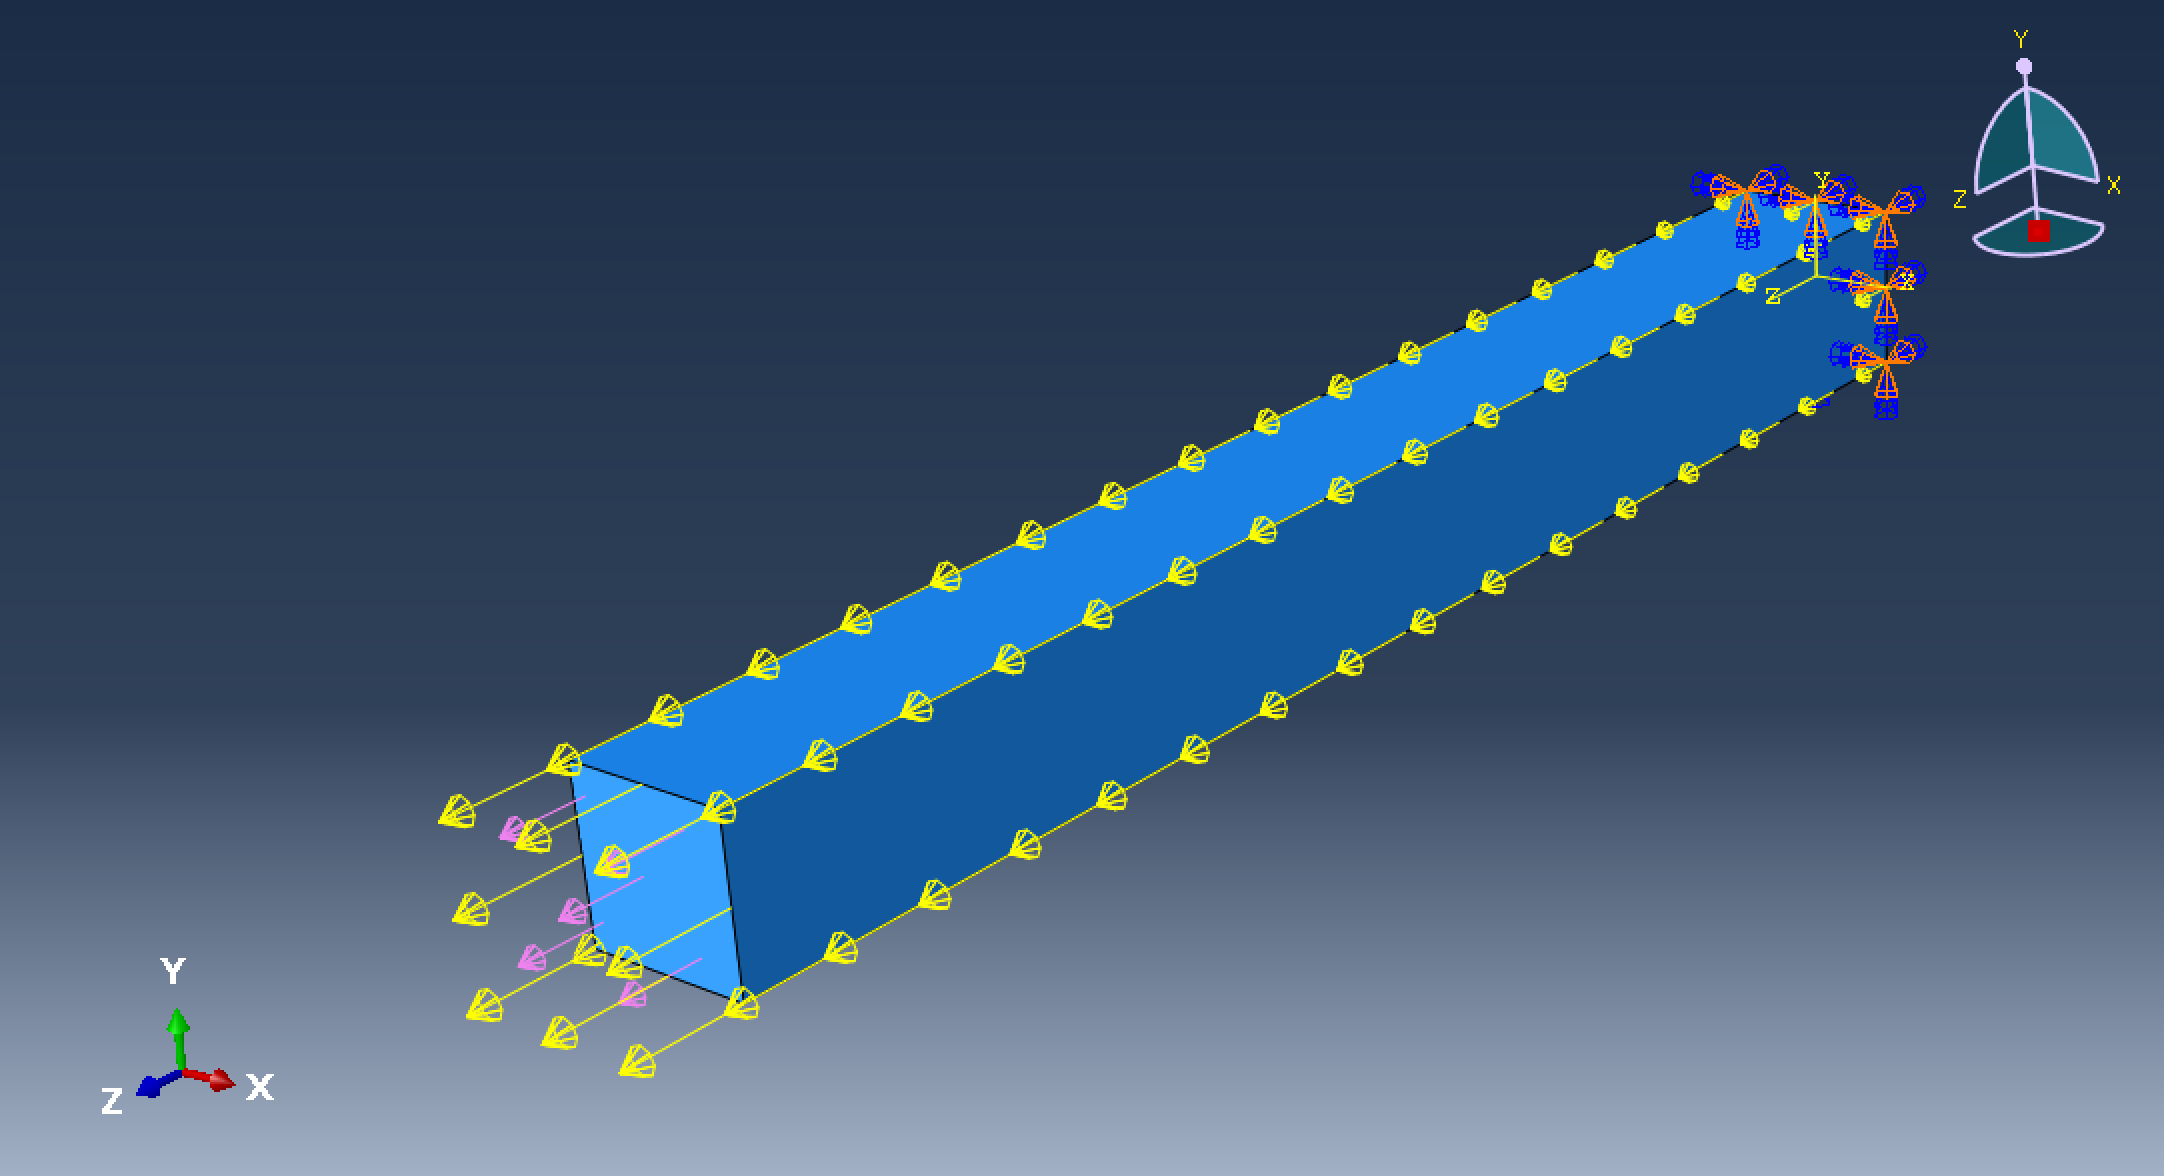
\includegraphics[scale=0.38]{capturas/load8.png}
\caption{Distribución de cargas final}
\label{fig:load6}
\end{figure}

\clearpage

\subsection{Módulo \texttt{Mesh}}
%Within the \texttt{Mesh} module, start by selecting the part by expanding the tee of the model at the left side, and activating with the right button the icon \emph{``Mesh''}:
En el módulo mesh hay que comenzar por seleccionar la parte expandiendo el árbol del modelo / parte de la izquierda, y activando con el botón derecho el icono \emph{``Mesh''}:
Fig.~\ref{fig:mesh-part}.
%Open in the top menu bar \emph{Mesh} $\to$ \emph{Controls} and select ``Hex'' and ``Structured'', to generate s structured mesh of quadrilaterals 
Se abre en el menú superior \emph{Mesh} $\to$ \emph{Controls} y se selecciona ``Hex'' y ``Structured'', para generar una malla estructurada de cuadriláteros
(Fig. \ref{fig:mesh-controls}).
\begin{figure}[h!tp]
\parbox[t]{0.49\textwidth}{%
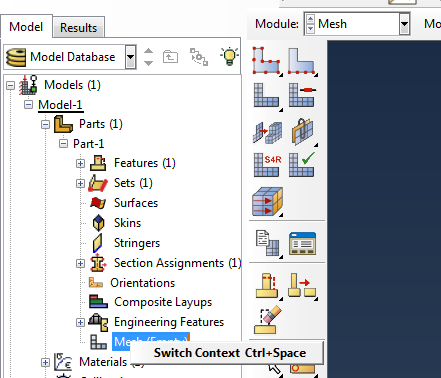
\includegraphics[width=0.5\textwidth]{capturas/29-mesh.png}
%\caption{Expanded model tree for mesh.}
\caption{Seleccionar en el menú desplegado del modelo para mallar.}
\label{fig:mesh-part}%
}\quad
\parbox[t]{0.49\textwidth}{%
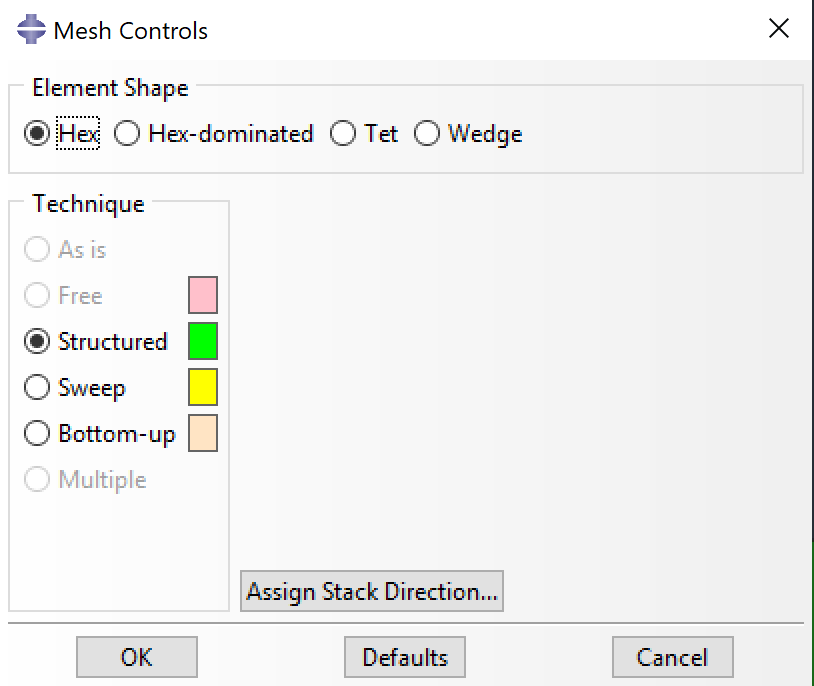
\includegraphics[width=0.5\textwidth]{capturas/30-mesh-x.png}
%\caption{Define options in ``Mesh controls''}
\caption{Definir opciones en ``Mesh controls''}
\label{fig:mesh-controls}%
}%
\end{figure}

%Following, open in the top bar the menu \emph{Mesh} $\to$ \emph{Element type} and select the options \emph{``3D stress''}, \emph{``Membrane stress: Linear''}, \emph{``Reduced integration''} which will correspond to element type C3D8R, enough for the involved calculation
A continuación se abre en el menú superior \emph{Mesh} $\to$ \emph{Element type} y se seleccionan las opciones ``3D Stress'', ``Linear'', \emph{``Reduced integration''} lo que dará lugar al elemento C3D8R, suficiente para el cálculo que vamos a realizar. 
(Fig. \ref{fig:mesh-element}).
\begin{figure}[h!tp]
\centering
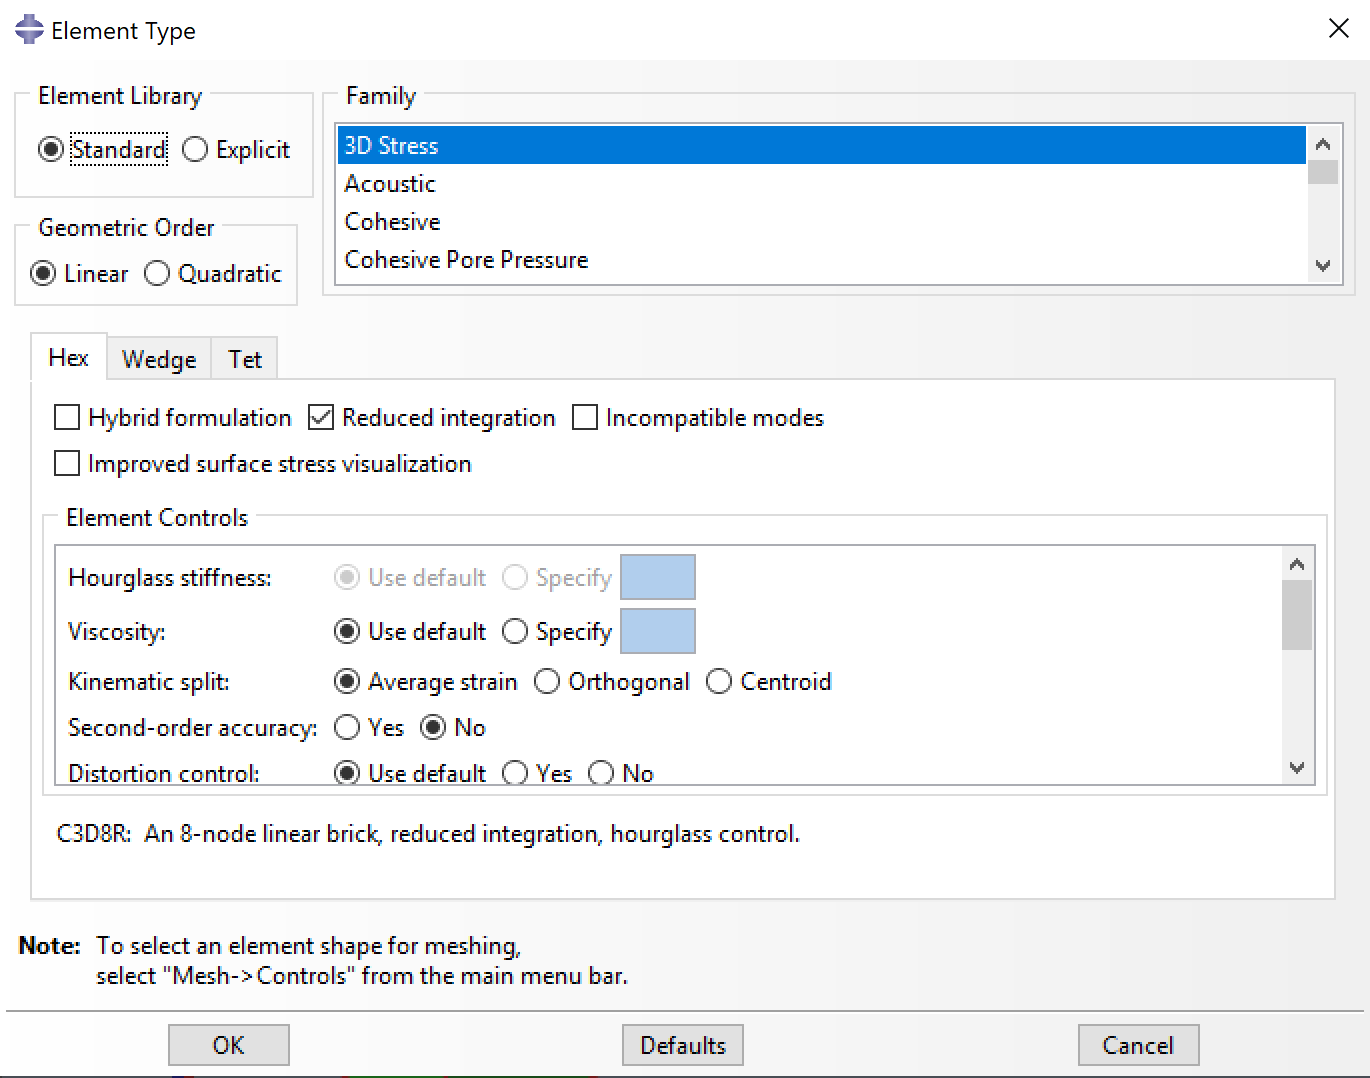
\includegraphics[scale=0.4]{capturas/31-mesh.png}
\caption{Seleccionar tipo de elemento en ``Mesh/element''}
\label{fig:mesh-element}%
\end{figure}

El tamaño \emph{``Semilla''} que vamos a emplear es de 1 mm en todas las direcciones del espacio, teniendo en cuenta queremos realizar un mallado de 10 elementos hexaedrícos en la dirección longitudinal de la barra (Fig. \ref{fig:mesh1}).

\clearpage
\begin{figure}[h!tp]
\centering
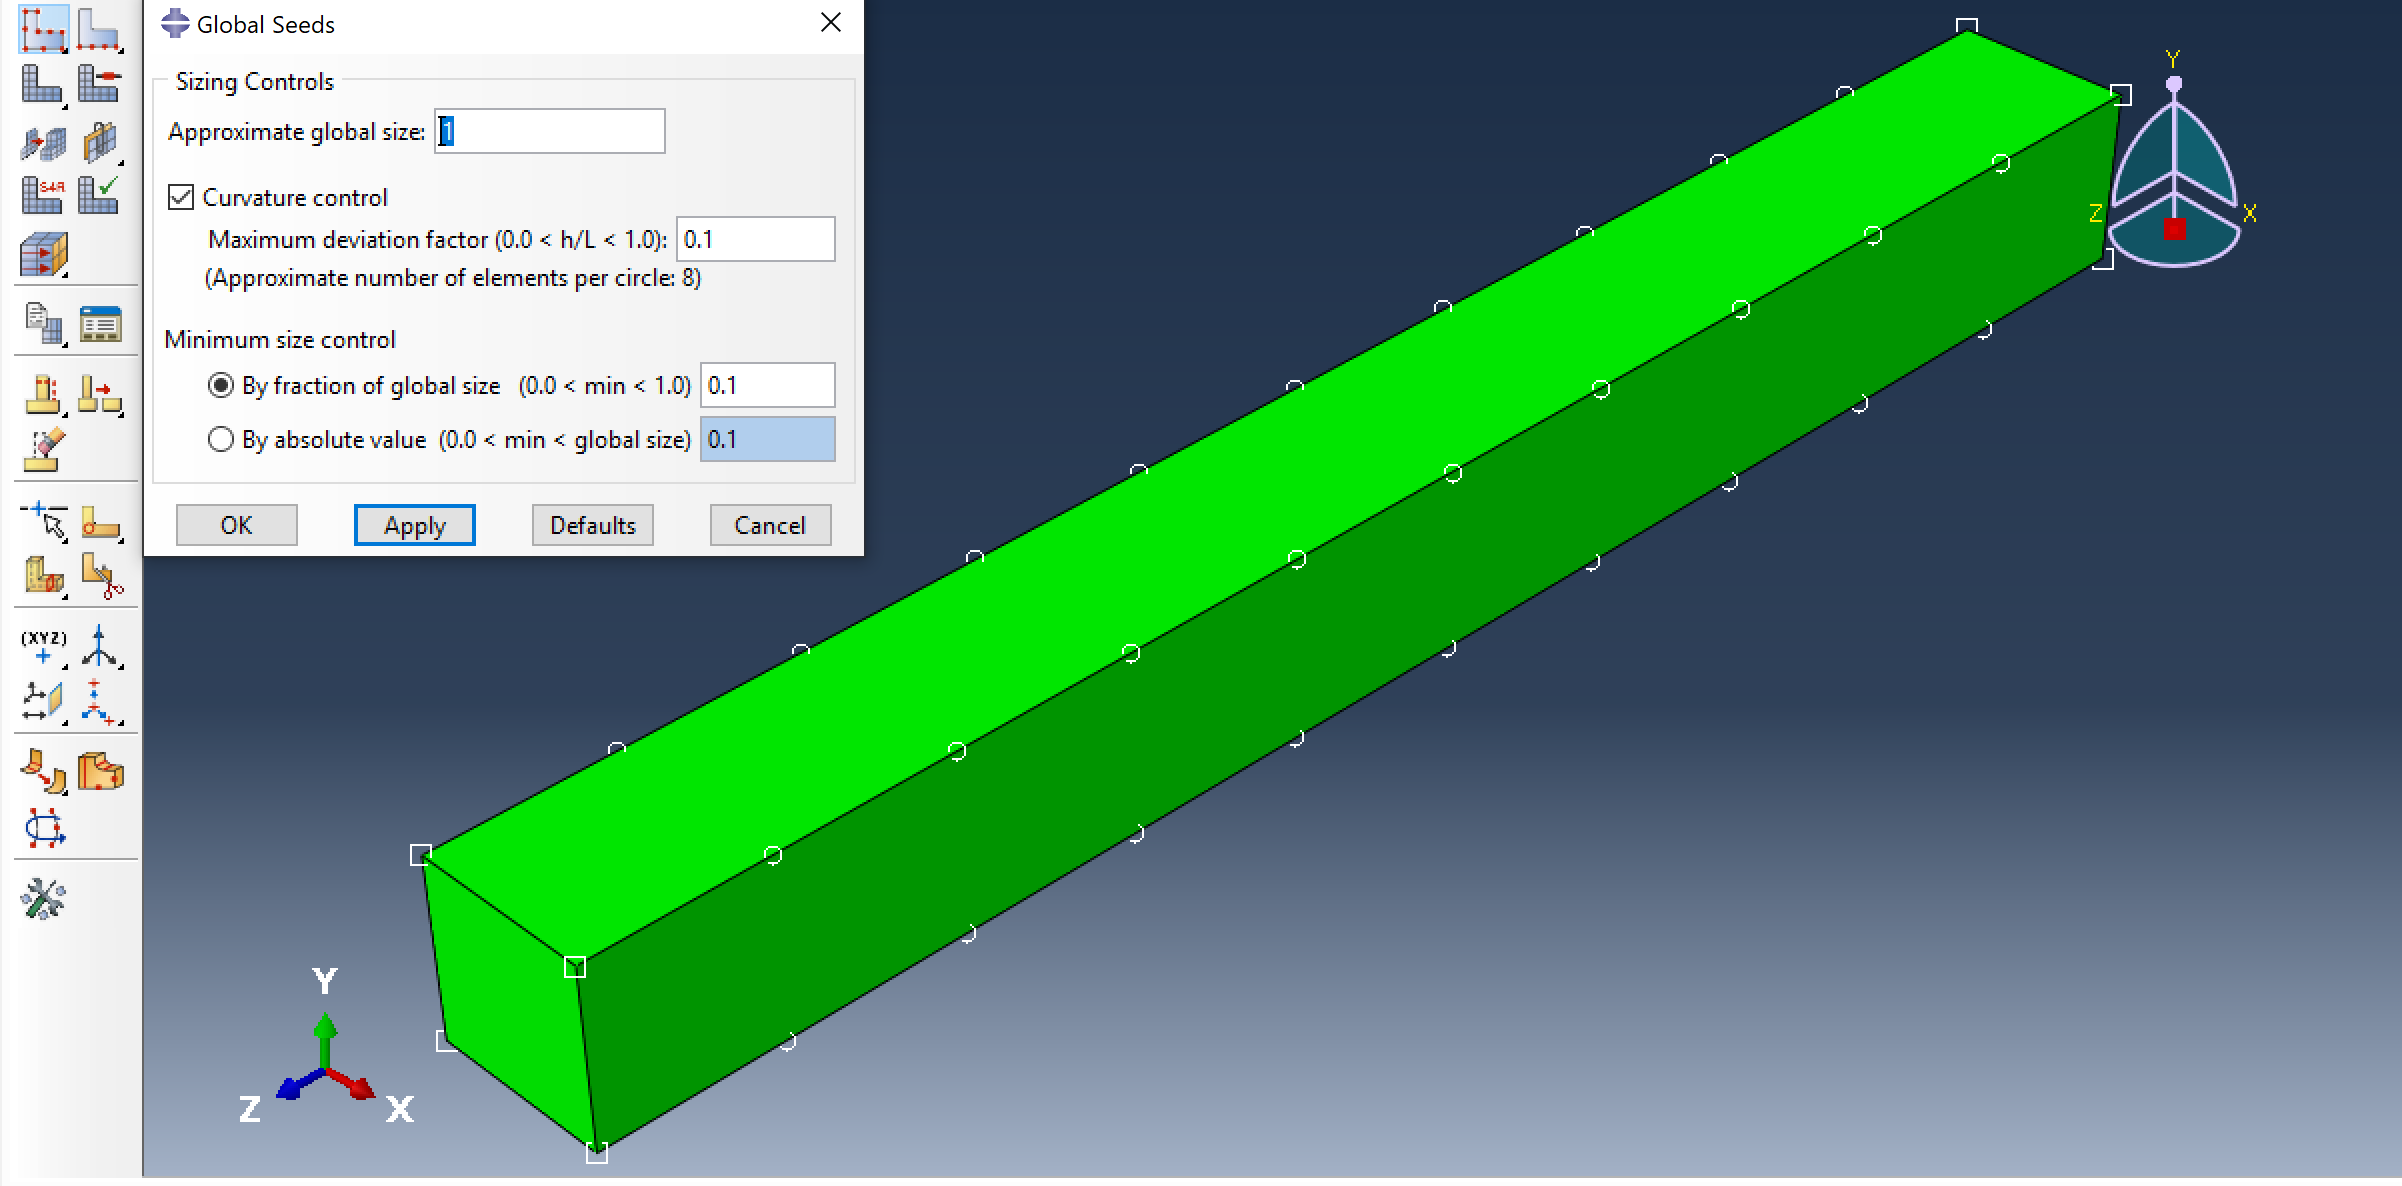
\includegraphics[scale=0.4]{capturas/mesh1.png}
\caption{``Global Seeds'' empleado}
\label{fig:mesh1}%
\end{figure}

Por tanto, la malla que resulta es la que vemos a continuación

\begin{figure}[h!tp]
\centering
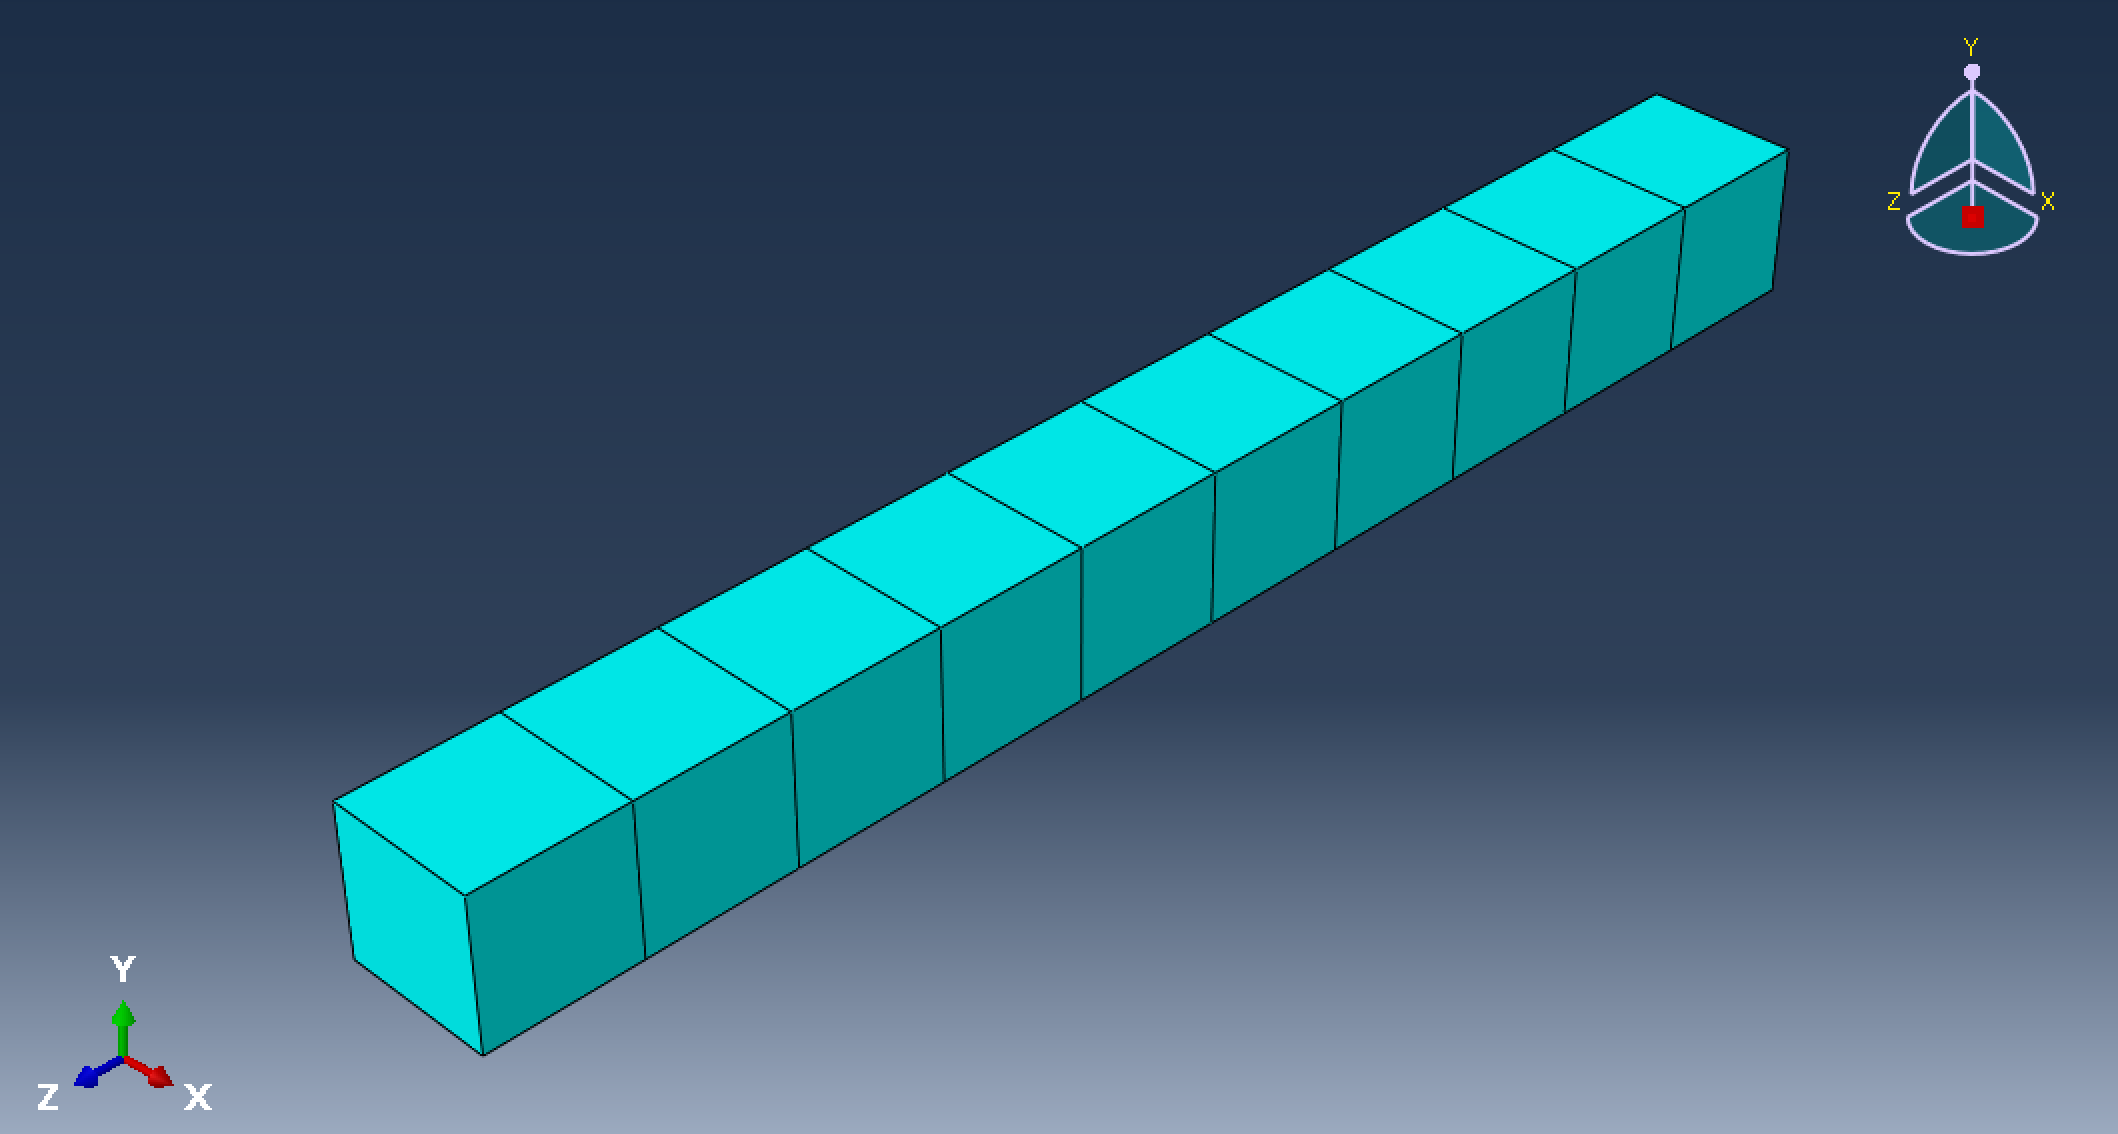
\includegraphics[scale=0.4]{capturas/mesh2.png}
\caption{Malla obtenida}
\label{fig:mesh2}%
\end{figure}

\clearpage
\subsection{Módulo \texttt{Job}}

Una vez completado el modelo, se crea un ``Job'' con las opciones por defecto
(figura \ref{fig:job-create}).
\begin{figure}[h!tp]
\centering
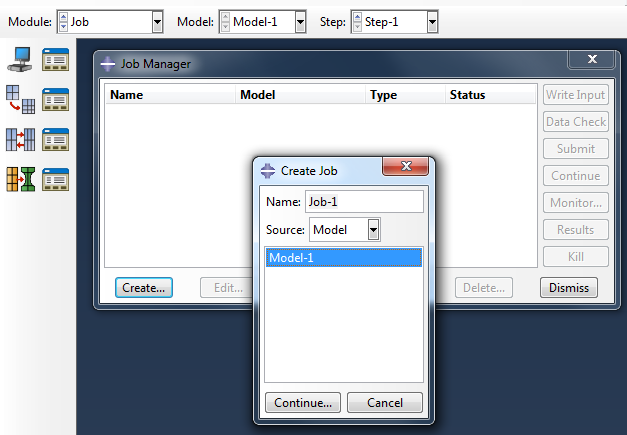
\includegraphics[scale=0.5]{capturas/37-job.png}
\caption{Creación del ``Job''}
\label{fig:job-create}
\end{figure}

Y se envía para calcular mediante ``Submit''. El \emph{Status} va cambiando de ``Submitted'' $\to$ ``Running'' $\to$ ``Completed''. 
(figura \ref{fig:job-submit})
\begin{figure}[h!tp]
\centering
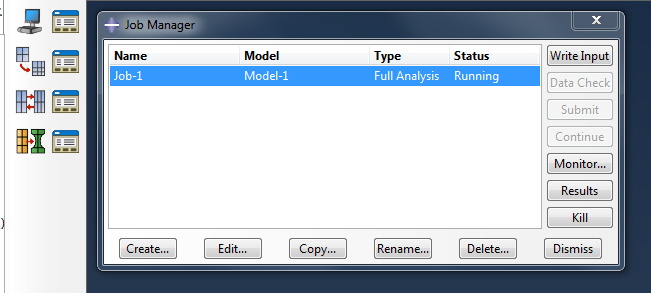
\includegraphics[scale=0.5]{capturas/38-job.png}
\caption{Envío del ``Job''}
\label{fig:job-submit}
\end{figure}
Si no hay mensaje de error el problema está acabado y se pasa al módulo de visualizar los resultados.

\clearpage
\subsection{Módulo \texttt{Visualization}}
A modo de comprobación, el primer campo a visualizar es el del desplazamiento en Z. Vemos que el desplazamiento máximo es de 0.073 mm(figura \ref{fig:U}). Vamos a dibujar la distribución del desplazamiento con respecto a la posición en \emph{Z}. 

\begin{figure}[h!tp]
\centering
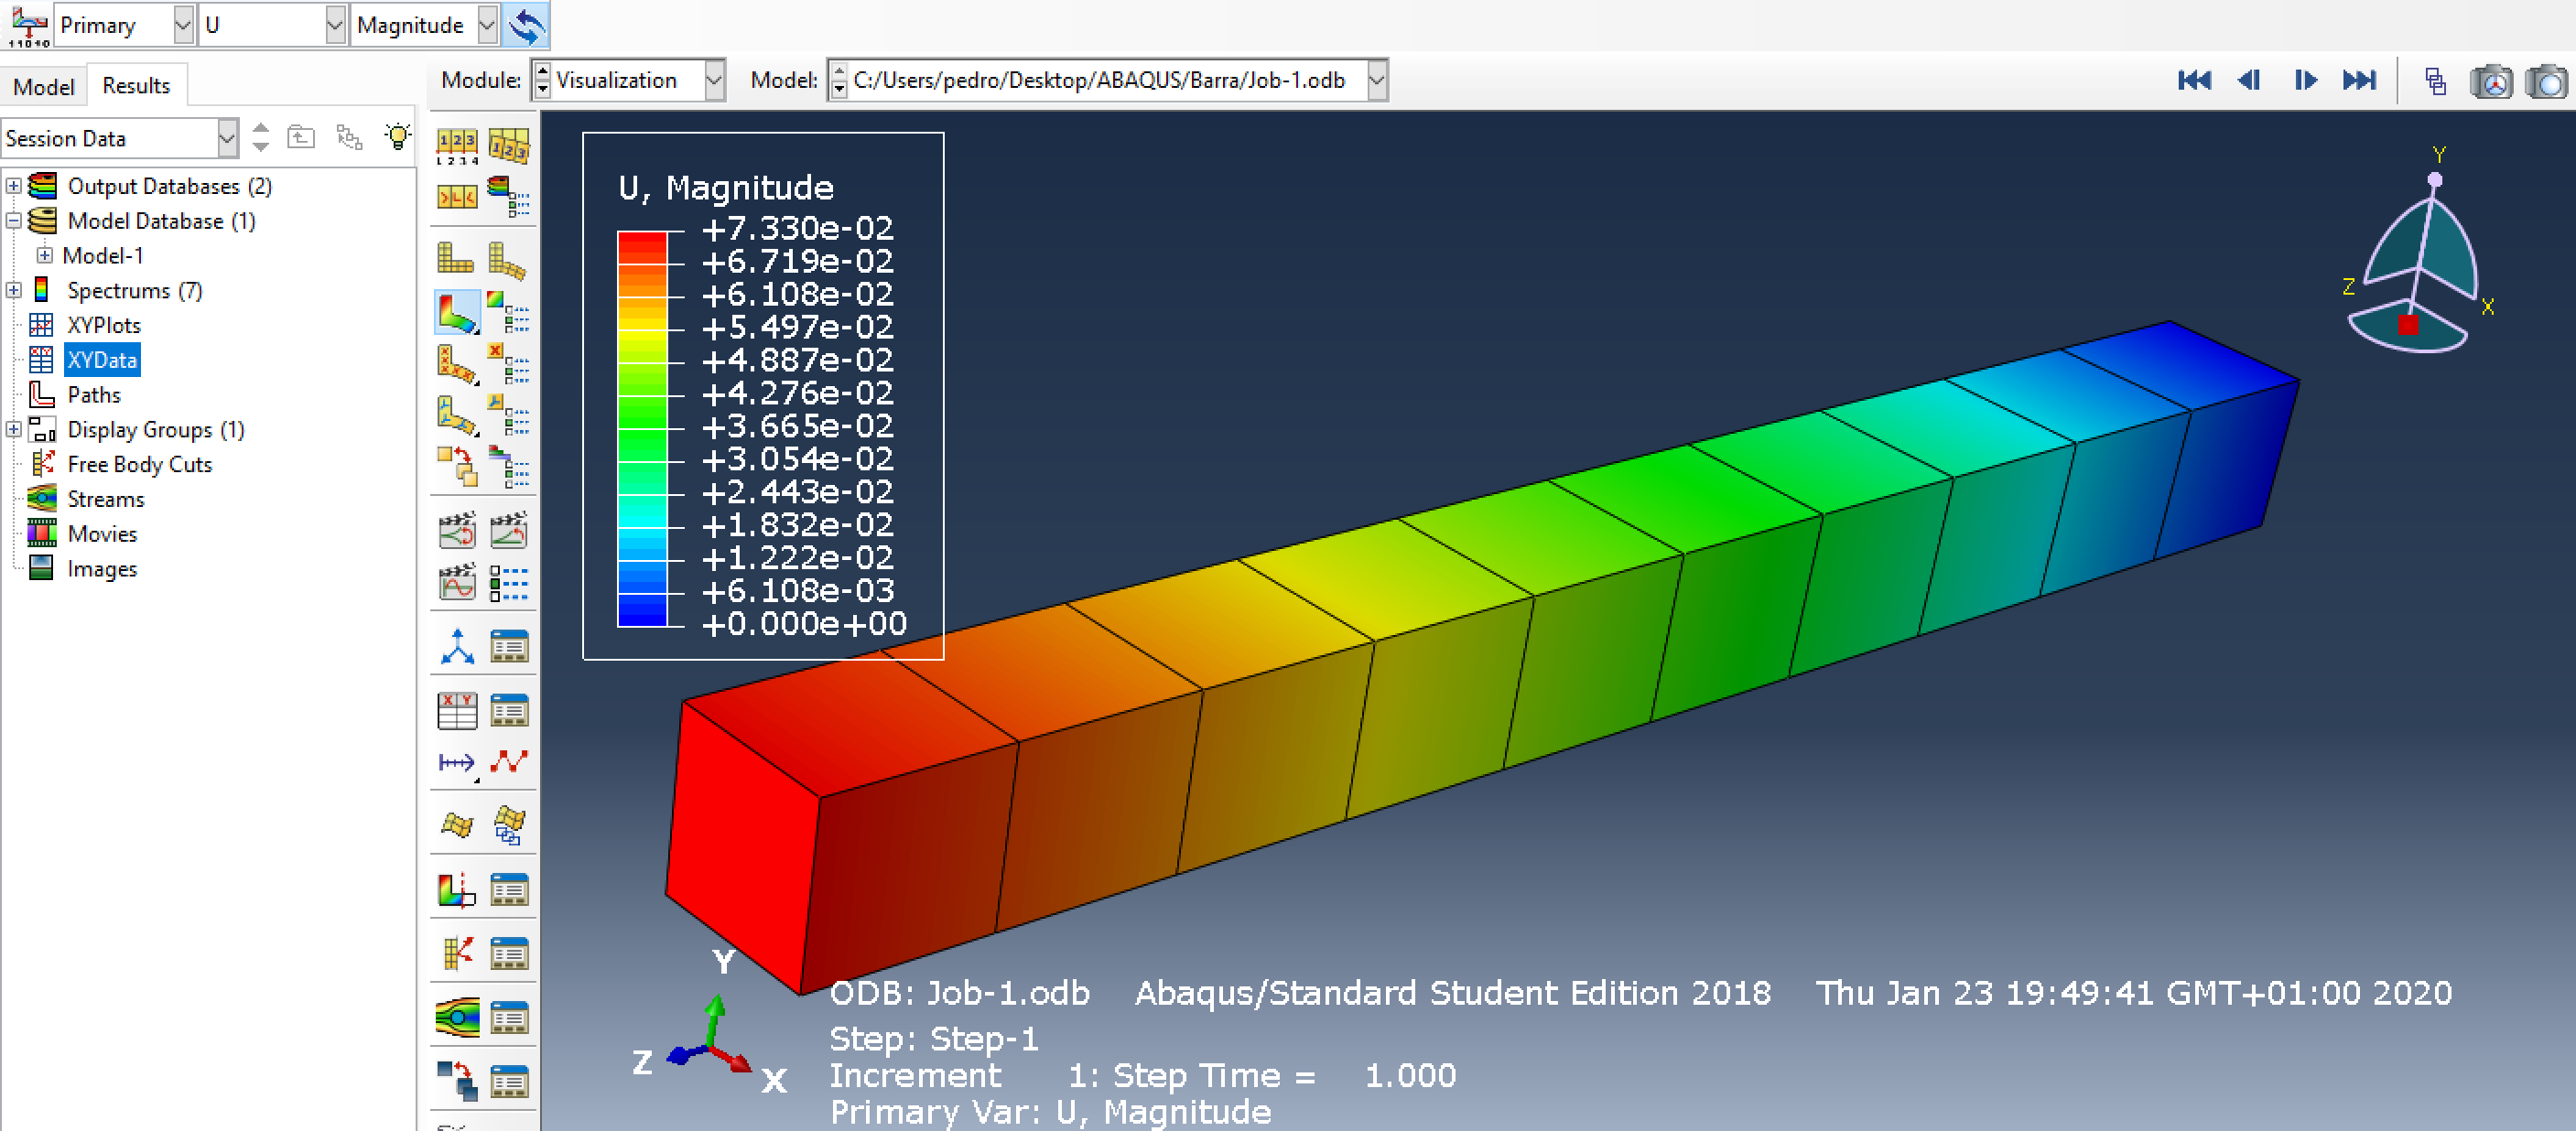
\includegraphics[scale=0.35]{capturas/res1.png}
\caption{Campo de desplazamientos}
\label{fig:U}%
\end{figure}

Antes de nada hemos de indicar un \emph{Path} que tenga nodos distribuidos en \emph{Z}. Para ello seleccionamos path y con el boton derecho abrimos un desplegable donde debemos seleccionar \emph{create} (figura \ref{fig:path}). Nuestro tipo de path será creado seleccionándolos de una lista de nodos. Nuestro modo de selección será según avanzamos en el eje Z, por lo que seleccionamos \emph{Add After} y debemos cuidar de escoger primero un nodo en $Z=0$ y el siguiente nodo en $Z=L$. Podemos elegir cualquier arista, pues todas poseen la misma información. Como queda este path definido puede verse en la figura \ref{fig:path2}.

\begin{figure}[h!tp]
\centering
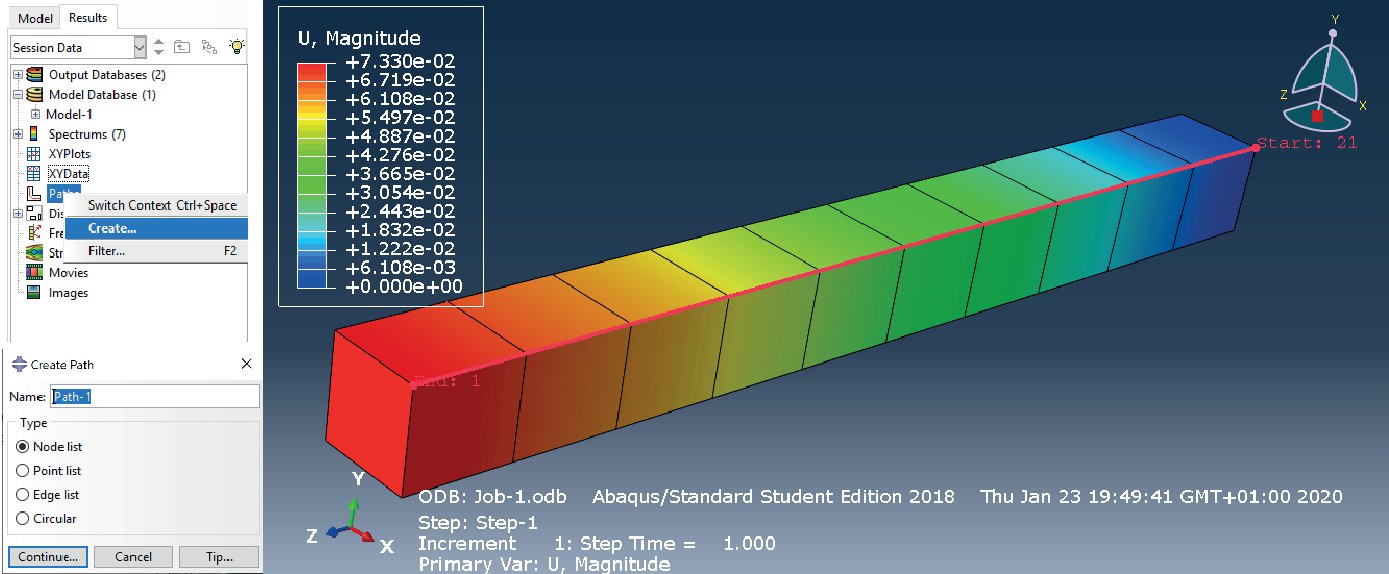
\includegraphics[scale=0.75]{capturas/path.pdf}
\caption{Definición de un path}
\label{fig:path}%
\end{figure}
\clearpage

\begin{figure}[h!tp]
\centering
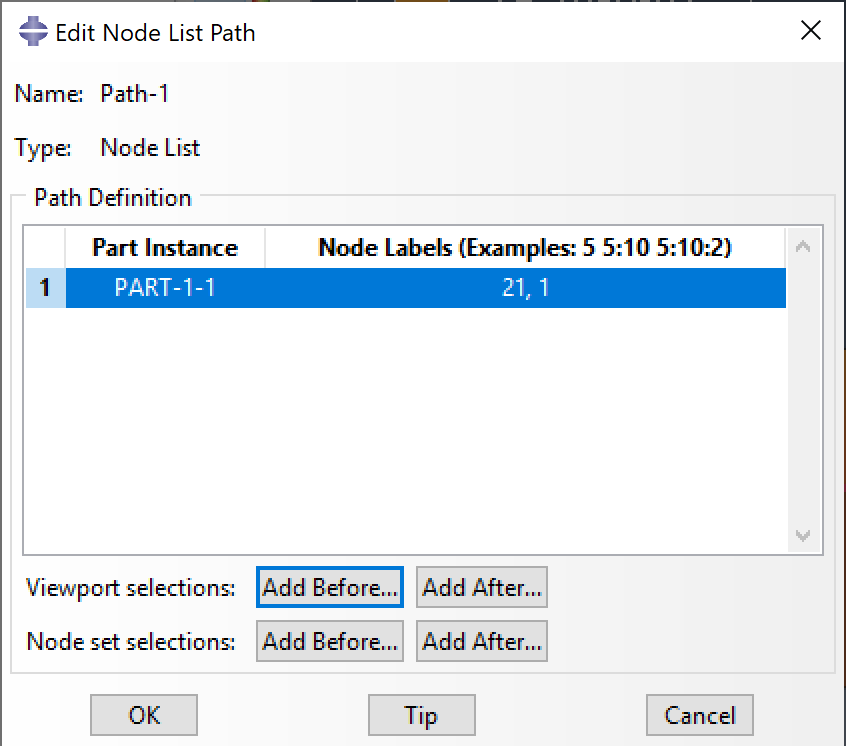
\includegraphics[scale=0.55]{capturas/path2.png}
\caption{Lista de nodos de un path}
\label{fig:path2}%
\end{figure}

Ya es posible crear un gráfico del desplazamiento en Z a lo largo de la barra. Para ello, necesitamos crear un \emph{XY-Data}. En dicho campo, con el boton derecho se nos abre un desplegable donde, al seleccionar \emph{Create}, podemos cread dicho \emph{XY-Data} desde el un Path ya definido. En nuestro caso el campo ha de ser el desplazamiento en \emph{Z, U3}. Con este campo selecionado debemos, en la ventana \emph{XY Data from Path} (figura \ref{fig:Data1}), selecionar el Path creado anteriormente (en su configuración no deformada) y selecionar la opción de incluir las intersecciones, para añadir así los valores de los nodos intermedios. Finalmente, optamos por elegir, como valor en X de nuestro gráfico, la coordenada Z.

\begin{figure}[h!tp]
\centering
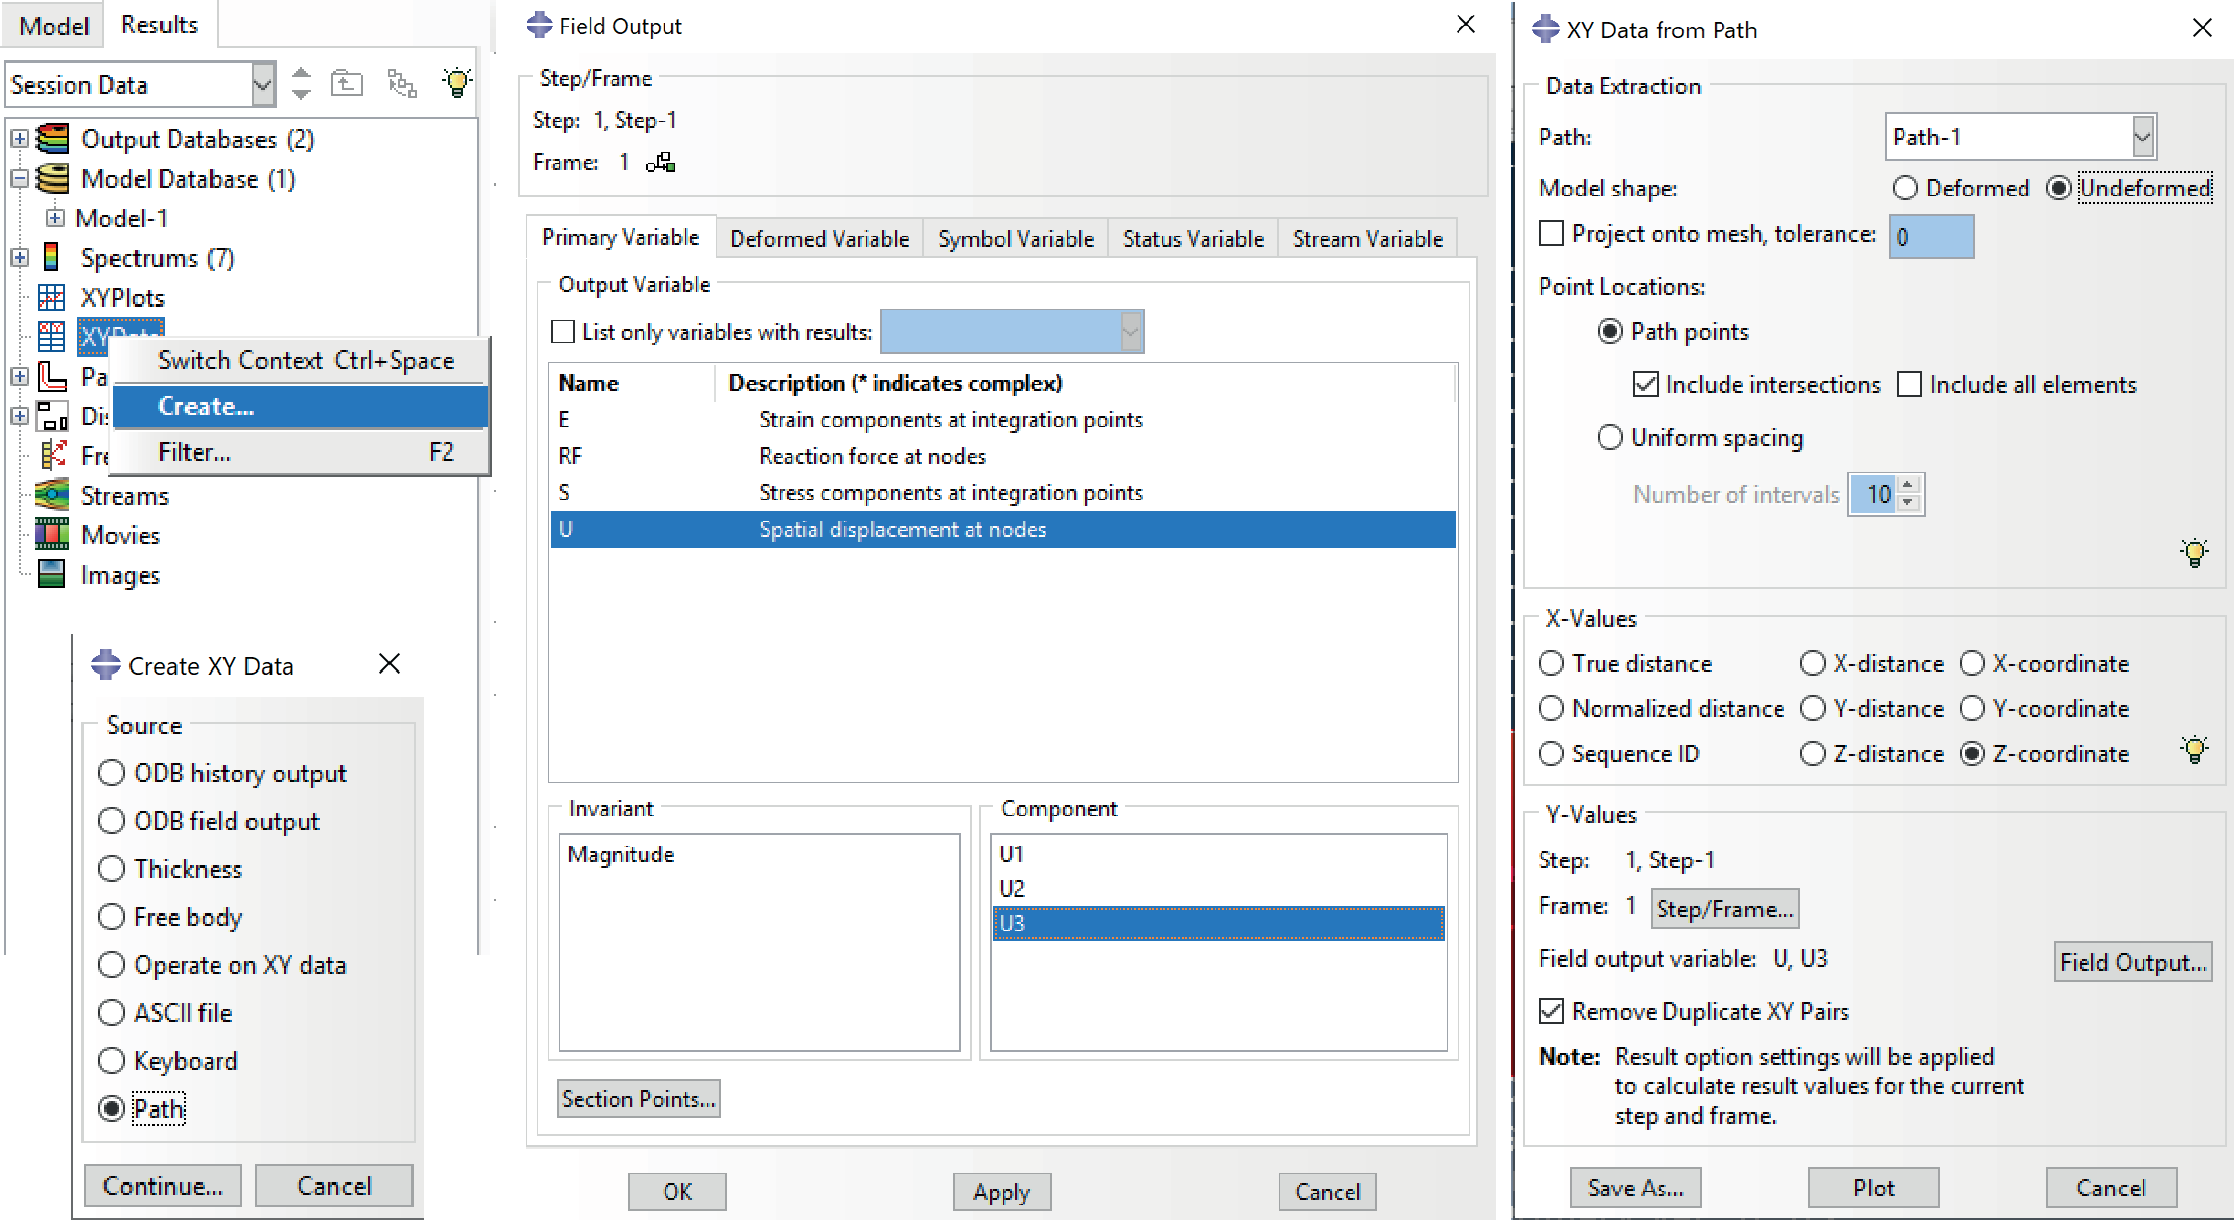
\includegraphics[scale=0.45]{capturas/U-data.pdf}
\caption{Creación de un XY-data}
\label{fig:Data1}%
\end{figure}

Si dibujamos dicho gráfico obtenemos una figura similar a la que se puede ver en la  figura \ref{fig:Data2}. Compararemos la forma y valores de esta gráfica con la que obtendremos en en \texttt{Python} para ver la correspondencia entre ambos resultados, si bien necesitaremos superponer ambas gráficas.
\clearpage
\begin{figure}[h!tp]
\centering
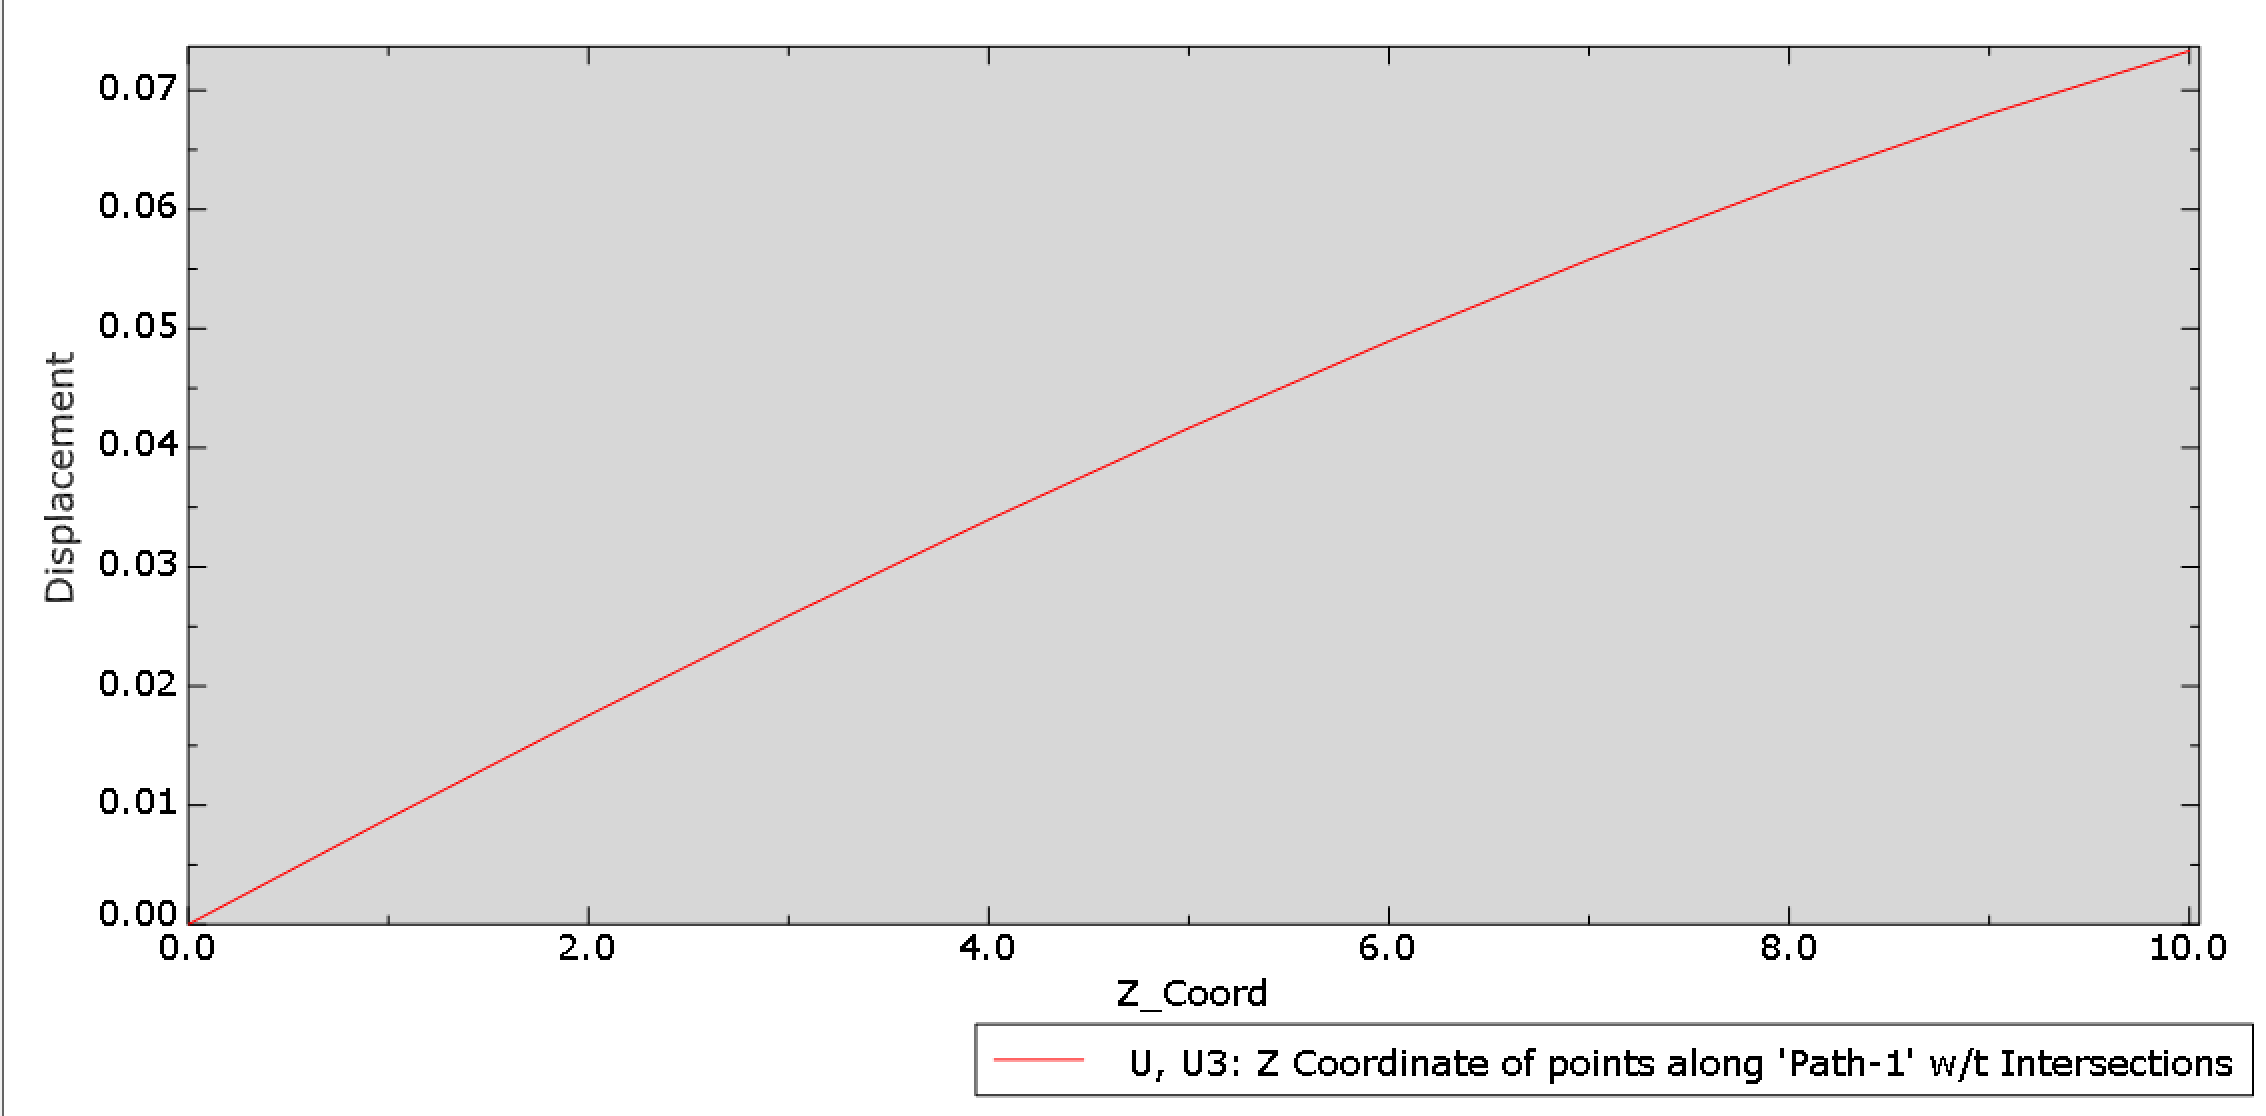
\includegraphics[scale=0.45]{capturas/U-data2.png}
\caption{Desplazamiento en en eje Z}
\label{fig:Data2}%
\end{figure}

Podemos guardar estos datos, para posteriormente exportarlos a \texttt{Python} para su comparativa con la solución analítica, haciendo clic en el botón \emph{Save as..}. El archivo de las deformaciones lo denominaremos \texttt{u3.txt}. Si intentasemos cambiar el campo de dibujo al de las tensiones, en este caso S33 que es la que se corresponde con $\sigma_z$, observamos, en la figura \ref{fig:Data3}. En cambio, aunque la tendencia y valores son cercanos, en los extremos ocurren cosas raras. Esto se debe a que la tensión es un dato correspondiente a los puntos de integración, no a los nodos, que es donde se puede hacer este path. Por tanto, para la comparativa, deberemos extraer los datos de otra manera.

\begin{figure}[h!tp]
\centering
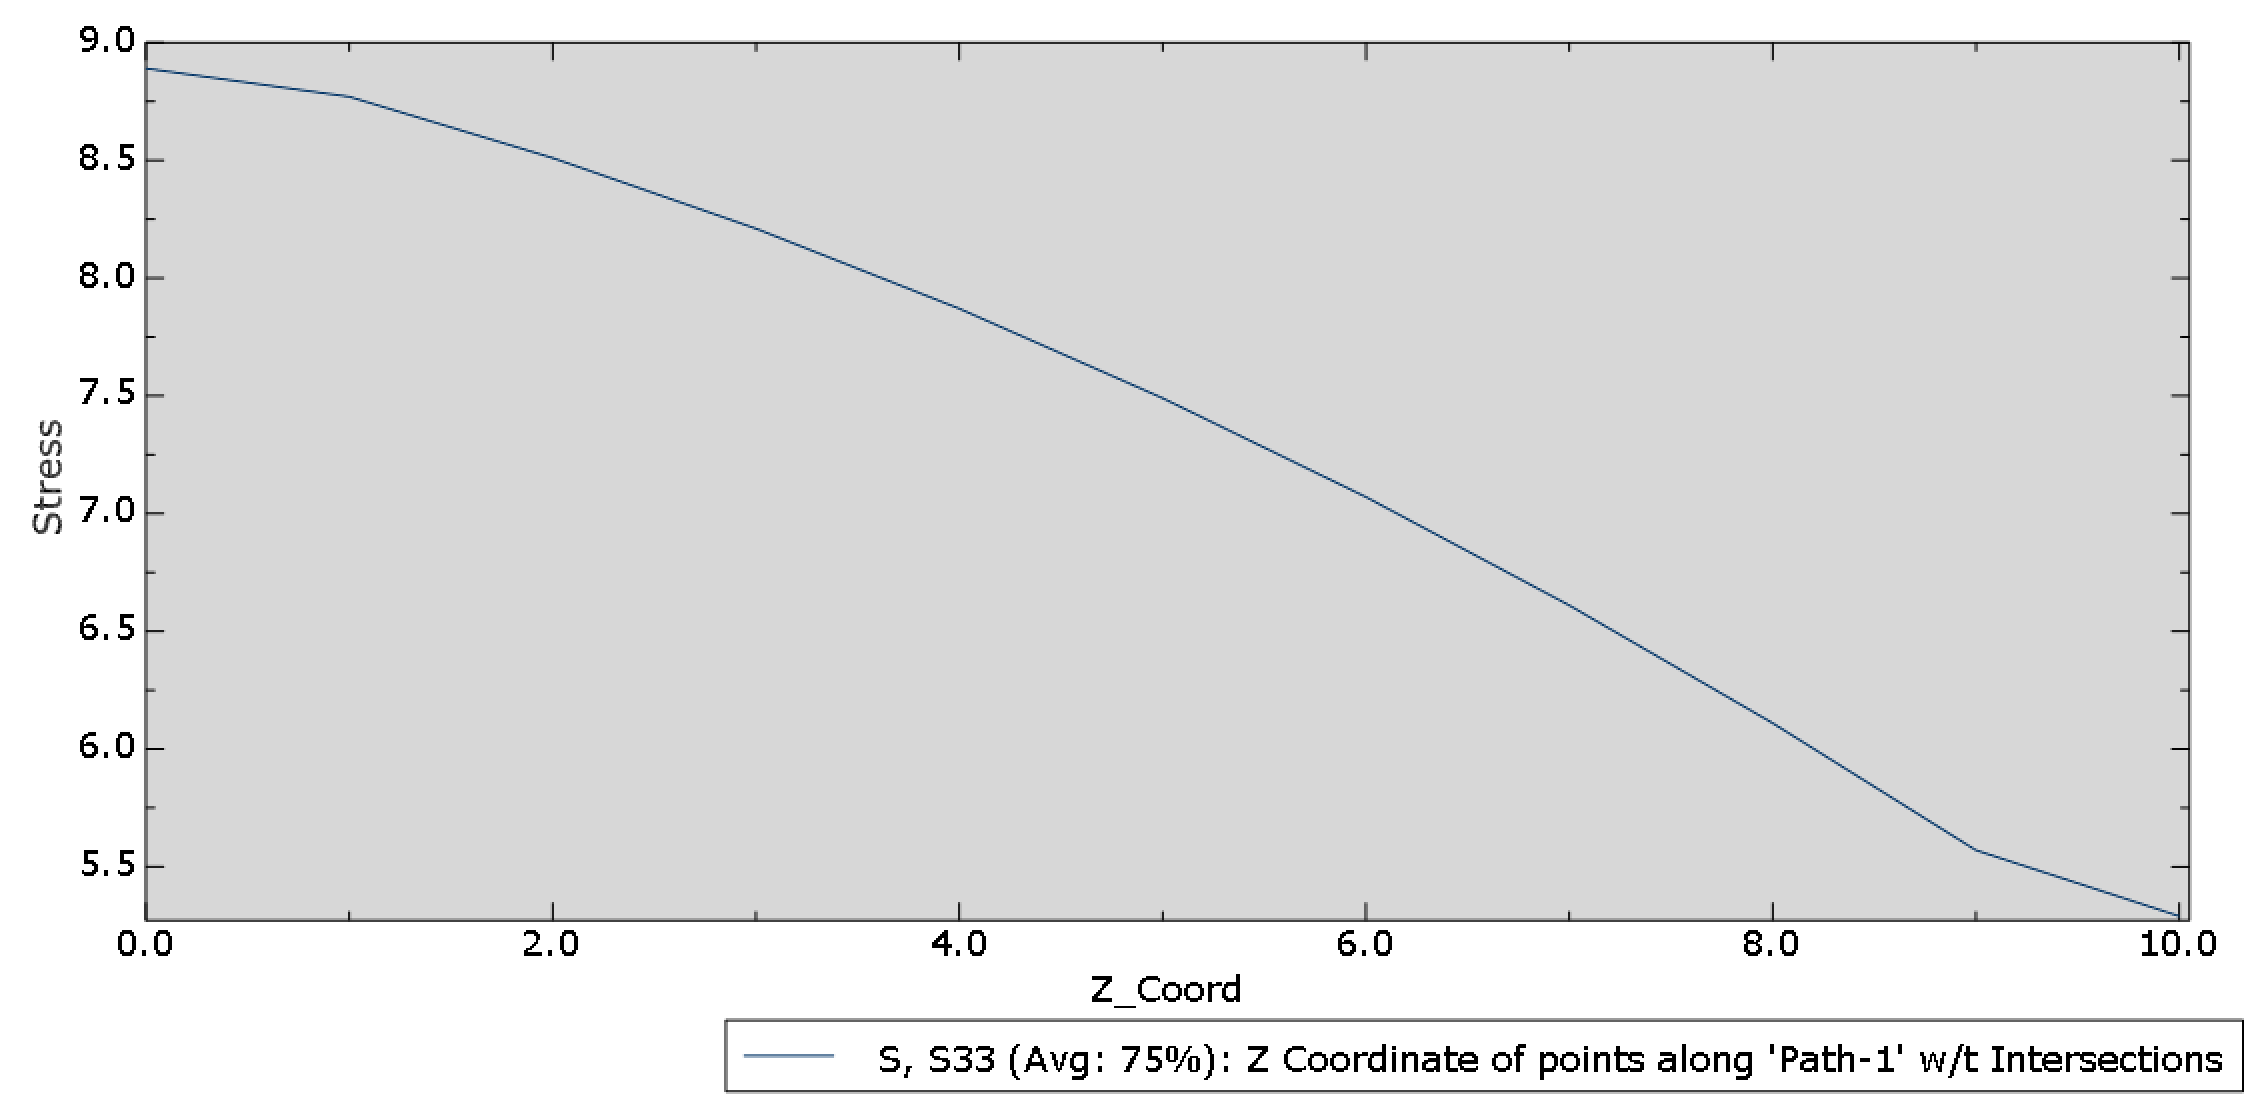
\includegraphics[scale=0.45]{capturas/S-data.png}
\caption{Tension $\sigma_z$ a lo largo del eje Z}
\label{fig:Data3}%
\end{figure}

Para ello lo realizamos de una manera distinta. Debemos escoger, en la pestaña ``Report/'' la opción \emph{Field Output}. Se nos abrira una ventana donde, en la pestaña \emph{Variable} deberemos seleccionar el Field S33 en los puntos de integración (figura \ref{fig:out1a}), mientras que en la pestaña Setup debemos denominar al  archivo \texttt{s33.csv} (figura \ref{fig:out1b}).

\begin{figure}
\centering
\captionsetup[subfigure]{justification=centering,singlelinecheck=false}
  \begin{subfigure}[b]{0.36\textwidth}
  \hspace{0mm}
    \imagebox{85mm}{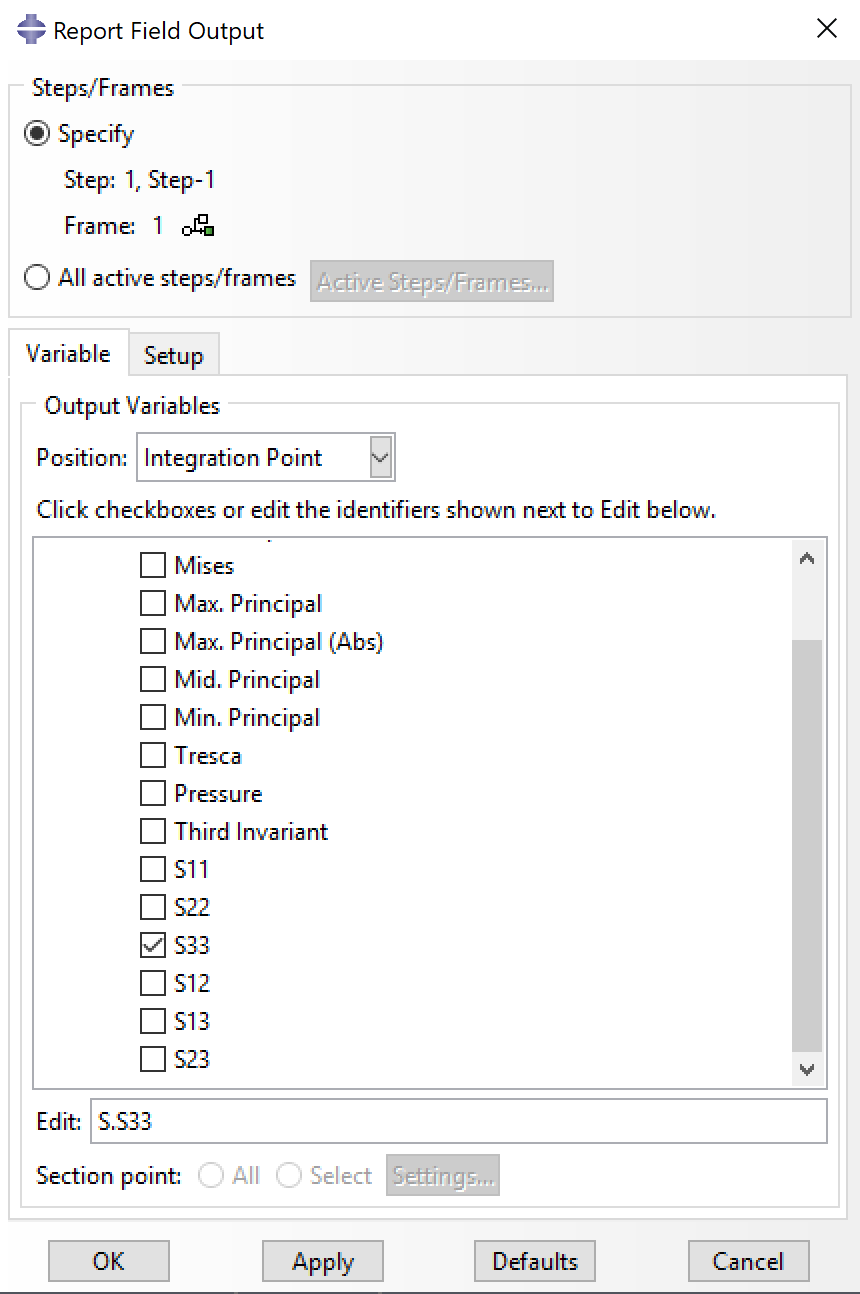
\includegraphics[scale=0.35]{capturas/out1.png}}
    \caption{Variable\label{fig:out1a}}
  \end{subfigure}
  \begin{subfigure}[b]{0.36\textwidth}
  \hspace{5mm}
    \imagebox{85mm}{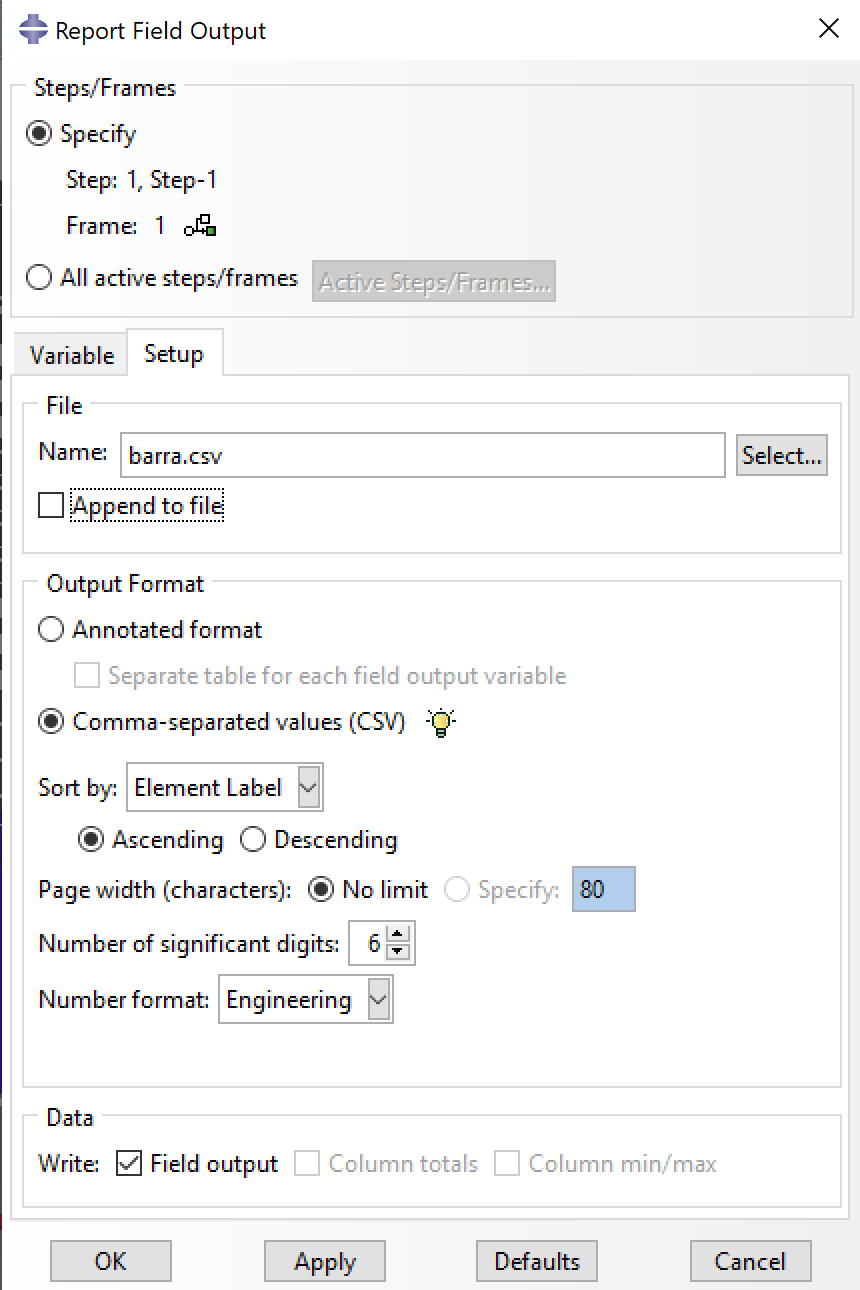
\includegraphics[scale=0.35]{capturas/out2.png}}
    \caption{Setup\label{fig:out1b}}
  \end{subfigure}
\caption{Field Output}
\label{fig:out1}
\end{figure}

\clearpage
\section{Ejemplo de programación elementos finitos en Python}
\label{sec:python}

A continuación se adjunta un \emph{Notebook} de \emph{Python} con el seguimiento de la creación de códigos y aplicación al caso de la barra 1D.

El archivo \texttt{*.ipynb} puede descargarse del siguiente repositorio, o bien abrir directamente en cualquier de los programas que a continuación se mencionarán:\\

\href{https://github.com/juanjosearribas/met_comp}{\textcolor{blue}{\texttt{Repositorio Git-Hub}}}\\

El \emph{Notebook} puede correrse el programa \texttt{Jupyter}, que pertenece a la suite \texttt{Anaconda}, suite en abierto para plataformas \emph{Windows, Mac y Linux}. Es necesario instalarse dicha suite y cargar el \emph{Notebook} bien abriendo el archivo \texttt{*.ipynb}, o bien desde el repositorio de Git-Hub antes mencionado.

Por otro lado, también nos encontramos soluciones que nos permiten correr el script sin necesidad de instalar ningún programa, son soluciones \emph{en la nube}. Entre otras, las más conocidas, son:

\begin{itemize}
\item  \href{https://colab.research.google.com}{\textcolor{blue}{\texttt{Colab de Google}}} Es necesario tener cuenta de Gmail.
\item  \href{http://mybinder.org/}{\textcolor{blue}{\texttt{MyBinder}}} Solo desde repositorio Git-Hub
\end{itemize}

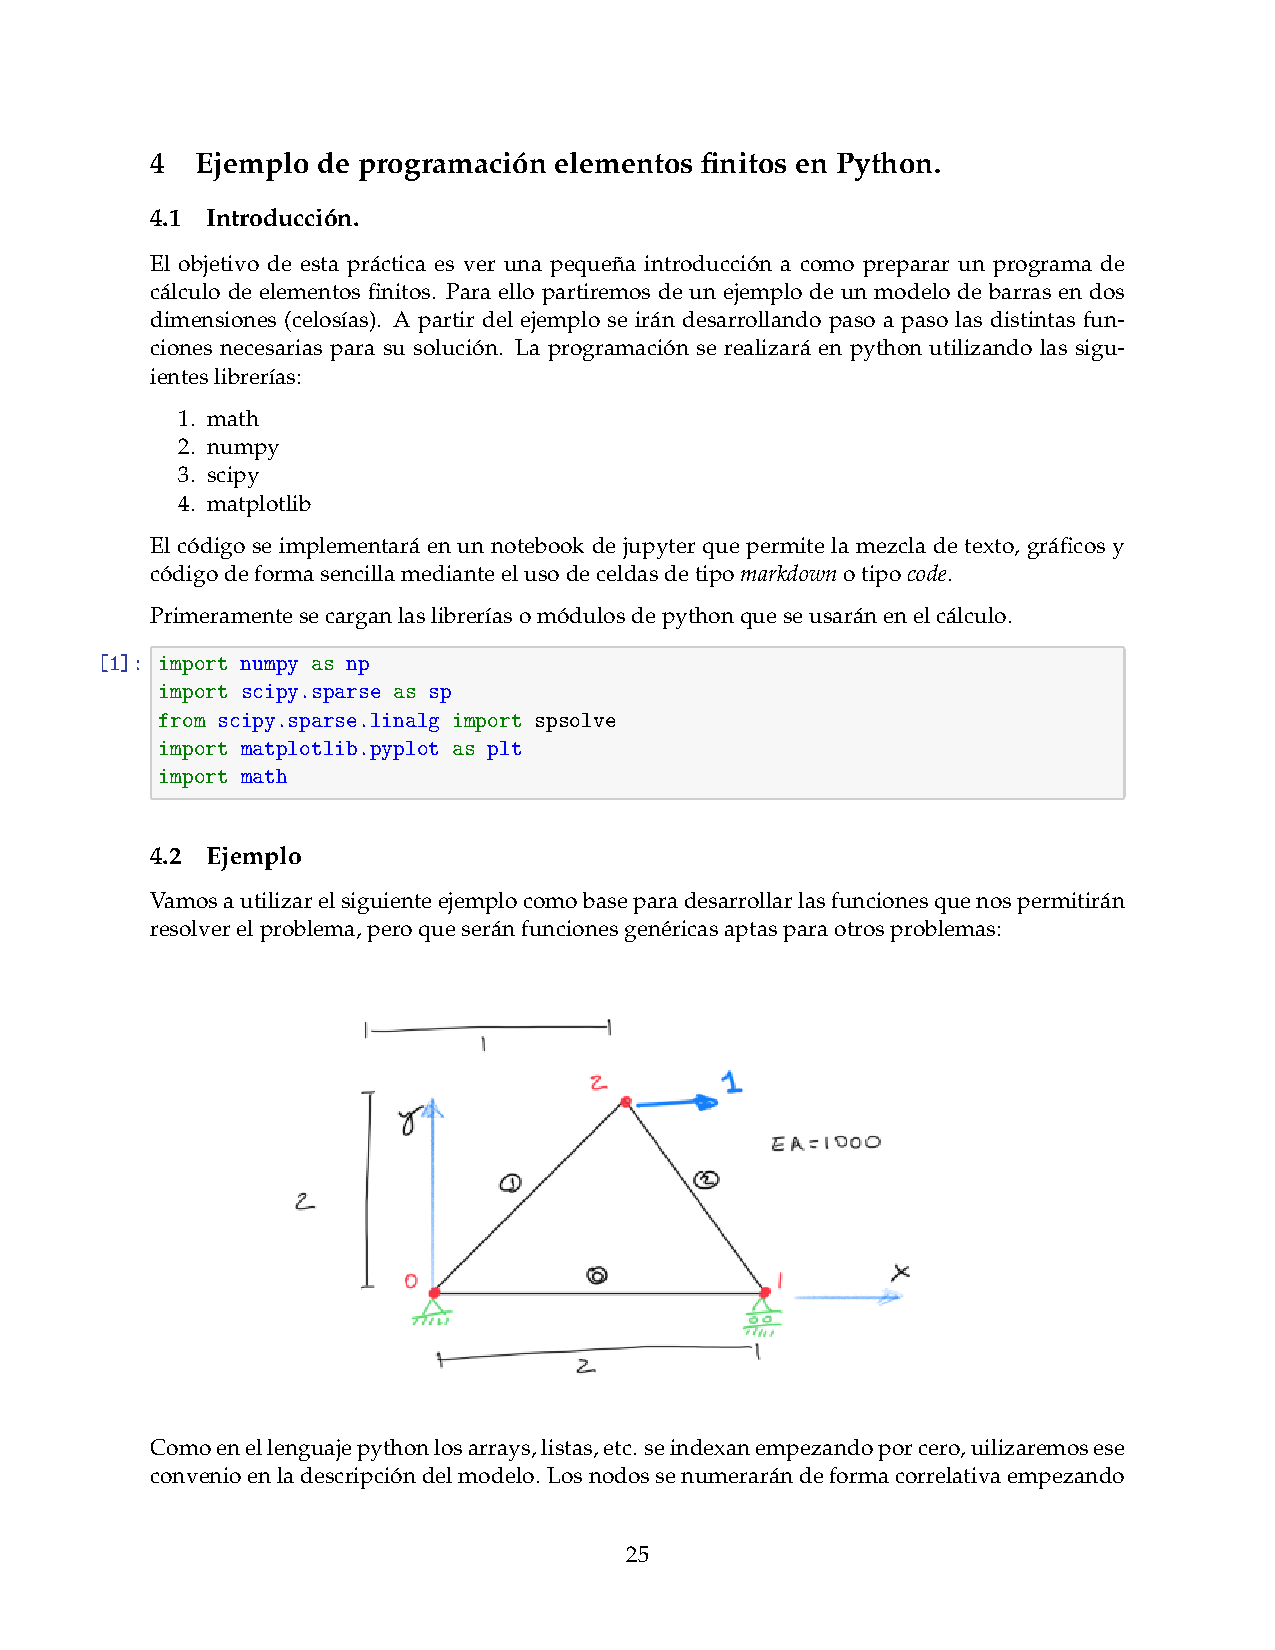
\includepdf[pages=-]{python_to_tex/el_fin2d_OK}


\clearpage
\appendix
\numberwithin{equation}{section}
\section{Simulación con MatLab / Octave}
\label{sec:matlab}

A continuación se expone la misma solución realizada en \texttt{MatLab}, para todo aquel que domine el lenguaje de programación de esta herramienta y quiera comprobar dicho problema también con este programa.

\subsection*{Código MatLab / Octave}
\label{sec:esq}

La organización del código en \texttt{Matlab} / \texttt{Octave} es libre, pero, puesto que es la primera aproximación que el alumno hace a un código de elementos finitos, el seguir los esquemas propuestos a continuación puede resultar muy interesante para tener unas pautas.

\begin{itemize}
\item Preproceso

A continuación se describe el preproceso, donde material, geometría, condiciones de contorno y mallado son definidas. Se debe también, según el tipo de problema y los grados de libertad que tenga el problema, definir el número de grados de libertad totales.


\begin{lstlisting}[ label=codigo1,caption=Esquema Matlab \emph{(a)}]
% Definición de parámetros particulares de cada alumno:
Nmat=1124                      % número de matrícula del alumno
m=floor(Nmat/1000)             % cifra de millares
c=floor((Nmat-m*1000)/100)     % cifra de centenas
d=floor((Nmat-m*1000-c*100)/10) % cifra de decenas
u=Nmat-m*1000-c*100-d*10       % cifra de unidades

% A: PREPROCESO
%----------------------------------------------------------------

% 1. Geometría
A=1;              % Area
L=10;             % Longitud de la barra

% 2. Material
E=1000;           % Módulo elástico

% 3. Condiciones de contorno en carga
P=5;                % dato de fuerza aplicada en x=L
q0=d/10;            % Fuerza volumetrica en x=0
qf=q0+u/10;         % Fuerza volumétrica en x=L

% 4. Malla
Nele=11-c;          % número de elementos
Nnod=Nele+1;        % número de nodos
q=linspace(q0,qf,Nnod);
h=L/Nele;			% tamano de cada elemento

% 5. Grados de Libertad del problema
% Dim = GDL totales = grados de libertad nodales x num. nodos
gdl=1;
Dim=Nnod*gdl;

\end{lstlisting}

\item Construcción de matrices elementales y globales

La primera parte del \textit{solver} trata de construir, a partir de las matrices elementales, y tras el ensamblado, las matrices globales de rigidez y carga. La matriz de rigidez elemental es igual para todos los elementos, al tratarse de elementos del mismo tamaño y propiedades constantes. En cambio, la de fuerza volumétrica, en este caso varía, por ser una carga que varía a lo largo de la barra. Finalmente, en el último nodo, se ha de aplicar la carga externa de 5 N.

\begin{lstlisting}[ label=codigo2,caption=Esquema Matlab \emph{(b)}]
% B: CONSTRUCCIÓN de MATRICES y VECTORES globales
%----------------------------------------------------------------
% 0. Inicialización
K=zeros(Dim);
F=zeros(Dim,1);
Fext=zeros(Dim,1); 

% 1. Matriz de rigidez elemental (común a todos los elementos)
k=(E*A/h)*[1,-1;-1,1];  

% 2. Ensamblaje de la matriz global
for i=1:Nele
    K(i:i+1,i:i+1)=K(i:i+1,i:i+1)+k;        % ensambla rigidez
end

% 3. Ensamblaje del vector de fuerzas volumetricas global
for i=1:Nele
    % vector elemental de cargas distribuidas
    fvol=(h/6)*[2*q(i)+q(i+1);q(i)+2*q(i+1)];
    % ensambla cargas
    F(i:i+1)=F(i:i+1)+fvol;                    
end

% 4. Suma del vector de fuerzas externas
Fext(Nnod)=Fext(Nnod)+P;
F=F+Fext;           % suma cargas en contorno y cargas distribuidas
\end{lstlisting}

\item Aplicación de condiciones de contorno y resolución

Para el núcleo central del \textit{solver} es necesario aplicar las condiciones de contorno, reduciendo el sistema matricial y, finalmente, invirtiendo esta matriz reducida. Se comprueba el equilibrio a posteriori.

\begin{lstlisting}[ label=codigo3,caption=Esquema Matlab \emph{(c)}]
% C: APLICACIÓN de las CONDICIONES de CONTORNO y RESOLUCIÓN
%----------------------------------------------------------------

% 1. Reducción de la matriz de rigidez
Kg=K(2:Nnod,2:Nnod);

% 2. Reducción del vector de fuerzas
Fg=F(2:Nnod);

% 3. Resuelve sistema reducido para desplazamientos
ug=Kg\Fg;

% 4. Desplazamientos y reacciones. Equilibrio: Sum fuerzas = 0
un=[0;ug];
fint=K*un;
r_0=fint(1)-F(1);
Eq=sum(fint);
if abs(Eq)>1e-10
    Disp('Equilibrio no alcanzado');
end
\end{lstlisting}

\item Postproceso

Dentro del postproceso nos interesa calcular las deformaciones y a través de ellas las tensiones a nivel elemental. Una vez calculada la solución analítica tanto de tensiones como de desplazamientos (ecuaciones \eqref{eq:analitica}), podemos  realizar una comparativa con nuestros resultados, a nivel nodal de los desplazamientos y a nivel elemental de las tensiones.

\begin{lstlisting}[ label=codigo4,caption=Esquema Matlab \emph{(d)}]

% D: POSTPROCESO
%----------------------------------------------------------------

% 1. Deformaciones y Tensiones
epsilon=zeros(Nele,1);
for i=1:Nele
    epsilon(i)=(un(i+1)-un(i))/h;
end
sigma=E*epsilon;

% 2. Solución analítica
dx=20;
xc=linspace(0,L,dx);
dq=qf-q0;
r=dq/L;
uc=1/(E*A)*((P+q0*L+1/2*r*L^2)*xc-(1/2*q0*xc.^2+1/6*r*xc.^3));
sigmac=1/A*(P+q0*(L-xc)+1/2*r*(L^2-xc.^2));

% 3. Gráfico

% 3.1. Dibuja la solucion del desplazamiento en x
figure 
xn=linspace(0,L,Nele+1);
plot(xn,un,'-+',xc,uc,'-','LineWidth',2,'MarkerSize',10);
% hold
title(['Ejercicio de fibra elástica 1D MEF, Nmat=' num2str(Nmat)]);
legend({'Solución MEF','Solución analitica'},'Location','Northwest');
xlabel('Coordenada x (mm)');
ylabel('Desplazamiento u (mm)');

% 3.2. Dibuja la solucion de la tensión en x
figure
xe=linspace(h/2,Nele*h-h/2,Nele); 
plot(xe,sigma,'o',xc,sigmac,'-','LineWidth',2,'MarkerSize',10);
hold;
xs=linspace(0,L,Nele+1);
stairs(xs,[sigma;sigma(Nele)],'LineWidth',2);
title(['Ejercicio de fibra elástica 1D MEF, Nmat=' num2str(Nmat)]);
legend({'Solución MEF','Solución analitica'},'Location','Northeast');
xlabel('Coordenada x (mm)');
ylabel('Tensión \sigma (N/mm^2)');

pause;

\end{lstlisting}

A continuación, en la figura \ref{fig:solmatlab}, podemos ver la solución obtenida con el código que hemos desarrollado en \texttt{MatLab} / \texttt{Octave} y la solución analítica a partir de las ecuaciones \eqref{eq:analitica}. Como vemos, la solución de los desplazamientos ha sido obtenida en los nodos, por lo que a la localización de cada nodo se corresponderá un valor del desplazamiento. En cambio, las tensiones son obtenidas en los puntos de integración de los elementos, en este caso un punto por elemento en el medio del mismo. Por ello debemos dibujar el valor de las tensiones en la localización de los puntos de integración. Además hemos añadido la función \emph{stairs} para resaltar que el valor de las tensiones es constante en cada elemento.

\begin{figure}[h!tp]
\centering
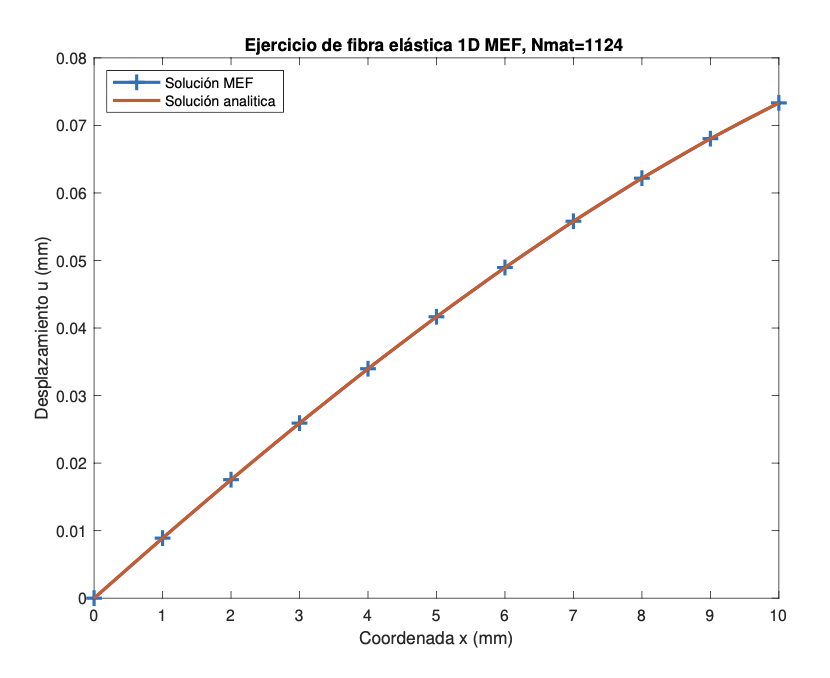
\includegraphics[width=0.5\textwidth]{figuras/u-matlab.png}%
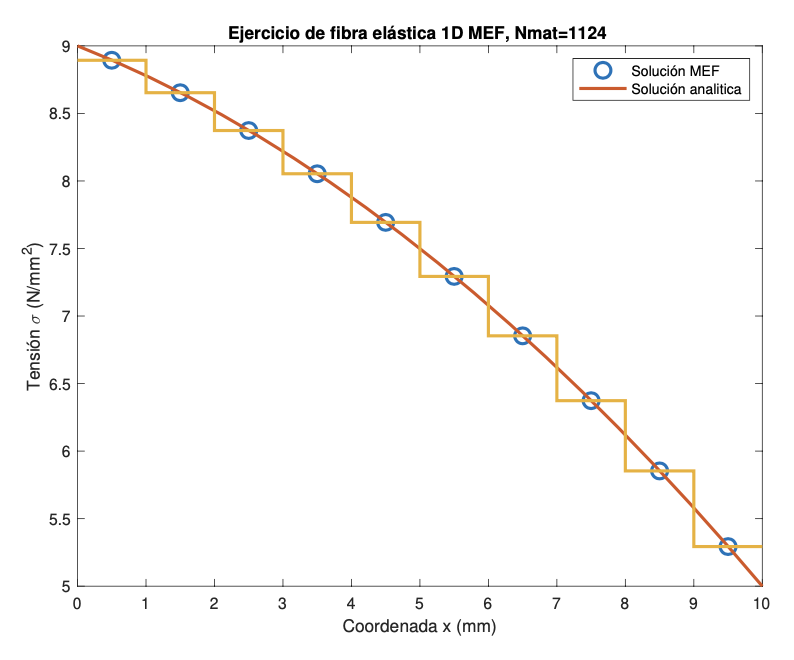
\includegraphics[width=0.5\textwidth]{figuras/s-matlab.png}
%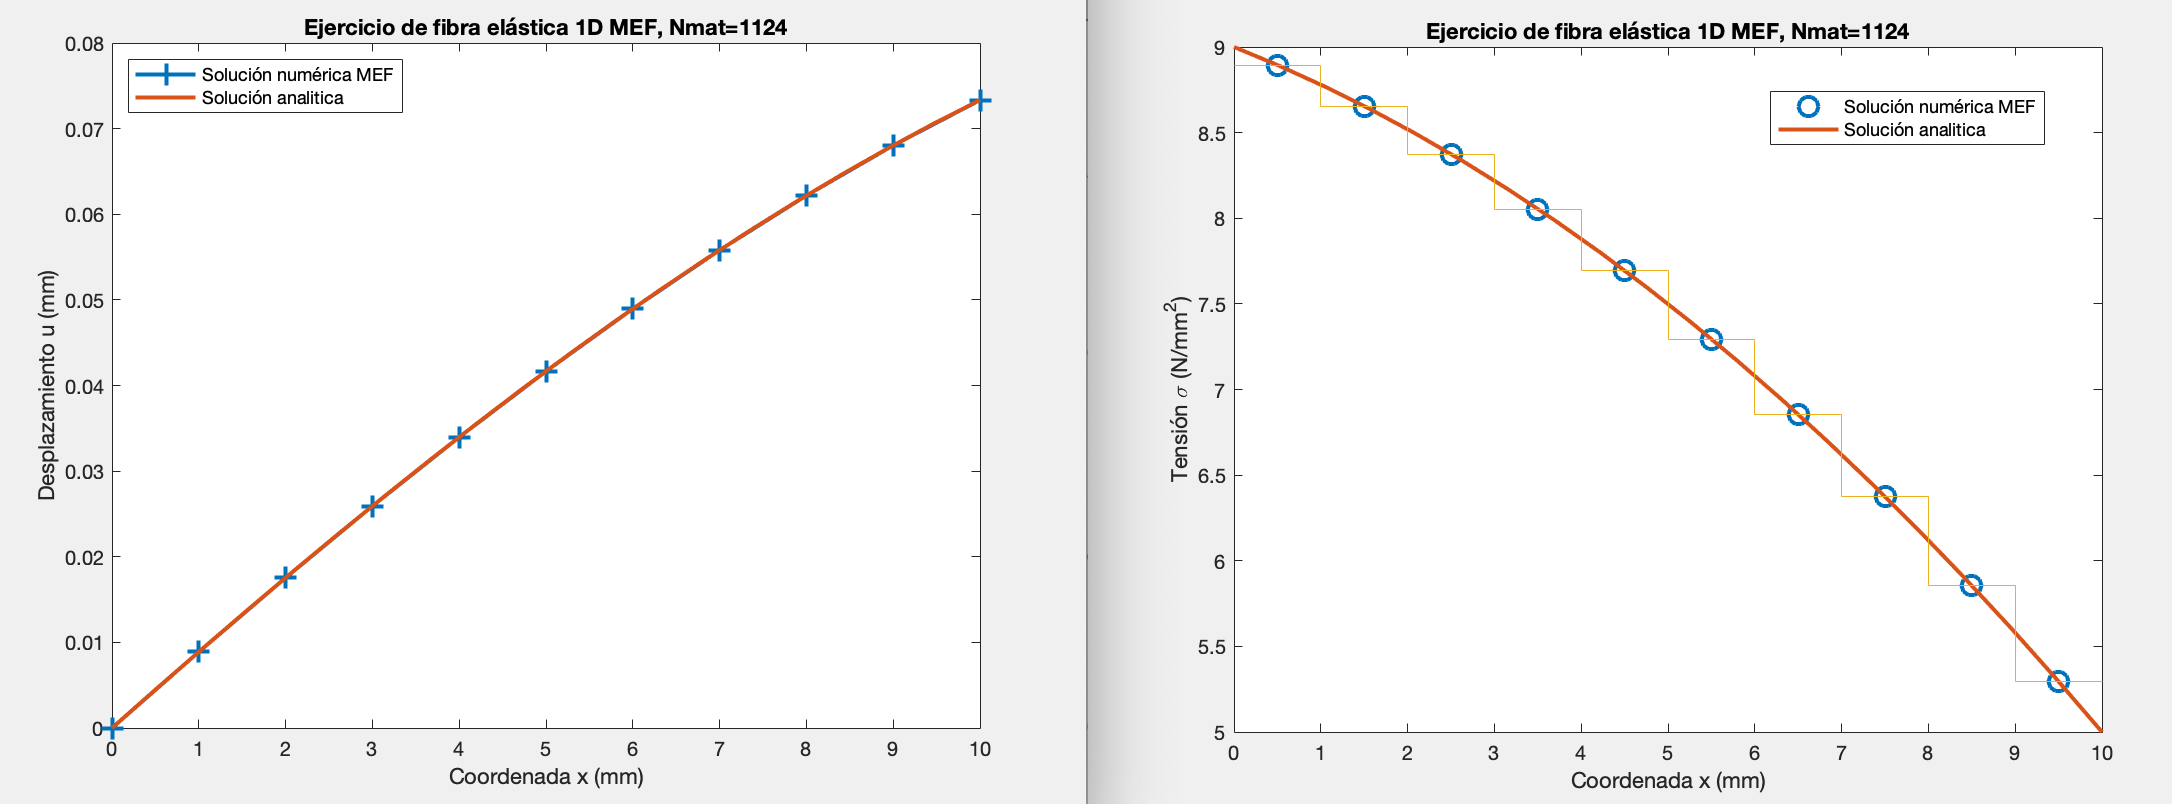
\includegraphics[scale=0.45]{capturas/sol_matlab.png}
\caption{Comparación entre la solución obtenida con MatLab y la solución analítica.}
\label{fig:solmatlab}
\end{figure}

\item Comparativa con solución analítica en \texttt{MatLab} / \texttt{Octave}

En primer lugar debemos dejar preparado el código de \texttt{MatLab} / \texttt{Octave} para introducir los datos procedentes de \emph{Abaqus}. A continuación se presenta el código, similar al de postproceso empleado anteriormente.
\begin{lstlisting}[ label=codigo5,caption=Esquema Matlab-Abaqus]
% E: ABAQUS
%----------------------------------------------------------------

xn_ab=[

    ]; 

un_ab=[

    ];

xe_ab=[                      

    ];

sigma_ab=[

    ];

% % 1. Dibuja la solucion del desplazamiento en x
figure 
plot(xn_ab,un_ab,'-+',xc,uc,'-','LineWidth',2,'MarkerSize',10)
%hold
title(['Ejercicio de fibra elástica 1D MEF, Nmat=' num2str(Nmat)])
legend({'Solución MEF Abaqus','Solución analitica'},'Location','Northwest')
xlabel('Coordenada x (mm)')
ylabel('Desplazamiento u (mm)')

% 2. Dibuja la solucion de la tensión en x
figure
plot(xe_ab,sigma_ab,'o',xc,sigmac,'-','LineWidth',2,'MarkerSize',10)
hold
xs=linspace(L,0,Nele+1);
stairs(xs,[sigma_ab;sigma_ab(Nele)],'LineWidth',2)
title(['Ejercicio de fibra elástica 1D MEF, Nmat=' num2str(Nmat)])
legend({'Solución MEF Abaqus','Solución analitica'},'Location','Northeast')
xlabel('Coordenada x (mm)')
ylabel('Tensión \sigma (N/mm^2)')
\end{lstlisting}

Como vemos, dejamos huecos para los vectores que provengan de los resultados de  \emph{Abaqus}. Los vectores los rellenamos con los datos que extraigamos de Abaqus. El resultado de la comparativa se ve en la figura \ref{fig:out3}. 
Se puede comprobar que el resultado es idéntico al obtenido con el programa 1D en Matlab, figura~\ref{fig:solmatlab} y el realizado en Python y como anteriormente también coinciden de forma exacta los valores discretos en los nodos y en el centro de los elementos con la solución analítica.

\begin{figure}[h!tp]
\centering
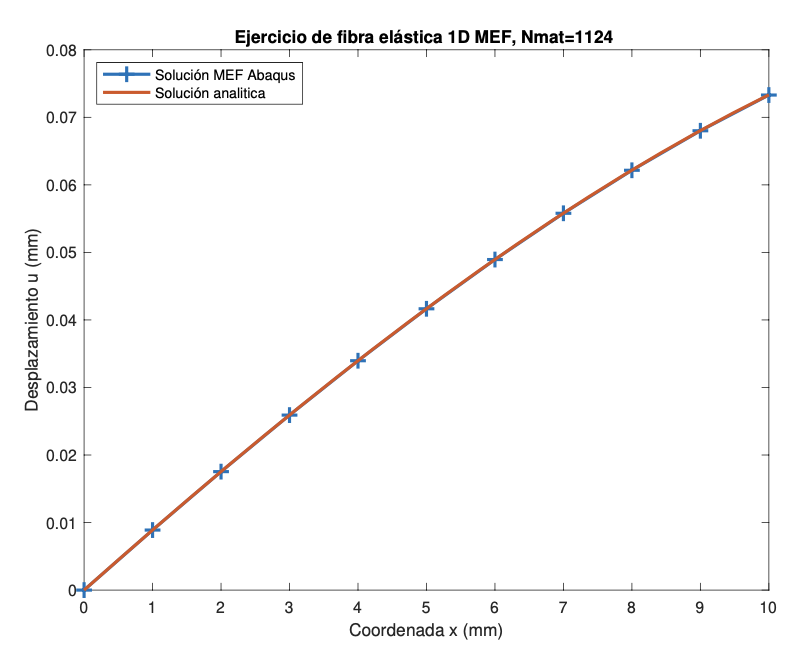
\includegraphics[width=0.5\textwidth]{figuras/u-abaqus.png}%
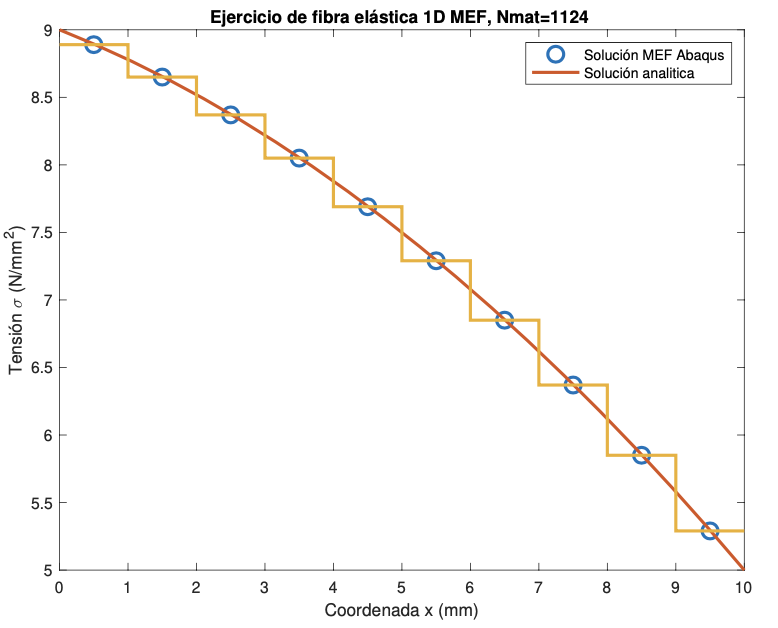
\includegraphics[width=0.5\textwidth]{figuras/s-abaqus.png}
%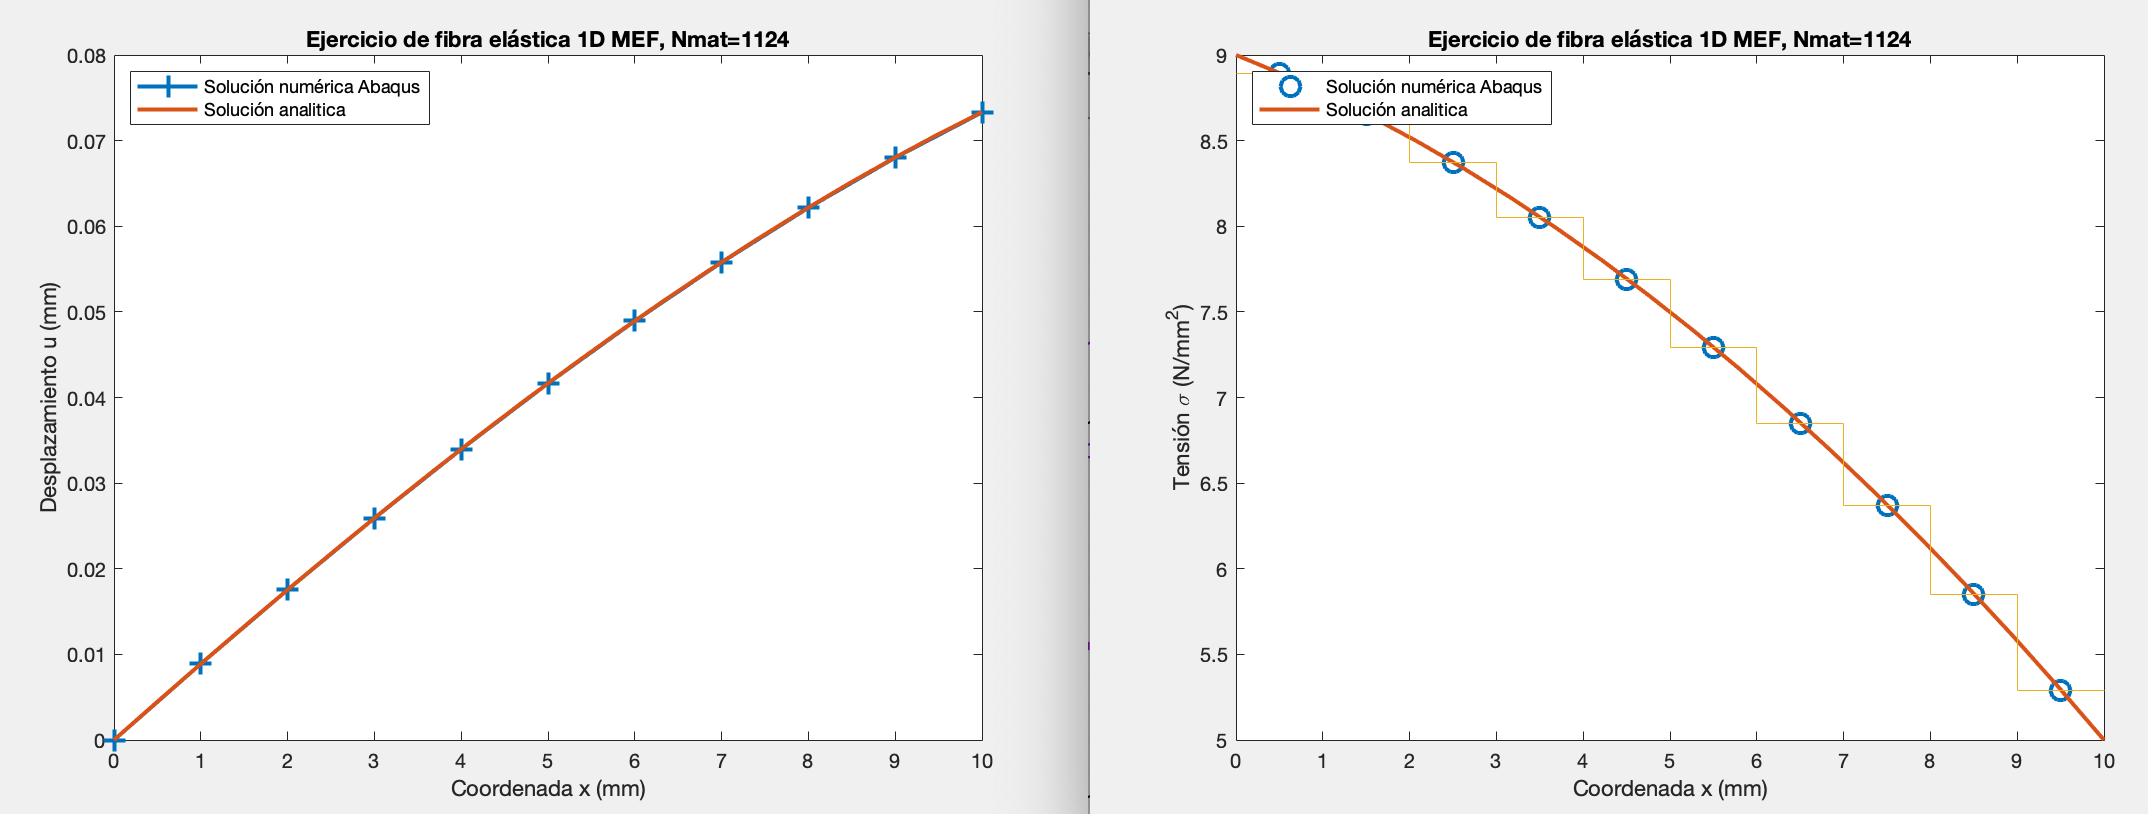
\includegraphics[scale=0.45]{capturas/out3.png}
\caption{Comparación entre la solución obtenida con \emph{Abaqus} y la solución analítica.}
\label{fig:out3}%
\end{figure}

\end{itemize}
%\begin{thebibliography}{10}
%\end{thebibliography}

\end{document}
